\documentclass[12pt,a4paper]{article}

% ================== PACKAGES ==================
\usepackage[margin=2.54cm]{geometry}
\usepackage[utf8]{inputenc}
\usepackage[T5]{fontenc}
\usepackage[vietnamese]{babel}
\usepackage{lmodern}
\usepackage{setspace}
\usepackage{booktabs}
\usepackage{array}
\usepackage{graphicx}
\usepackage{xcolor}
\usepackage{hyperref}
\usepackage{listings}
\usepackage{amsmath}
\usepackage{amssymb}
\usepackage{enumitem}
\usepackage{fancyhdr}
\usepackage{titlesec}
\usepackage{xurl}
\usepackage{float}
\usepackage{tocloft}
\usepackage{csquotes}
\usepackage{tikz}
\usetikzlibrary{arrows.meta, positioning, calc, matrix, decorations.pathreplacing}

% ================== REFERENCES ==================
\usepackage[
    backend=biber,
    style=ieee,
    sorting=none
]{biblatex}

\addbibresource{references.bib}

% ================== FONT & SPACING ==================
\onehalfspacing

% ================== PARAGRAPH FORMAT ==================
\setlength{\parindent}{1.25cm}
\setlength{\parskip}{0pt}

% ================== HYPERREF SETUP ==================
\hypersetup{
    colorlinks=true,
    linkcolor=blue,
    citecolor=blue,
    urlcolor=cyan,
    pdftitle={Ranking},
    pdfauthor={Group 07}
}

% ================== HEADER & FOOTER ==================
\pagestyle{fancy}
\fancyhf{}
\lhead{Một số chủ đề trong Học máy}
\rhead{Ranking}
\rfoot{Trang \thepage}

% ================== TITLE FORMAT ==================
\titleformat{\section}
    {\Large\bfseries}
    {\thesection}
    {1em}
    {}

\titleformat{\subsection}
    {\large\bfseries}
    {\thesubsection}
    {1em}
    {}

\titleformat{\subsubsection}
    {\normalsize\bfseries}
    {\thesubsubsection}
    {1em}
    {}

% ================== LISTING SETUP ==================
\lstset{
    basicstyle=\ttfamily\small,
    breaklines=true,
    frame=single,
    numbers=left,
    numberstyle=\tiny,
    keywordstyle=\color{blue},
    commentstyle=\color{gray},
    stringstyle=\color{red}
}

% ================== CUSTOM COMMANDS ==================
\newcommand{\abbr}[2]{#1 & #2 \\}

% ================== VIETNAMESE NAMES ==================
\renewcommand{\contentsname}{Mục lục}
\renewcommand{\listfigurename}{Danh mục hình vẽ}
\renewcommand{\listtablename}{Danh mục bảng}
\renewcommand{\figurename}{Hình}
\renewcommand{\tablename}{Bảng}

% ================== DOCUMENT ==================
\begin{document}

% ================== TITLE PAGE ==================
\begin{titlepage}
\begin{center}

{\large
ĐẠI HỌC QUỐC GIA THÀNH PHỐ HỒ CHÍ MINH\\
TRƯỜNG ĐẠI HỌC KHOA HỌC TỰ NHIÊN\\
KHOA CÔNG NGHỆ THÔNG TIN
}\\[3.0cm]


\includegraphics[width=4cm]{logo-khtn.png}\\[1.5cm]

{\color{blue}\LARGE \textbf{ĐỒ ÁN 2}}\\[0.5cm]
{\LARGE \textbf{RANKING TRONG HỌC MÁY}}\\[2.5cm]

\begin{tabular}{ll}
\textbf{Mã số sinh viên} & \textbf{Họ và tên} \\[0.2cm]
23120245 & NGUYỄN QUANG DUY \\
23120258 & LƯU TRỌNG HIẾU \\
23120260 & VĂN ĐÌNH HIẾU \\
\end{tabular}

\vfill

\begin{tabular}{ll}
\textbf{Giảng viên hướng dẫn} & TS Bùi Tiến Lên \\
                              & Th.S Lê Nhựt Nam \\
\end{tabular}

\vfill

\begin{tabular}{ll}
\textbf{Môn học} & Nhập môn Học máy \\
\end{tabular}

\vspace{0.3cm}

\textbf{Thành phố Hồ Chí Minh -- 2026}

\end{center}
\end{titlepage}

% ================== FRONT MATTER ==================
\pagenumbering{roman}

% ================== ABSTRACT ==================
\section*{Tóm tắt}
\addcontentsline{toc}{section}{Tóm tắt}

Báo cáo này trình bày chủ đề Ranking trong học máy dựa trên nội dung chương 	\textit{Ranking} của sách 	\textit{Foundations of Machine Learning}. Nội dung tập trung vào các khái niệm nền tảng như hàm điểm, quan hệ ưu tiên, ranking loss, margin trong ranking, score-based ranking, SVM-ranking, RankBoost, bipartite ranking, ROC/AUC và preference-based ranking. Bên cạnh phần lý thuyết, báo cáo cũng thảo luận các tiêu chí đánh giá ranking như pairwise accuracy, ranking loss, Kendall tau distance, AUC, MAP, MRR và NDCG.

Phần thực nghiệm lựa chọn pairwise ranking làm trọng tâm. Nhóm cài đặt từ đầu một mô hình scoring tuyến tính bằng NumPy, huấn luyện bằng pairwise hinge loss trên dữ liệu tổng hợp, và đánh giá kết quả thông qua pairwise accuracy, ranking loss, Kendall tau distance và top-\(k\) overlap. Thực nghiệm nhằm minh hoạ mối liên hệ giữa lý thuyết ranking theo từng cặp và quá trình tối ưu mô hình trong thực hành.

\newpage

% ================== TABLE OF CONTENTS ==================
\tableofcontents
\newpage

% ================== ABBREVIATIONS ==================
\section*{Danh mục từ viết tắt}
\addcontentsline{toc}{section}{Danh mục từ viết tắt}

\begin{center}
\begin{tabular}{ll}
\toprule
\textbf{Từ viết tắt} & \textbf{Ý nghĩa} \\
\midrule
LTR & Learning to Rank \\
ML & Machine Learning \\
SVM & Support Vector Machine \\
ROC & Receiver Operating Characteristic \\
AUC & Area Under the ROC Curve \\
TPR & True Positive Rate \\
FPR & False Positive Rate \\
NDCG & Normalized Discounted Cumulative Gain \\
DCG & Discounted Cumulative Gain \\
IDCG & Ideal Discounted Cumulative Gain \\
MAP & Mean Average Precision \\
AP & Average Precision \\
MRR & Mean Reciprocal Rank \\
RR & Reciprocal Rank \\
\bottomrule
\end{tabular}
\end{center}

\newpage

% ================== LIST OF FIGURES ==================
\listoffigures
\addcontentsline{toc}{section}{Danh mục hình vẽ}
\newpage

% ================== LIST OF TABLES ==================
\listoftables
\addcontentsline{toc}{section}{Danh mục bảng}
\newpage

% ================== MAIN MATTER ==================
\pagenumbering{arabic}
\setcounter{figure}{0}
\setcounter{table}{0}

\section{Giới thiệu}

Trong nhiều bài toán học máy hiện đại, mục tiêu của mô hình không chỉ là dự đoán một nhãn rời rạc hoặc một giá trị số, mà còn là sắp xếp một tập các đối tượng theo một thứ tự mong muốn. Bài toán này được gọi là \textit{ranking} hoặc \textit{learning to rank}. Ranking xuất hiện tự nhiên trong nhiều ứng dụng thực tế như xếp hạng kết quả tìm kiếm, gợi ý sản phẩm, sắp xếp tài liệu theo mức độ liên quan, xếp hạng ứng viên, hoặc đánh giá mức độ ưu tiên của các hành động trong một hệ thống ra quyết định.

Khác với bài toán phân loại, trong đó mỗi mẫu thường được gán vào một lớp cụ thể, ranking quan tâm đến quan hệ thứ tự giữa các đối tượng. Ví dụ, trong hệ thống tìm kiếm, điều quan trọng không chỉ là xác định một tài liệu có liên quan hay không, mà còn là tài liệu nào nên được đặt ở vị trí cao hơn trong danh sách kết quả. Do đó, ranking thường được mô hình hoá thông qua các hàm điểm, quan hệ ưu tiên giữa các cặp đối tượng, hoặc các độ đo đánh giá chất lượng của toàn bộ danh sách xếp hạng.

Trong báo cáo này, nhóm tập trung tìm hiểu chủ đề Ranking dựa trên nội dung trong sách \textit{Foundations of Machine Learning}. Mục tiêu chính là trình bày lại các khái niệm nền tảng của ranking bằng tiếng Việt, giải thích ý nghĩa trực giác của các định nghĩa và công thức, đồng thời minh hoạ lý thuyết bằng thực nghiệm lập trình. Báo cáo không chỉ xem ranking như một bài toán ứng dụng, mà còn phân tích các cách tiếp cận lý thuyết phổ biến như \textit{pointwise ranking}, \textit{pairwise ranking} và \textit{listwise ranking}.

Trong ba hướng tiếp cận trên, phần thực nghiệm của báo cáo chọn \textit{pairwise ranking} làm trọng tâm. Lý do là pairwise ranking có mối liên hệ trực tiếp với quan hệ ưu tiên giữa hai đối tượng, ranking loss, và reduction từ ranking sang classification. Bên cạnh đó, hướng tiếp cận này có thể được cài đặt từ đầu bằng các phép toán tuyến tính cơ bản, phù hợp với mục tiêu minh hoạ lý thuyết bằng Python và NumPy. Cụ thể, nhóm xây dựng một mô hình scoring tuyến tính, sinh dữ liệu tổng hợp, tạo các cặp preference, huấn luyện mô hình bằng pairwise hinge loss, và đánh giá kết quả thông qua các độ đo như pairwise accuracy, ranking loss và Kendall tau distance.

Báo cáo được tổ chức như sau. Phần đầu trình bày các khái niệm chuẩn bị cần thiết cho bài toán ranking, bao gồm scoring function, preference relation và ranking loss. Tiếp theo, báo cáo giới thiệu ba hướng tiếp cận chính trong learning to rank: pointwise, pairwise và listwise. Sau đó, phần lý thuyết chính tập trung vào pairwise ranking, cách xây dựng dữ liệu dạng cặp, hàm mất mát pairwise hinge loss và mối liên hệ với bài toán classification. Phần thực nghiệm mô tả quá trình cài đặt mô hình ranking tuyến tính từ đầu, thiết kế dữ liệu tổng hợp, các độ đo đánh giá và phân tích kết quả. Cuối cùng, báo cáo thảo luận một số hướng nghiên cứu hiện đại liên quan đến ranking, đồng thời tổng kết những kết quả đạt được và các hạn chế còn tồn tại.
\section{Kiến thức chuẩn bị}
\label{sec:kien-thuc-chuan-bi}

Chương Ranking nghiên cứu các bài toán học máy trong đó đầu ra của mô hình là một thứ tự xếp hạng giữa các đối tượng. Khác với phân loại, ranking không chỉ hỏi một mẫu thuộc lớp nào, mà quan tâm đối tượng nào nên đứng trước đối tượng nào. Bài toán này xuất hiện trong công cụ tìm kiếm, hệ thống gợi ý, truy xuất thông tin, xếp hạng sản phẩm, xếp hạng phim và phát hiện gian lận.

\subsection{Bài toán xếp hạng}

Gọi \(\mathcal{X}\) là không gian đầu vào. Với một tập hữu hạn gồm \(n\) đối tượng:
\[
    X=\{x_1,x_2,\ldots,x_n\}\subseteq \mathcal{X},
\]
mục tiêu của ranking là tìm một thứ tự sao cho các đối tượng quan trọng hơn hoặc liên quan hơn được đặt ở vị trí cao hơn. Nếu \(x_i\) nên được xếp trước \(x_j\), ta viết:
\[
    x_i \succ x_j.
\]

Một ranking đầy đủ có thể được biểu diễn bởi một hoán vị \(\pi\) của tập chỉ số \(\{1,2,\ldots,n\}\):
\[
    x_{\pi(1)} \succ x_{\pi(2)} \succ \cdots \succ x_{\pi(n)}.
\]

\subsection{Hàm điểm và ranking dựa trên điểm số}

Một cách phổ biến để tạo ranking là học một hàm điểm:
\[
    h:\mathcal{X}\rightarrow\mathbb{R}.
\]
Hàm \(h\) gán cho mỗi đối tượng một điểm số thực. Nếu \(h(x_i)>h(x_j)\), mô hình xếp \(x_i\) cao hơn \(x_j\). Do đó, ranking được tạo bằng cách sắp xếp các đối tượng theo điểm số giảm dần:
\[
    h(x_{\pi(1)})\geq h(x_{\pi(2)})\geq \cdots \geq h(x_{\pi(n)}).
\]

Trong nhiều mô hình, mỗi đối tượng được biểu diễn bởi vector đặc trưng \(x_i\in\mathbb{R}^d\). Một lớp hàm điểm đơn giản và quan trọng là hàm tuyến tính:
\[
    h_w(x)=w^\top x,
\]
trong đó \(w\in\mathbb{R}^d\) là vector tham số cần học.

\begin{figure}[H]
    \centering
    \begin{tikzpicture}[>=Stealth]
        \draw[->, thick] (0,0) -- (10.5,0) node[right] {điểm \(h(x)\)};
        \foreach \x/\label/\score in {1.2/\(x_4\)/0.4, 3.0/\(x_2\)/1.1, 5.2/\(x_5\)/1.8, 7.4/\(x_1\)/2.6, 9.0/\(x_3\)/3.1} {
            \draw[fill=gray!30] (\x,0) circle (3pt);
            \node[above] at (\x,0.05) {\label};
            \node[below] at (\x,-0.05) {\(\score\)};
        }
        \draw[->, thick, dashed] (9.2,0.8) -- (1.0,0.8);
        \node[above] at (5.1,0.8) {sắp xếp giảm dần theo điểm số};
    \end{tikzpicture}
    \caption{Score-based ranking tạo thứ tự bằng cách sắp xếp các đối tượng theo điểm số \(h(x)\).}
    \label{fig:section2-score-axis-ranking-short}
\end{figure}

\subsection{Quan hệ ưu tiên theo từng cặp}

Dữ liệu huấn luyện trong ranking thường được cho dưới dạng các cặp đối tượng:
\[
    (x_i,x'_i,y_i)\in
    \mathcal{X}\times\mathcal{X}\times\{-1,0,+1\}.
\]
Nhãn \(y_i\) biểu diễn quan hệ ưu tiên giữa \(x_i\) và \(x'_i\):
\[
    y_i =
    \begin{cases}
        +1, & \text{nếu } x'_i \text{ được ưu tiên hơn } x_i,\\
        -1, & \text{nếu } x_i \text{ được ưu tiên hơn } x'_i,\\
        0,  & \text{nếu hai đối tượng ngang nhau hoặc không có thông tin.}
    \end{cases}
\]

Với quy ước này, một cặp được xếp đúng khi:
\begin{equation}
    y_i\big(h(x'_i)-h(x_i)\big)>0.
    \label{eq:correct-pairwise-ranking}
\end{equation}
Biểu thức trên kiểm tra xem dấu của hiệu điểm giữa hai đối tượng có phù hợp với nhãn ưu tiên hay không.

\subsection{Lỗi xếp hạng theo từng cặp}

Chất lượng của hàm điểm \(h\) có thể được đo bằng xác suất xếp sai một cặp đối tượng. Gọi \(D\) là phân phối trên \(\mathcal{X}\times\mathcal{X}\) và \(f\) là hàm ưu tiên mục tiêu. Lỗi tổng quát được định nghĩa là:
\begin{equation}
    R(h)
    =
    \Pr_{(x,x')\sim D}
    \left[
        f(x,x')\neq 0
        \ \wedge\
        f(x,x')\big(h(x')-h(x)\big)\leq 0
    \right].
    \label{eq:generalization-pairwise-error}
\end{equation}

Trong thực tế, ta chỉ có mẫu huấn luyện:
\[
    S =
    \big((x_1,x'_1,y_1),\ldots,(x_m,x'_m,y_m)\big).
\]
Lỗi thực nghiệm trên \(S\) là:
\begin{equation}
    \widehat{R}(h)
    =
    \frac{1}{m}
    \sum_{i=1}^{m}
    \mathbf{1}
    \left[
        y_i\neq 0
        \ \wedge\
        y_i\big(h(x'_i)-h(x_i)\big)\leq 0
    \right].
    \label{eq:empirical-pairwise-error}
\end{equation}
Đây là tỉ lệ các cặp huấn luyện bị mô hình xếp sai hoặc không phân biệt được đúng chiều.

\subsection{Margin trong ranking}

Tương tự classification, ranking cũng có thể được phân tích thông qua margin. Với một cặp \((x_i,x'_i,y_i)\), margin theo cặp là:
\begin{equation}
    M_i(h)
    =
    y_i\big(h(x'_i)-h(x_i)\big).
    \label{eq:pairwise-margin}
\end{equation}
Nếu \(M_i(h)>0\), cặp được xếp đúng. Nếu \(M_i(h)\leq 0\), cặp bị xếp sai hoặc hoà điểm. Với một ngưỡng \(\rho>0\), lỗi margin thực nghiệm được viết là:
\begin{equation}
    \widehat{R}_{\rho}(h)
    =
    \frac{1}{m}
    \sum_{i=1}^{m}
    \Phi_{\rho}
    \left(
        y_i\big(h(x'_i)-h(x_i)\big)
    \right),
    \label{eq:empirical-margin-loss}
\end{equation}
trong đó \(\Phi_{\rho}\) là hàm mất mát margin. Trực giác là mô hình không chỉ cần xếp đúng, mà còn cần tạo ra khoảng cách điểm đủ lớn giữa hai đối tượng.

\subsection{Score-based ranking và preference-based ranking}

Có hai thiết lập chính trong ranking. Trong \textit{score-based ranking}, mô hình học một hàm điểm:
\[
    h:\mathcal{X}\rightarrow\mathbb{R},
\]
rồi sinh ranking bằng cách sắp xếp các đối tượng theo điểm số.

Trong \textit{preference-based ranking}, mô hình học trực tiếp một hàm ưu tiên:
\[
    h:\mathcal{X}\times\mathcal{X}\rightarrow[0,1].
\]
Giá trị \(h(u,v)\) càng lớn thì mô hình càng tin rằng \(u\) nên được xếp trước \(v\). Có thể tóm tắt sự khác nhau như sau:
\[
    \text{score-based: } x\mapsto h(x),
    \qquad
    \text{preference-based: } (u,v)\mapsto h(u,v).
\]

\subsection{Bipartite ranking và AUC}

Một trường hợp quan trọng của ranking là \textit{bipartite ranking}, trong đó không gian đầu vào được chia thành hai lớp:
\[
    \mathcal{X}=\mathcal{X}_{+}\cup\mathcal{X}_{-},
    \qquad
    \mathcal{X}_{+}\cap\mathcal{X}_{-}=\varnothing.
\]
Mục tiêu là học một hàm điểm \(h\) sao cho các điểm positive được xếp cao hơn các điểm negative:
\[
    h(x^{+})>h(x^{-}),
    \qquad
    x^{+}\in\mathcal{X}_{+},\ x^{-}\in\mathcal{X}_{-}.
\]

Nếu có \(m\) positive points và \(n\) negative points, lỗi thực nghiệm trong bipartite ranking là:
\begin{equation}
    \widehat{R}(h)
    =
    \frac{1}{mn}
    \sum_{i=1}^{m}
    \sum_{j=1}^{n}
    \mathbf{1}
    \left[
        h(x^{+}_i)<h(x^{-}_j)
    \right].
    \label{eq:bipartite-empirical-error}
\end{equation}

AUC có thể được hiểu là tỉ lệ các cặp positive-negative được xếp đúng:
\begin{equation}
    \mathrm{AUC}(h)
    =
    \frac{1}{mn}
    \sum_{i=1}^{m}
    \sum_{j=1}^{n}
    \mathbf{1}
    \left[
        h(x^{+}_i)\geq h(x^{-}_j)
    \right].
    \label{eq:auc-definition}
\end{equation}
Do đó, nếu bỏ qua trường hợp hoà điểm hoặc xử lý hoà điểm theo một quy ước cố định, ta có:
\begin{equation}
    \mathrm{AUC}(h)=1-\widehat{R}(h).
    \label{eq:auc-error-relation}
\end{equation}
\section{Score-based ranking và chặn tổng quát hoá}
\label{sec:score-based-ranking-generalization}

Trong phần trước, ta đã giới thiệu các khái niệm cơ bản của bài toán ranking như hàm điểm, quan hệ ưu tiên theo từng cặp, lỗi xếp hạng và margin. Phần này tập trung vào thiết lập \textit{score-based ranking}. Trong thiết lập này, mô hình học một hàm điểm
\[
    h:\mathcal{X}\rightarrow\mathbb{R},
\]
sau đó sinh ranking bằng cách sắp xếp các đối tượng theo điểm số giảm dần.

Mục tiêu chính của phần này là trình bày chặn tổng quát hoá dựa trên margin cho bài toán ranking. Kết quả này cho thấy nếu một hàm điểm có lỗi margin nhỏ trên tập huấn luyện và lớp giả thuyết không quá phức tạp, thì lỗi xếp hạng trên dữ liệu chưa thấy cũng có thể được kiểm soát. Nói cách khác, score-based ranking không chỉ yêu cầu mô hình xếp đúng các cặp đối tượng, mà còn cần tạo ra khoảng cách điểm đủ lớn để thứ tự dự đoán ổn định hơn.

\subsection{Thiết lập score-based ranking}

Gọi \(\mathcal{X}\) là không gian đầu vào. Trong score-based ranking, ta xét một lớp giả thuyết gồm các hàm điểm:
\[
    \mathcal{H}
    \subseteq
    \{h \mid h:\mathcal{X}\rightarrow\mathbb{R}\}.
\]
Với \(h\in\mathcal{H}\), giá trị \(h(x)\) là điểm số của đối tượng \(x\). Nếu
\[
    h(x')>h(x),
\]
thì mô hình xếp \(x'\) cao hơn \(x\). Vì ranking được sinh ra bằng cách sắp xếp điểm số, mọi thứ tự do hàm điểm tạo ra đều có tính bắc cầu. Đây là ưu điểm về mặt đơn giản hoá mô hình, nhưng cũng là hạn chế nếu quan hệ ưu tiên thật có thể không bắc cầu.

Dữ liệu huấn luyện gồm \(m\) cặp đối tượng có nhãn:
\[
    S =
    \big((x_1,x'_1,y_1),\ldots,(x_m,x'_m,y_m)\big),
    \qquad
    y_i\in\{-1,0,+1\}.
\]
Các cặp \((x_i,x'_i)\) được lấy từ một phân phối chưa biết \(D\) trên \(\mathcal{X}\times\mathcal{X}\). Nhãn được xác định bởi hàm ưu tiên mục tiêu
\[
    f:\mathcal{X}\times\mathcal{X}\rightarrow\{-1,0,+1\}.
\]
Theo quy ước, \(f(x,x')=+1\) nghĩa là \(x'\) được ưu tiên hơn \(x\), \(f(x,x')=-1\) nghĩa là \(x\) được ưu tiên hơn \(x'\), và \(f(x,x')=0\) nghĩa là hai đối tượng ngang nhau hoặc không có đủ thông tin.

Với một cặp có nhãn khác \(0\), hàm điểm \(h\) xếp đúng nếu
\begin{equation}
    f(x,x')\big(h(x')-h(x)\big)>0.
    \label{eq:section3-correct-ranking-condition}
\end{equation}
Nếu biểu thức trên nhỏ hơn hoặc bằng \(0\), mô hình xếp sai hoặc không phân biệt được đúng thứ tự giữa hai đối tượng.

\begin{figure}[H]
    \centering
    \begin{tikzpicture}[>=Stealth, node distance=1.8cm]
        \node[draw, rounded corners, align=center, fill=gray!10, minimum width=3.2cm, minimum height=1cm] (data)
        {Dữ liệu cặp\\ \((x,x',y)\)};
        \node[draw, rounded corners, align=center, fill=gray!10, minimum width=3.2cm, minimum height=1cm, right=of data] (score)
        {Hàm điểm\\ \(h:\mathcal{X}\to\mathbb{R}\)};
        \node[draw, rounded corners, align=center, fill=gray!10, minimum width=3.2cm, minimum height=1cm, right=of score] (rank)
        {Sắp xếp theo\\ điểm số \(h(x)\)};
        \draw[->, thick] (data) -- (score);
        \draw[->, thick] (score) -- (rank);
    \end{tikzpicture}
    \caption{Quy trình tổng quát của score-based ranking: học hàm điểm từ các cặp ưu tiên, sau đó dùng điểm số để sinh ranking toàn cục.}
    \label{fig:section3-score-based-pipeline}
\end{figure}

\subsection{Lỗi tổng quát và lỗi thực nghiệm}

Lỗi tổng quát của hàm điểm \(h\) là xác suất mô hình xếp sai một cặp được lấy ngẫu nhiên từ phân phối \(D\):
\begin{equation}
    R(h)
    =
    \Pr_{(x,x')\sim D}
    \left[
        f(x,x')\neq 0
        \ \wedge\
        f(x,x')\big(h(x')-h(x)\big)\leq 0
    \right].
    \label{eq:section3-generalization-error}
\end{equation}
Đại lượng \(R(h)\) là lỗi thật mà ta quan tâm, vì nó đo chất lượng ranking trên dữ liệu chưa thấy. Tuy nhiên, do phân phối \(D\) và hàm mục tiêu \(f\) không được biết đầy đủ, ta dùng lỗi thực nghiệm trên mẫu huấn luyện:
\begin{equation}
    \widehat{R}(h)
    =
    \frac{1}{m}
    \sum_{i=1}^{m}
    \mathbf{1}
    \left[
        y_i\neq 0
        \ \wedge\
        y_i\big(h(x'_i)-h(x_i)\big)\leq 0
    \right].
    \label{eq:section3-empirical-error}
\end{equation}

Để đơn giản hoá phân tích lý thuyết, phần này thường giả sử nhãn chỉ thuộc \(\{-1,+1\}\), tức là mỗi cặp đều có một quan hệ ưu tiên rõ ràng. Khi đó, điều kiện \(y_i\neq 0\) có thể được bỏ đi trong công thức lỗi thực nghiệm.

\subsection{Margin loss cho ranking}

Trong ranking, việc một cặp được xếp đúng chưa hẳn đã đủ. Ta còn muốn mô hình xếp đúng với một khoảng cách điểm đủ lớn. Với một cặp huấn luyện \((x_i,x'_i,y_i)\), margin theo cặp được định nghĩa là:
\begin{equation}
    M_i(h)
    =
    y_i\big(h(x'_i)-h(x_i)\big).
    \label{eq:section3-pairwise-margin}
\end{equation}
Nếu \(M_i(h)>0\), cặp thứ \(i\) được xếp đúng. Nếu \(M_i(h)\leq 0\), cặp đó bị xếp sai. Với một tham số \(\rho>0\), ta định nghĩa hàm mất mát margin:
\begin{equation}
    \Phi_{\rho}(u)
    =
    \begin{cases}
        1, & u\leq 0,\\[0.15cm]
        1-\dfrac{u}{\rho}, & 0<u<\rho,\\[0.25cm]
        0, & u\geq \rho.
    \end{cases}
    \label{eq:section3-margin-loss-function}
\end{equation}

\begin{figure}[H]
    \centering
    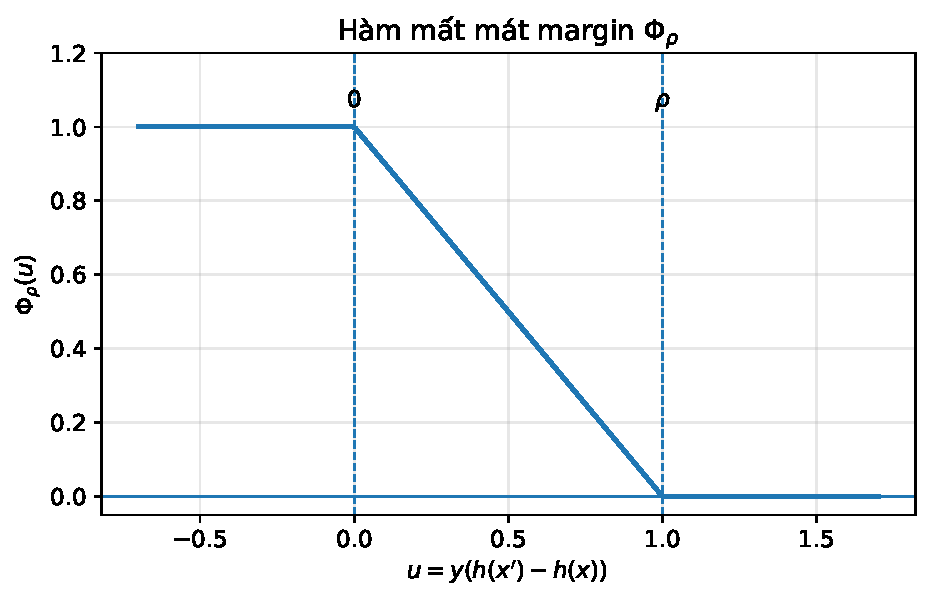
\includegraphics[width=0.82\textwidth]{figures/sec3_margin_loss_phi.pdf}
    \caption{Hàm mất mát margin \(\Phi_{\rho}\). Khi \(u\leq 0\), cặp bị xếp sai hoặc hoà nên bị phạt tối đa. Khi \(0<u<\rho\), cặp đã đúng chiều nhưng margin chưa đủ lớn nên vẫn bị phạt tuyến tính. Khi \(u\geq\rho\), cặp được xem là đúng với độ tin cậy đủ lớn và không bị phạt.}
    \label{fig:section3-margin-loss-phi}
\end{figure}

Hình~\ref{fig:section3-margin-loss-phi} cho thấy vai trò của tham số \(\rho\). Tham số này đặt ra một ngưỡng an toàn cho hiệu điểm giữa hai đối tượng. Nếu margin chỉ vừa lớn hơn \(0\), mô hình tuy xếp đúng nhưng vẫn thiếu chắc chắn; nếu margin vượt qua \(\rho\), mô hình được xem là đã phân biệt cặp đó đủ rõ.

Lỗi margin thực nghiệm được định nghĩa bởi:
\begin{equation}
    \widehat{R}_{\rho}(h)
    =
    \frac{1}{m}
    \sum_{i=1}^{m}
    \Phi_{\rho}
    \left(
        y_i\big(h(x'_i)-h(x_i)\big)
    \right).
    \label{eq:section3-empirical-margin-loss}
\end{equation}
Vì
\[
    \mathbf{1}[u\leq 0]\leq \Phi_{\rho}(u),
\]
nên lỗi thực nghiệm dạng chỉ thị luôn được chặn trên bởi lỗi margin:
\[
    \widehat{R}(h)\leq \widehat{R}_{\rho}(h).
\]
Điều này cho phép ta phân tích ranking thông qua một hàm mất mát mềm hơn và thuận tiện hơn cho việc xây dựng chặn tổng quát hoá.

\subsection{Rademacher complexity}

Để đo độ phức tạp của lớp giả thuyết \(\mathcal{H}\), ta sử dụng Rademacher complexity. Trực giác, Rademacher complexity đo khả năng một lớp hàm có thể khớp với nhiễu ngẫu nhiên. Một lớp hàm có độ phức tạp cao thường dễ overfit hơn.

Với một mẫu \(S=(z_1,\ldots,z_m)\), empirical Rademacher complexity của một lớp hàm \(\mathcal{G}\) được định nghĩa là:
\begin{equation}
    \widehat{\mathfrak{R}}_{S}(\mathcal{G})
    =
    \mathbb{E}_{\sigma}
    \left[
        \sup_{g\in\mathcal{G}}
        \frac{1}{m}
        \sum_{i=1}^{m}
        \sigma_i g(z_i)
    \right],
    \label{eq:section3-empirical-rademacher}
\end{equation}
trong đó \(\sigma_1,\ldots,\sigma_m\) là các biến Rademacher độc lập, nhận giá trị \(+1\) hoặc \(-1\) với xác suất bằng nhau.

Trong bài toán ranking, mỗi mẫu là một cặp \((x_i,x'_i)\). Ta ký hiệu \(D_1\) là phân phối biên của phần tử thứ nhất \(x\), và \(D_2\) là phân phối biên của phần tử thứ hai \(x'\). Tương ứng, ta xét hai đại lượng:
\[
    \mathfrak{R}^{D_1}_m(\mathcal{H}),
    \qquad
    \mathfrak{R}^{D_2}_m(\mathcal{H}).
\]
Hai đại lượng này xuất hiện trong chặn tổng quát hoá vì hàm điểm được đánh giá trên cả hai phần tử của mỗi cặp.

\subsection{Định lý chặn margin cho ranking}

Ta phát biểu kết quả chặn tổng quát hoá chính cho score-based ranking.

\paragraph{Định lý 3.1.}
Cho \(\mathcal{H}\) là một lớp các hàm thực trên \(\mathcal{X}\). Cố định \(\rho>0\). Khi đó, với mọi \(\delta>0\), với xác suất ít nhất \(1-\delta\) theo việc chọn mẫu \(S\) kích thước \(m\), bất đẳng thức sau đúng đồng thời với mọi \(h\in\mathcal{H}\):
\begin{equation}
    R(h)
    \leq
    \widehat{R}_{\rho}(h)
    +
    \frac{2}{\rho}
    \left(
        \mathfrak{R}^{D_1}_m(\mathcal{H})
        +
        \mathfrak{R}^{D_2}_m(\mathcal{H})
    \right)
    +
    \sqrt{
        \frac{\log(1/\delta)}{2m}
    }.
    \label{eq:section3-margin-bound-expected}
\end{equation}

Ngoài ra, ta cũng có dạng chặn theo empirical Rademacher complexity:
\begin{equation}
    R(h)
    \leq
    \widehat{R}_{\rho}(h)
    +
    \frac{2}{\rho}
    \left(
        \widehat{\mathfrak{R}}_{S_1}(\mathcal{H})
        +
        \widehat{\mathfrak{R}}_{S_2}(\mathcal{H})
    \right)
    +
    3
    \sqrt{
        \frac{\log(2/\delta)}{2m}
    }.
    \label{eq:section3-margin-bound-empirical}
\end{equation}

\begin{figure}[H]
    \centering
    \begin{tikzpicture}[>=Stealth, node distance=0.9cm]
        \node[draw, rounded corners, fill=gray!10, align=center, minimum width=3.3cm, minimum height=1.2cm] (train)
        {\(\widehat{R}_{\rho}(h)\)\\ lỗi margin thực nghiệm};
        \node[draw, rounded corners, fill=gray!10, align=center, minimum width=3.8cm, minimum height=1.2cm, right=of train] (complex)
        {\(\dfrac{2}{\rho}(\mathfrak{R}^{D_1}_m+\mathfrak{R}^{D_2}_m)\)\\ độ phức tạp mô hình};
        \node[draw, rounded corners, fill=gray!10, align=center, minimum width=3.3cm, minimum height=1.2cm, right=of complex] (conf)
        {\(\sqrt{\dfrac{\log(1/\delta)}{2m}}\)\\ độ tin cậy};
        \node[draw, rounded corners, fill=gray!20, align=center, minimum width=3.3cm, minimum height=1.2cm, below=1.4cm of complex] (gen)
        {\(R(h)\)\\ lỗi tổng quát};
        \draw[->, thick] (train.south) -- (gen.north west);
        \draw[->, thick] (complex.south) -- (gen.north);
        \draw[->, thick] (conf.south) -- (gen.north east);
    \end{tikzpicture}
    \caption{Ba thành phần trong chặn tổng quát hoá: lỗi trên tập huấn luyện, độ phức tạp của lớp giả thuyết và sai số do lấy mẫu hữu hạn.}
    \label{fig:section3-margin-bound-components}
\end{figure}

Chặn trên gồm ba thành phần. Thành phần thứ nhất là lỗi margin thực nghiệm \(\widehat{R}_{\rho}(h)\). Thành phần thứ hai phụ thuộc vào độ phức tạp của lớp giả thuyết \(\mathcal{H}\). Thành phần thứ ba phụ thuộc vào kích thước mẫu \(m\) và mức tin cậy \(\delta\).

Định lý cho thấy để lỗi tổng quát \(R(h)\) nhỏ, ta cần đồng thời giảm lỗi margin thực nghiệm và kiểm soát độ phức tạp của lớp giả thuyết. Tham số \(\rho\) tạo ra một sự đánh đổi: nếu \(\rho\) lớn, yêu cầu margin nghiêm ngặt hơn nên lỗi margin thực nghiệm có thể tăng; nếu \(\rho\) nhỏ, hệ số \(1/\rho\) trong thành phần độ phức tạp lại tăng.

\subsection{Chứng minh Định lý 3.1}

Đặt \(z=((x,x'),y)\) và định nghĩa lớp hàm margin theo cặp:
\[
    \mathcal{H}_{\Delta}
    =
    \left\{
        ((x,x'),y)
        \mapsto
        y\big(h(x')-h(x)\big)
        \mid
        h\in\mathcal{H}
    \right\}.
\]
Với mỗi \(h\in\mathcal{H}\), nếu một cặp bị xếp sai thì
\[
    y(h(x')-h(x))\leq 0.
\]
Do \(\mathbf{1}[u\leq 0]\leq \Phi_{\rho}(u)\), ta có
\[
    R(h)
    =
    \mathbb{E}_{z}
    \mathbf{1}
    \left[
        y(h(x')-h(x))\leq 0
    \right]
    \leq
    \mathbb{E}_{z}
    \Phi_{\rho}
    \left(
        y(h(x')-h(x))
    \right).
\]
Vì vậy, chỉ cần chặn sai khác giữa kỳ vọng thật và trung bình thực nghiệm của lớp hàm sau:
\[
    \Phi_{\rho}\circ\mathcal{H}_{\Delta}
    =
    \left\{
        ((x,x'),y)
        \mapsto
        \Phi_{\rho}
        \left(
            y\big(h(x')-h(x)\big)
        \right)
        \mid
        h\in\mathcal{H}
    \right\}.
\]

Lớp \(\Phi_{\rho}\circ\mathcal{H}_{\Delta}\) nhận giá trị trong \([0,1]\). Áp dụng chặn tổng quát hoá bằng Rademacher complexity cho lớp hàm bị chặn, với xác suất ít nhất \(1-\delta\), đồng thời với mọi \(h\in\mathcal{H}\):
\[
    \mathbb{E}_{z}
    \Phi_{\rho}
    \left(
        y(h(x')-h(x))
    \right)
    \leq
    \widehat{R}_{\rho}(h)
    +
    2
    \mathfrak{R}_m
    \left(
        \Phi_{\rho}\circ\mathcal{H}_{\Delta}
    \right)
    +
    \sqrt{
        \frac{\log(1/\delta)}{2m}
    }.
\]
Kết hợp với bất đẳng thức \(R(h)\leq \mathbb{E}_{z}\Phi_{\rho}(y(h(x')-h(x)))\), ta được bước chặn đầu tiên.

Tiếp theo, ta chặn độ phức tạp của lớp \(\Phi_{\rho}\circ\mathcal{H}_{\Delta}\). Hàm \(\Phi_{\rho}\) là \(1/\rho\)-Lipschitz. Khi áp dụng định lý contraction, việc cộng một hằng số vào hàm mất mát không làm thay đổi Rademacher complexity vì
\[
    \mathbb{E}_{\sigma}
    \left[
        \frac{1}{m}
        \sum_{i=1}^{m}
        \sigma_i c
    \right]
    =
    0.
\]
Do đó:
\[
    \mathfrak{R}_m
    \left(
        \Phi_{\rho}\circ\mathcal{H}_{\Delta}
    \right)
    \leq
    \frac{1}{\rho}
    \mathfrak{R}_m(\mathcal{H}_{\Delta}).
\]

Ta còn cần chặn \(\mathfrak{R}_m(\mathcal{H}_{\Delta})\) theo độ phức tạp của \(\mathcal{H}\). Với một mẫu \(S=\{((x_i,x'_i),y_i)\}_{i=1}^{m}\), ta có:
\[
\begin{aligned}
    \widehat{\mathfrak{R}}_{S}(\mathcal{H}_{\Delta})
    &=
    \mathbb{E}_{\sigma}
    \left[
        \sup_{h\in\mathcal{H}}
        \frac{1}{m}
        \sum_{i=1}^{m}
        \sigma_i y_i
        \big(h(x'_i)-h(x_i)\big)
    \right] \\
    &\leq
    \mathbb{E}_{\sigma}
    \left[
        \sup_{h\in\mathcal{H}}
        \frac{1}{m}
        \sum_{i=1}^{m}
        \sigma_i y_i h(x'_i)
    \right]
    +
    \mathbb{E}_{\sigma}
    \left[
        \sup_{h\in\mathcal{H}}
        \frac{1}{m}
        \sum_{i=1}^{m}
        (-\sigma_i y_i) h(x_i)
    \right].
\end{aligned}
\]
Vì \(y_i\in\{-1,+1\}\), các biến \(\sigma_i y_i\) và \(-\sigma_i y_i\) vẫn là các biến Rademacher độc lập. Lấy kỳ vọng theo mẫu, hạng thứ nhất trở thành \(\mathfrak{R}^{D_2}_m(\mathcal{H})\), còn hạng thứ hai trở thành \(\mathfrak{R}^{D_1}_m(\mathcal{H})\). Suy ra:
\[
    \mathfrak{R}_m(\mathcal{H}_{\Delta})
    \leq
    \mathfrak{R}^{D_1}_m(\mathcal{H})
    +
    \mathfrak{R}^{D_2}_m(\mathcal{H}).
\]
Thay hai chặn trên vào bất đẳng thức tổng quát hoá, ta thu được:
\[
    R(h)
    \leq
    \widehat{R}_{\rho}(h)
    +
    \frac{2}{\rho}
    \left(
        \mathfrak{R}^{D_1}_m(\mathcal{H})
        +
        \mathfrak{R}^{D_2}_m(\mathcal{H})
    \right)
    +
    \sqrt{
        \frac{\log(1/\delta)}{2m}
    },
\]
đúng đồng thời với mọi \(h\in\mathcal{H}\). Đây chính là dạng chặn theo Rademacher complexity kỳ vọng.

Để thu được dạng empirical Rademacher complexity, ta dùng chặn chuẩn liên hệ giữa độ phức tạp kỳ vọng và độ phức tạp thực nghiệm. Cụ thể, với xác suất cao, mỗi đại lượng \(\mathfrak{R}^{D_j}_m(\mathcal{H})\) có thể được thay bởi \(\widehat{\mathfrak{R}}_{S_j}(\mathcal{H})\) cộng thêm một sai số lấy mẫu bậc \(\sqrt{\log(1/\delta)/m}\). Áp dụng bất đẳng thức này cho hai phân phối biên \(D_1,D_2\) và dùng union bound cho các biến cố xác suất, các hạng sai số được gom lại thành
\[
    3
    \sqrt{
        \frac{\log(2/\delta)}{2m}
    }.
\]
Do đó, với xác suất ít nhất \(1-\delta\), đồng thời với mọi \(h\in\mathcal{H}\):
\[
    R(h)
    \leq
    \widehat{R}_{\rho}(h)
    +
    \frac{2}{\rho}
    \left(
        \widehat{\mathfrak{R}}_{S_1}(\mathcal{H})
        +
        \widehat{\mathfrak{R}}_{S_2}(\mathcal{H})
    \right)
    +
    3
    \sqrt{
        \frac{\log(2/\delta)}{2m}
    }.
\]
Vậy cả hai bất đẳng thức trong Định lý 3.1 đều được chứng minh.

\subsection{[MỞ RỘNG] Giải thích bước Lipschitz của \texorpdfstring{\(\Phi_{\rho}\)}{Phi rho}}

Từ định nghĩa của \(\Phi_{\rho}\), ta thấy hàm này là hằng số trên \((-\infty,0]\), giảm tuyến tính trên \((0,\rho)\), và lại là hằng số trên \([\rho,+\infty)\). Trên đoạn giữa, độ dốc của hàm là
\[
    -\frac{1}{\rho}.
\]
Do đó, với mọi \(u,v\in\mathbb{R}\), ta có:
\[
    |\Phi_{\rho}(u)-\Phi_{\rho}(v)|
    \leq
    \frac{1}{\rho}|u-v|.
\]
Vì vậy, \(\Phi_{\rho}\) là hàm \(1/\rho\)-Lipschitz. Đây là lý do trong bước contraction, Rademacher complexity của lớp sau khi ghép với \(\Phi_{\rho}\) được nhân với hệ số \(1/\rho\). Trực quan từ Hình~\ref{fig:section3-margin-loss-phi}, độ dốc lớn nhất về trị tuyệt đối của đồ thị chính là \(1/\rho\).

\subsection{Hệ quả cho lớp hàm kernel}

Một hệ quả quan trọng của Định lý 3.1 là chặn tổng quát hoá cho lớp hàm kernel. Giả sử \(K:\mathcal{X}\times\mathcal{X}\rightarrow\mathbb{R}\) là một kernel xác định dương, \(\Phi:\mathcal{X}\rightarrow\mathcal{F}\) là ánh xạ đặc trưng tương ứng, và xét lớp giả thuyết:
\[
    \mathcal{H}
    =
    \left\{
        x\mapsto w\cdot \Phi(x)
        \mid
        \|w\|_{\mathcal{F}}\leq \Lambda
    \right\}.
\]
Đặt
\[
    r=\sup_{x\in\mathcal{X}}K(x,x).
\]
Khi đó, với xác suất ít nhất \(1-\delta\), với mọi \(h\in\mathcal{H}\), ta có:
\begin{equation}
    R(h)
    \leq
    \widehat{R}_{\rho}(h)
    +
    4
    \sqrt{
        \frac{r^2\Lambda^2}{\rho^2 m}
    }
    +
    \sqrt{
        \frac{\log(1/\delta)}{2m}
    }.
    \label{eq:section3-kernel-margin-bound}
\end{equation}

Chặn này đáng chú ý vì nó không phụ thuộc trực tiếp vào số chiều của không gian đặc trưng \(\mathcal{F}\). Thay vào đó, nó phụ thuộc vào margin \(\rho\), kích thước mẫu \(m\), cận \(r\) của kernel và chuẩn của vector trọng số thông qua \(\Lambda\).

\subsection{[MỞ RỘNG] Phân tích độ phức tạp của score-based ranking}

Ranking theo từng cặp có thể tốn kém vì số lượng cặp tăng nhanh theo số đối tượng. Nếu có \(n\) đối tượng và xét tất cả các cặp không lặp, số lượng cặp là:
\begin{equation}
    |\mathcal{P}|
    =
    \binom{n}{2}
    =
    \frac{n(n-1)}{2}
    =
    O(n^2).
    \label{eq:section3-number-of-pairs}
\end{equation}

\begin{figure}[H]
    \centering
    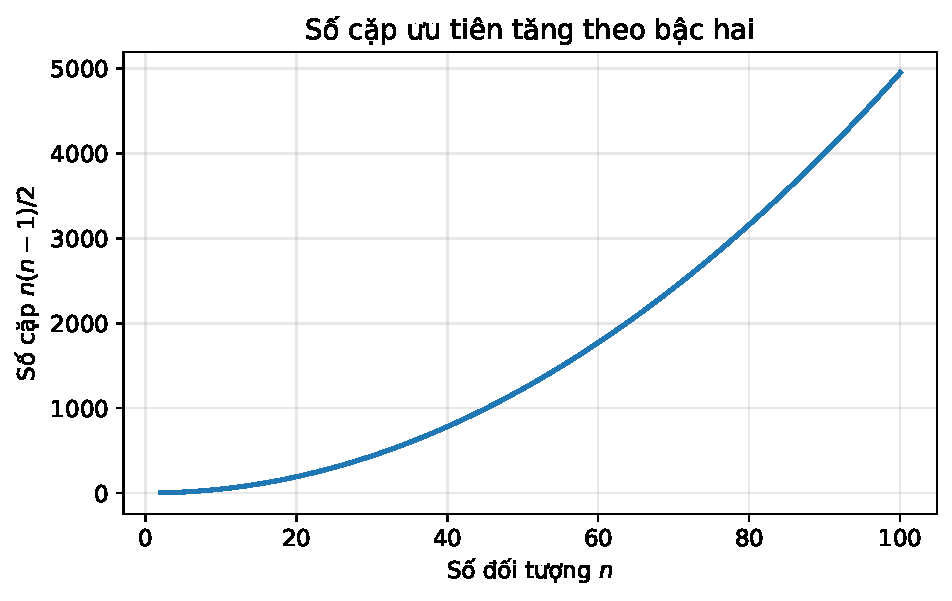
\includegraphics[width=0.82\textwidth]{figures/sec3_pair_count_complexity.pdf}
    \caption{Số cặp ưu tiên tăng theo bậc hai khi số đối tượng \(n\) tăng. Với \(n=100\), nếu xét toàn bộ các cặp không lặp thì có \(\binom{100}{2}=4950\) cặp.}
    \label{fig:section3-pair-count-complexity}
\end{figure}

Hình~\ref{fig:section3-pair-count-complexity} minh hoạ vì sao pairwise ranking có thể nhanh chóng trở nên tốn kém khi \(n\) lớn. Chỉ cần tăng số đối tượng, số cặp cần xét tăng nhanh hơn nhiều so với \(n\). Đây là lý do các hệ thống ranking thực tế thường không huấn luyện trên toàn bộ mọi cặp có thể, mà dùng lấy mẫu cặp, mini-batch hoặc các kỹ thuật tối ưu chuyên biệt.

Với mô hình tuyến tính \(h_w(x)=w^\top x\), chi phí tính điểm cho \(n\) đối tượng là \(O(nd)\), và chi phí sắp xếp để tạo ranking là \(O(n\log n)\). Do đó, chi phí suy luận là:
\[
    O(nd+n\log n).
\]
Nếu huấn luyện trực tiếp trên toàn bộ các cặp, mỗi cặp cần tính hiệu điểm
\[
    h_w(x_j)-h_w(x_i)=w^\top(x_j-x_i),
\]
có chi phí \(O(d)\). Vì vậy, chi phí cho một epoch huấn luyện là:
\[
    O(n^2d).
\]

\begin{table}[H]
    \centering
    \begin{tabular}{lll}
        \toprule
        \textbf{Bước xử lý} & \textbf{Chi phí} & \textbf{Ý nghĩa} \\
        \midrule
        Tính điểm cho \(n\) đối tượng & \(O(nd)\) & Tính \(h_w(x)=w^\top x\) \\
        Sắp xếp để tạo ranking & \(O(n\log n)\) & Xếp đối tượng theo điểm giảm dần \\
        Tạo toàn bộ cặp & \(O(n^2)\) & Số cặp tăng theo \(\binom{n}{2}\) \\
        Một epoch pairwise training & \(O(n^2d)\) & Tính loss/gradient trên mọi cặp \\
        \bottomrule
    \end{tabular}
    \caption{Tóm tắt độ phức tạp của score-based pairwise ranking với mô hình tuyến tính.}
    \label{tab:section3-complexity-summary}
\end{table}

\subsection{Ví dụ minh hoạ về margin}

Xét ba tài liệu \(d_1,d_2,d_3\) với thứ tự đúng:
\[
    d_1 \succ d_2 \succ d_3.
\]
Giả sử mô hình dự đoán điểm:
\[
    h(d_1)=2.0,
    \qquad
    h(d_2)=1.2,
    \qquad
    h(d_3)=1.1.
\]

\begin{figure}[H]
    \centering
    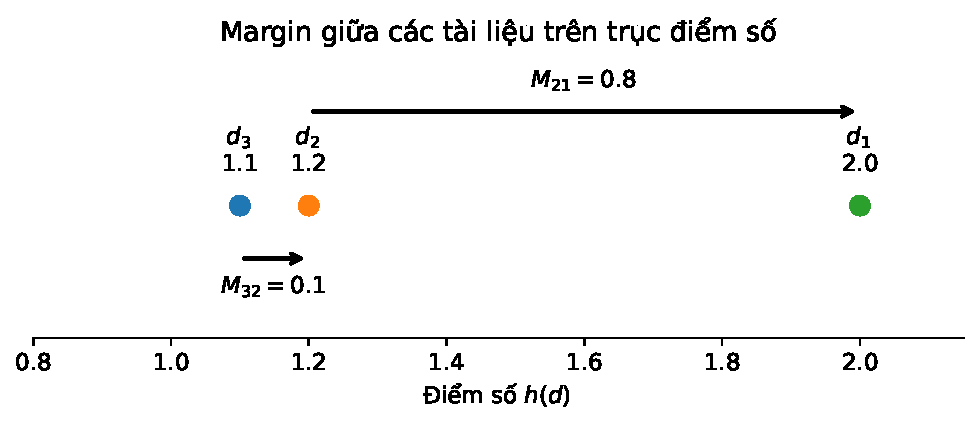
\includegraphics[width=0.86\textwidth]{figures/sec3_margin_on_score_axis.pdf}
    \caption{Minh hoạ margin giữa các tài liệu trên trục điểm số. Cặp \((d_2,d_1)\) có margin lớn hơn, trong khi cặp \((d_3,d_2)\) có margin nhỏ nên kém chắc chắn hơn dù vẫn được xếp đúng.}
    \label{fig:section3-margin-on-score-axis}
\end{figure}

Với cặp \((d_2,d_1)\), margin là:
\[
    M_{21}(h)
    =
    h(d_1)-h(d_2)
    =
    0.8.
\]
Với cặp \((d_3,d_2)\), margin là:
\[
    M_{32}(h)
    =
    h(d_2)-h(d_3)
    =
    0.1.
\]
Cả hai cặp đều được xếp đúng vì margin dương. Tuy nhiên, Hình~\ref{fig:section3-margin-on-score-axis} cho thấy hai trường hợp này không có cùng mức độ chắc chắn. Cặp \((d_2,d_1)\) có khoảng cách điểm lớn, còn cặp \((d_3,d_2)\) chỉ cách nhau \(0.1\), nên dễ bị đảo thứ tự nếu điểm dự đoán có nhiễu nhỏ.

Nếu chọn \(\rho=0.5\), cặp \((d_3,d_2)\) vẫn bị phạt bởi margin loss vì margin chỉ bằng \(0.1\), nhỏ hơn \(\rho\):
\[
    \Phi_{0.5}(0.1)
    =
    1-\frac{0.1}{0.5}
    =
    0.8.
\]
Ví dụ này cho thấy margin loss không chỉ quan tâm đến việc xếp đúng hay sai, mà còn quan tâm đến mức độ chắc chắn của thứ tự được dự đoán.

\subsection{Tóm tắt}

Phần này đã trình bày thiết lập score-based ranking, trong đó mô hình học một hàm điểm \(h:\mathcal{X}\rightarrow\mathbb{R}\) và dùng hàm này để sinh thứ tự xếp hạng. Ta đã định nghĩa lỗi tổng quát, lỗi thực nghiệm, margin theo cặp và lỗi margin thực nghiệm. Kết quả chính là chặn tổng quát hoá dựa trên Rademacher complexity, cho thấy lỗi ranking có thể được kiểm soát thông qua lỗi margin thực nghiệm và độ phức tạp của lớp giả thuyết.

Các hình minh hoạ trong phần này giúp làm rõ ba ý chính. Thứ nhất, \(\Phi_{\rho}\) là một surrogate loss mềm hơn lỗi chỉ thị và phạt cả các cặp đúng nhưng margin nhỏ. Thứ hai, margin có thể được hiểu trực quan là khoảng cách điểm giữa hai đối tượng trên trục score. Thứ ba, số lượng cặp trong pairwise ranking tăng theo \(O(n^2)\), khiến việc huấn luyện trực tiếp trên toàn bộ cặp trở nên tốn kém với dữ liệu lớn.

Các kết quả trên cũng giải thích vì sao các thuật toán ranking dựa trên margin thường tìm một hàm điểm vừa có lỗi margin nhỏ, vừa có độ phức tạp được kiểm soát. Đây là cơ sở tự nhiên dẫn đến các phương pháp như Ranking SVM ở phần tiếp theo.

\section{Ranking với Support Vector Machines}

Phần trước đã trình bày chặn tổng quát hoá dựa trên margin cho score-based ranking. Chặn này gợi ý một nguyên lý thiết kế thuật toán tự nhiên: tìm một hàm điểm có lỗi margin thực nghiệm nhỏ, đồng thời kiểm soát độ phức tạp của lớp giả thuyết. Trong phần này, ta trình bày thuật toán ranking dựa trên Support Vector Machines, thường được gọi là \textit{SVM-ranking} hoặc \textit{Ranking SVM}.

Ý tưởng chính của SVM-ranking là biến bài toán ranking theo từng cặp thành một bài toán phân loại nhị phân trên các vector hiệu. Thay vì học trực tiếp từ từng điểm \(x\), thuật toán học từ các cặp \((x_i,x'_i)\) bằng cách xét hiệu đặc trưng giữa hai đối tượng.

\subsection{Từ chặn margin đến bài toán tối ưu}

Trong score-based ranking, ta xét lớp giả thuyết kernel:
\[
    \mathcal{H}
    =
    \left\{
        x\mapsto w\cdot \Phi(x)
        \mid
        \|w\|_{\mathcal{F}}\leq \Lambda
    \right\},
\]
trong đó \(\Phi:\mathcal{X}\rightarrow\mathcal{F}\) là ánh xạ đặc trưng tương ứng với kernel \(K\), còn \(w\in\mathcal{F}\) là vector tham số.

Với một cặp huấn luyện \((x_i,x'_i,y_i)\), margin ranking là:
\[
    y_i
    \left(
        h_w(x'_i)-h_w(x_i)
    \right)
    =
    y_i
    w\cdot
    \left(
        \Phi(x'_i)-\Phi(x_i)
    \right).
\]

Do đó, điều kiện một cặp được xếp đúng với margin ít nhất \(1\) là:
\begin{equation}
    y_i
    w\cdot
    \left(
        \Phi(x'_i)-\Phi(x_i)
    \right)
    \geq 1.
    \label{eq:section4-hard-margin-ranking}
\end{equation}

Trong thực tế, dữ liệu ranking thường không thể được xếp đúng hoàn toàn với margin \(1\). Vì vậy, ta đưa vào các biến slack \(\xi_i\geq 0\), cho phép một số cặp vi phạm điều kiện margin:
\begin{equation}
    y_i
    w\cdot
    \left(
        \Phi(x'_i)-\Phi(x_i)
    \right)
    \geq
    1-\xi_i,
    \qquad
    i=1,\ldots,m.
    \label{eq:section4-soft-margin-ranking}
\end{equation}

Biến \(\xi_i\) đo mức độ vi phạm margin của cặp thứ \(i\). Nếu \(\xi_i=0\), cặp đó đạt margin ít nhất \(1\); nếu \(\xi_i>0\), cặp đó vi phạm một phần hoặc toàn bộ điều kiện margin.

\subsection{Bài toán tối ưu primal của SVM-ranking}

Từ các điều kiện trên, bài toán tối ưu primal của SVM-ranking được viết dưới dạng:
\begin{equation}
    \min_{w,\xi}
    \quad
    \frac{1}{2}\|w\|_{\mathcal{F}}^2
    +
    C
    \sum_{i=1}^{m}
    \xi_i,
    \label{eq:section4-ranking-svm-primal}
\end{equation}
với các ràng buộc:
\[
    y_i
    w\cdot
    \left(
        \Phi(x'_i)-\Phi(x_i)
    \right)
    \geq
    1-\xi_i,
    \qquad
    \xi_i\geq 0,
    \qquad
    i=1,\ldots,m.
\]

Trong hàm mục tiêu~\eqref{eq:section4-ranking-svm-primal}, thành phần \(\frac{1}{2}\|w\|_{\mathcal{F}}^2\) kiểm soát độ phức tạp của mô hình, còn \(C\sum_i \xi_i\) đo tổng mức độ vi phạm margin trên tập huấn luyện. Tham số \(C>0\) điều chỉnh sự đánh đổi giữa margin lớn và lỗi huấn luyện nhỏ.

Nếu \(C\) lớn, thuật toán ưu tiên giảm lỗi huấn luyện. Nếu \(C\) nhỏ, thuật toán ưu tiên nghiệm có chuẩn nhỏ hơn, tức là mô hình đơn giản hơn, nhưng có thể chấp nhận nhiều vi phạm margin hơn.

\subsection{Liên hệ với pairwise hinge loss}

Bài toán tối ưu trên có thể được viết dưới dạng tối thiểu hoá regularized pairwise hinge loss. Với một cặp \((x_i,x'_i,y_i)\), pairwise hinge loss là:
\begin{equation}
    \ell_i(w)
    =
    \max
    \left(
        0,
        1
        -
        y_i
        w\cdot
        \left(
            \Phi(x'_i)-\Phi(x_i)
        \right)
    \right).
    \label{eq:section4-pairwise-hinge-loss}
\end{equation}

Khi đó, bài toán SVM-ranking tương đương với:
\begin{equation}
    \min_w
    \quad
    \frac{1}{2}\|w\|_{\mathcal{F}}^2
    +
    C
    \sum_{i=1}^{m}
    \max
    \left(
        0,
        1
        -
        y_i
        w\cdot
        \left(
            \Phi(x'_i)-\Phi(x_i)
        \right)
    \right).
    \label{eq:section4-regularized-pairwise-hinge}
\end{equation}

Công thức~\eqref{eq:section4-regularized-pairwise-hinge} cho thấy SVM-ranking không tối ưu trực tiếp lỗi pairwise misranking dạng chỉ thị, mà tối ưu một hàm mất mát lồi thay thế là pairwise hinge loss.

\subsection{Ranking như một bài toán SVM trên vector hiệu}

Điểm quan trọng của SVM-ranking là bài toán ranking có thể được xem như một bài toán SVM thông thường trên không gian các vector hiệu. Định nghĩa ánh xạ:
\begin{equation}
    \Psi(x,x')
    =
    \Phi(x')-\Phi(x).
    \label{eq:section4-pairwise-feature-map}
\end{equation}

Khi đó, điều kiện margin trở thành:
\[
    y_i
    w\cdot
    \Psi(x_i,x'_i)
    \geq
    1-\xi_i.
\]

Đây chính là dạng ràng buộc quen thuộc của soft-margin SVM trong classification, với mỗi mẫu huấn luyện mới là:
\[
    \left(
        \Psi(x_i,x'_i),
        y_i
    \right).
\]

Như vậy, SVM-ranking không phải là một thuật toán hoàn toàn tách biệt với SVM. Nó là một trường hợp đặc biệt của SVM, trong đó đặc trưng của một mẫu là hiệu đặc trưng giữa hai đối tượng cần so sánh.

\subsection{Hình học của SVM-ranking}

Sau phép biến đổi \(\Psi(x,x')=\Phi(x')-\Phi(x)\), mỗi cặp đối tượng trở thành một điểm trong không gian vector hiệu. Trong không gian này, SVM-ranking tìm một siêu phẳng phân tách các vector hiệu có nhãn \(+1\) và \(-1\), tương tự SVM phân loại nhị phân.

Siêu phẳng \(w^\top z=0\), với \(z=\Psi(x,x')\), quyết định xem mô hình xếp \(x'\) cao hơn \(x\) hay ngược lại. Nếu
\[
    w^\top \Psi(x,x')>0,
\]
thì mô hình có xu hướng xếp \(x'\) cao hơn \(x\). Ngược lại, nếu giá trị này âm, mô hình xếp \(x\) cao hơn \(x'\).

Góc nhìn hình học này cho thấy SVM-ranking thực chất là việc học một siêu phẳng phân tách trong không gian các quan hệ so sánh.

\subsection{Dạng dual và kernel cho ranking}

Vì SVM-ranking có thể được xem là SVM trên vector hiệu, ta có thể sử dụng kernel trick. Kernel trên các cặp được xác định thông qua tích vô hướng:
\[
    K'_{ij}
    =
    \Psi(x_i,x'_i)
    \cdot
    \Psi(x_j,x'_j).
\]

Thay định nghĩa \(\Psi(x,x')=\Phi(x')-\Phi(x)\), ta có:
\begin{equation}
\begin{aligned}
    K'_{ij}
    &=
    \left(
        \Phi(x'_i)-\Phi(x_i)
    \right)
    \cdot
    \left(
        \Phi(x'_j)-\Phi(x_j)
    \right)\\
    &=
    K(x'_i,x'_j)
    -
    K(x'_i,x_j)
    -
    K(x_i,x'_j)
    +
    K(x_i,x_j).
\end{aligned}
    \label{eq:section4-pairwise-kernel}
\end{equation}

Tương đương, công thức trên có thể viết là:
\[
    K'_{ij}
    =
    K(x_i,x_j)
    +
    K(x'_i,x'_j)
    -
    K(x'_i,x_j)
    -
    K(x_i,x'_j).
\]

Công thức~\eqref{eq:section4-pairwise-kernel} cho thấy ta không cần tính trực tiếp ánh xạ \(\Phi\). Chỉ cần có kernel \(K\) giữa các đối tượng ban đầu, ta có thể xây dựng kernel \(K'\) giữa các cặp đối tượng.

\subsection{Chứng minh liên hệ giữa SVM-ranking và SVM chuẩn}

Ta trình bày ngắn gọn liên hệ giữa SVM-ranking và SVM chuẩn. Với mỗi cặp \((x_i,x'_i)\), định nghĩa mẫu mới:
\[
    z_i
    =
    \Psi(x_i,x'_i)
    =
    \Phi(x'_i)-\Phi(x_i).
\]

Khi đó, ràng buộc của SVM-ranking:
\[
    y_i
    w\cdot
    \left(
        \Phi(x'_i)-\Phi(x_i)
    \right)
    \geq
    1-\xi_i
\]
trở thành:
\[
    y_i w\cdot z_i
    \geq
    1-\xi_i.
\]

Đây chính là ràng buộc của soft-margin SVM cho bài toán phân loại nhị phân trên tập mẫu \((z_i,y_i)\). Hàm mục tiêu cũng giữ nguyên dạng:
\[
    \min_{w,\xi}
    \quad
    \frac{1}{2}\|w\|_{\mathcal{F}}^2
    +
    C
    \sum_{i=1}^{m}
    \xi_i.
\]

Do đó, bài toán SVM-ranking tương đương với soft-margin SVM chuẩn sau khi biến đổi mỗi cặp đối tượng thành một vector hiệu. Điều này giải thích vì sao các tính chất của SVM, như kernel trick và margin maximization, có thể được áp dụng trực tiếp cho ranking.

\subsection{Ví dụ minh hoạ}

Xét ba tài liệu \(d_1,d_2,d_3\) với thứ tự đúng:
\[
    d_1 \succ d_2 \succ d_3.
\]

Giả sử mỗi tài liệu được biểu diễn bởi vector hai chiều:
\[
    x_1=
    \begin{bmatrix}
        2\\
        1
    \end{bmatrix},
    \quad
    x_2=
    \begin{bmatrix}
        1\\
        1
    \end{bmatrix},
    \quad
    x_3=
    \begin{bmatrix}
        0\\
        1
    \end{bmatrix}.
\]

Với cặp \((d_2,d_1)\), vì \(d_1\) được ưu tiên hơn \(d_2\), nhãn là \(y_{21}=+1\). Vector hiệu tương ứng là:
\[
    x_1-x_2
    =
    \begin{bmatrix}
        1\\
        0
    \end{bmatrix}.
\]

Nếu mô hình có trọng số
\[
    w=
    \begin{bmatrix}
        1\\
        0
    \end{bmatrix},
\]
thì margin của cặp này là:
\[
    y_{21}w^\top(x_1-x_2)=1.
\]

Cặp này đạt đúng margin \(1\). Ví dụ này cho thấy SVM-ranking học một vector \(w\) sao cho hiệu đặc trưng giữa đối tượng được ưu tiên và đối tượng kém ưu tiên có tích vô hướng dương và đủ lớn với \(w\).

\subsection{[MỞ RỘNG] Phân tích độ phức tạp của SVM-ranking}

SVM-ranking làm việc trên các cặp đối tượng, vì vậy chi phí tính toán phụ thuộc mạnh vào số lượng cặp huấn luyện. Nếu ban đầu có \(n\) đối tượng và tạo tất cả các cặp có thể, số lượng cặp là:
\begin{equation}
    |\mathcal{P}|
    =
    \frac{n(n-1)}{2}
    =
    O(n^2).
    \label{eq:section4-pair-count}
\end{equation}

Nếu mỗi đối tượng có \(d\) đặc trưng, việc tính vector hiệu \(x'_i-x_i\) cho một cặp có chi phí \(O(d)\). Do đó, việc tạo toàn bộ dữ liệu pairwise có chi phí:
\[
    O(n^2d).
\]

Nếu sử dụng kernel, ta cần xây dựng ma trận kernel trên các cặp. Với \(m\) cặp huấn luyện, ma trận kernel \(K'\) có kích thước \(m\times m\), nên chi phí lưu trữ là:
\[
    O(m^2).
\]

Nếu \(m=O(n^2)\), chi phí bộ nhớ trong trường hợp dùng kernel có thể lên tới \(O(n^4)\). Vì vậy, SVM-ranking có thể trở nên rất tốn kém nếu áp dụng trực tiếp cho dữ liệu lớn với toàn bộ các cặp. Trong thực tế, người ta thường dùng lấy mẫu cặp, tối ưu tuyến tính hoặc các thuật toán chuyên biệt cho ranking quy mô lớn.

\subsection{[MỞ RỘNG] So sánh với SVM phân loại nhị phân}

SVM phân loại nhị phân học từ các mẫu riêng lẻ \((x_i,y_i)\), với điều kiện margin:
\[
    y_i w^\top x_i \geq 1-\xi_i.
\]

Trong khi đó, SVM-ranking học từ các cặp \((x_i,x'_i,y_i)\), với điều kiện:
\[
    y_i w^\top(x'_i-x_i)\geq 1-\xi_i.
\]

Hai công thức có cùng cấu trúc. Điểm khác biệt nằm ở biểu diễn đầu vào: SVM phân loại dùng trực tiếp \(x_i\), còn SVM-ranking dùng vector hiệu \(x'_i-x_i\). Vì vậy, có thể xem SVM-ranking là SVM phân loại nhị phân trên không gian các quan hệ so sánh.

Sự khác biệt này cũng phản ánh khác biệt về mục tiêu. SVM phân loại cố gắng dự đoán đúng nhãn của từng điểm, còn SVM-ranking cố gắng dự đoán đúng thứ tự tương đối giữa hai điểm.

\subsection{Hạn chế của SVM-ranking}

Mặc dù SVM-ranking có nền tảng lý thuyết rõ ràng và tận dụng được các công cụ của SVM, phương pháp này có một số hạn chế.

Thứ nhất, số lượng cặp huấn luyện có thể tăng bậc hai theo số đối tượng. Nếu một truy vấn có nhiều tài liệu, việc tạo toàn bộ các cặp tài liệu có thể gây chi phí lớn.

Thứ hai, trong score-based ranking, mô hình học một hàm điểm toàn cục. Hàm điểm này luôn sinh ra một thứ tự bắc cầu. Do đó, nếu quan hệ ưu tiên thật không bắc cầu, không có hàm điểm nào có thể biểu diễn hoàn hảo toàn bộ quan hệ ưu tiên.

Thứ ba, SVM-ranking tối ưu pairwise margin, trong khi nhiều ứng dụng thực tế quan tâm nhiều hơn đến các vị trí đầu danh sách, chẳng hạn top-\(k\) kết quả tìm kiếm. Vì vậy, các độ đo như NDCG, MAP hoặc precision@\(k\) có thể phù hợp hơn trong một số bối cảnh.

\subsection{Tóm tắt}

Phần này đã trình bày thuật toán ranking dựa trên SVM. Từ chặn tổng quát hoá theo margin, ta xây dựng bài toán tối ưu có dạng soft-margin SVM, trong đó mỗi mẫu là một cặp đối tượng và đặc trưng của mẫu là hiệu giữa hai vector đặc trưng. Ánh xạ
\[
    \Psi(x,x')=\Phi(x')-\Phi(x)
\]
cho thấy SVM-ranking thực chất là một trường hợp đặc biệt của SVM chuẩn trên không gian pairwise.

Kết quả này tạo cầu nối giữa lý thuyết ranking và các thuật toán tối ưu margin. Trong phần tiếp theo, ta sẽ nghiên cứu một hướng tiếp cận khác trong score-based ranking: RankBoost.
\section{RankBoost}

Trong các phần trước, ta đã trình bày score-based ranking và thuật toán ranking dựa trên SVM. Một hướng tiếp cận khác trong score-based ranking là sử dụng boosting. Phần này trình bày RankBoost, một thuật toán boosting được thiết kế cho bài toán ranking theo từng cặp.

Tương tự AdaBoost trong phân loại nhị phân, RankBoost kết hợp nhiều mô hình yếu, gọi là \textit{base rankers}, để tạo thành một hàm ranking mạnh hơn. Khác với AdaBoost, RankBoost duy trì phân phối trọng số trên các cặp đối tượng. Các cặp bị xếp sai ở những vòng trước sẽ được tăng trọng số, khiến thuật toán tập trung nhiều hơn vào các cặp khó ở những vòng sau.

\subsection{Thiết lập của RankBoost}

Giả sử tập huấn luyện gồm \(m\) cặp có nhãn:
\[
    S =
    \big((x_1,x'_1,y_1),\ldots,(x_m,x'_m,y_m)\big),
    \qquad
    y_i\in\{-1,0,+1\}.
\]

Theo quy ước, \(y_i=+1\) nghĩa là \(x'_i\) được ưu tiên hơn \(x_i\), \(y_i=-1\) nghĩa là \(x_i\) được ưu tiên hơn \(x'_i\), và \(y_i=0\) nghĩa là hai đối tượng ngang nhau hoặc không có thông tin ưu tiên rõ ràng. Để đơn giản, ta giả sử các cặp có nhãn \(0\) đã được loại bỏ, tức là:
\[
    y_i\neq 0,
    \qquad i=1,\ldots,m.
\]

RankBoost sử dụng một tập các base rankers:
\[
    \mathcal{H}
    =
    \{h:\mathcal{X}\rightarrow\{0,1\}\}.
\]

Mỗi base ranker \(h_t\in\mathcal{H}\) gán cho mỗi đối tượng một giá trị trong \(\{0,1\}\). Sau \(T\) vòng, RankBoost trả về hàm điểm:
\begin{equation}
    g(x)
    =
    \sum_{t=1}^{T}
    \alpha_t h_t(x),
    \label{eq:section5-final-ranker}
\end{equation}
trong đó \(\alpha_t\geq 0\) là trọng số của base ranker \(h_t\). Ranking cuối cùng được sinh ra bằng cách sắp xếp các đối tượng theo giá trị \(g(x)\).

\subsection{Ý tưởng lặp của RankBoost}

RankBoost hoạt động theo từng vòng. Tại vòng \(t\), thuật toán duy trì một phân phối trọng số \(D_t\) trên các cặp huấn luyện. Sau đó, thuật toán chọn một base ranker \(h_t\) tốt đối với phân phối hiện tại, tính trọng số \(\alpha_t\), rồi cập nhật phân phối thành \(D_{t+1}\).

Trực giác của bước cập nhật là: các cặp được xếp đúng sẽ giảm trọng số tương đối, còn các cặp bị xếp sai sẽ tăng trọng số tương đối. Vì vậy, ở các vòng sau, thuật toán tập trung nhiều hơn vào các cặp khó.

\subsection{Phân phối trọng số trên các cặp}

RankBoost duy trì một phân phối \(D_t\) trên các cặp huấn luyện:
\[
    D_t(i)\geq 0,
    \qquad
    \sum_{i=1}^{m}D_t(i)=1.
\]

Ban đầu, mọi cặp được gán trọng số bằng nhau:
\[
    D_1(i)=\frac{1}{m},
    \qquad
    i=1,\ldots,m.
\]

Tại mỗi vòng \(t\), với một cặp \((x_i,x'_i,y_i)\), base ranker \(h_t\) xếp đúng nếu:
\[
    y_i\big(h_t(x'_i)-h_t(x_i)\big)>0.
\]

Nó xếp sai nếu biểu thức trên nhỏ hơn \(0\), và không phân biệt được cặp đó nếu biểu thức bằng \(0\).

\subsection{Các đại lượng \texorpdfstring{\(\epsilon_t^+\), \(\epsilon_t^-\), \(\epsilon_t^0\)}{epsilon}}

Tại vòng \(t\), với phân phối \(D_t\), ta định nghĩa:
\begin{equation}
    \epsilon_t^{+}
    =
    \sum_{i=1}^{m}
    D_t(i)
    \mathbf{1}
    \left[
        y_i\big(h_t(x'_i)-h_t(x_i)\big)=+1
    \right],
    \label{eq:section5-epsilon-plus}
\end{equation}
\begin{equation}
    \epsilon_t^{-}
    =
    \sum_{i=1}^{m}
    D_t(i)
    \mathbf{1}
    \left[
        y_i\big(h_t(x'_i)-h_t(x_i)\big)=-1
    \right],
    \label{eq:section5-epsilon-minus}
\end{equation}
và:
\begin{equation}
    \epsilon_t^{0}
    =
    \sum_{i=1}^{m}
    D_t(i)
    \mathbf{1}
    \left[
        y_i\big(h_t(x'_i)-h_t(x_i)\big)=0
    \right].
    \label{eq:section5-epsilon-zero}
\end{equation}

Ba đại lượng này lần lượt là tổng trọng số của các cặp được xếp đúng, xếp sai và không được phân biệt bởi \(h_t\). Ta có:
\[
    \epsilon_t^{+}
    +
    \epsilon_t^{-}
    +
    \epsilon_t^{0}
    =
    1.
\]

RankBoost chọn base ranker sao cho \(\epsilon_t^{-}-\epsilon_t^{+}\) nhỏ nhất, tức là ưu tiên base ranker có trọng số xếp đúng lớn và trọng số xếp sai nhỏ. Edge của base ranker được định nghĩa là:
\begin{equation}
    \gamma_t
    =
    \frac{\epsilon_t^{+}-\epsilon_t^{-}}{2}.
    \label{eq:section5-edge}
\end{equation}

Nếu \(\gamma_t>0\), base ranker \(h_t\) xếp đúng nhiều hơn xếp sai theo phân phối hiện tại. Đây là điều kiện yếu giúp boosting cải thiện dần qua các vòng.

\subsection{Trọng số của base ranker}

Sau khi chọn được \(h_t\), RankBoost gán cho nó trọng số:
\begin{equation}
    \alpha_t
    =
    \frac{1}{2}
    \log
    \frac{\epsilon_t^{+}}{\epsilon_t^{-}}.
    \label{eq:section5-alpha}
\end{equation}

Nếu \(\epsilon_t^{+}>\epsilon_t^{-}\), thì \(\alpha_t>0\). Base ranker càng tốt, tức là \(\epsilon_t^{+}\) càng lớn so với \(\epsilon_t^{-}\), thì \(\alpha_t\) càng lớn. Vì vậy, các base rankers mạnh hơn sẽ có ảnh hưởng lớn hơn trong hàm điểm cuối cùng \(g\).

\subsection{Cập nhật phân phối trọng số}

Sau khi chọn \(h_t\) và \(\alpha_t\), RankBoost cập nhật phân phối trọng số trên các cặp:
\begin{equation}
    D_{t+1}(i)
    =
    \frac{
        D_t(i)
        \exp
        \left(
            -\alpha_t
            y_i
            \big(h_t(x'_i)-h_t(x_i)\big)
        \right)
    }{
        Z_t
    },
    \label{eq:section5-distribution-update}
\end{equation}
trong đó \(Z_t\) là hệ số chuẩn hoá:
\begin{equation}
    Z_t
    =
    \sum_{i=1}^{m}
    D_t(i)
    \exp
    \left(
        -\alpha_t
        y_i
        \big(h_t(x'_i)-h_t(x_i)\big)
    \right).
    \label{eq:section5-normalization-factor}
\end{equation}

Hệ số \(Z_t\) đảm bảo \(D_{t+1}\) vẫn là một phân phối. Nếu cặp thứ \(i\) được xếp đúng, trọng số của nó được nhân với \(e^{-\alpha_t}\). Nếu cặp đó bị xếp sai, trọng số được nhân với \(e^{\alpha_t}\). Nếu cặp bị hoà, hệ số nhân là \(1\).

Vì \(\alpha_t>0\), các cặp bị xếp sai được tăng trọng số tương đối, còn các cặp được xếp đúng bị giảm trọng số tương đối. Đây là cơ chế giúp RankBoost tập trung vào các cặp khó hơn qua từng vòng.

\subsection{Thuật toán RankBoost}

Thuật toán RankBoost có thể tóm tắt như sau.

\begin{enumerate}[label=\textbf{Bước \arabic*.}, leftmargin=*]
    \item Khởi tạo phân phối đều:
    \[
        D_1(i)=\frac{1}{m},
        \qquad
        i=1,\ldots,m.
    \]

    \item Với mỗi vòng \(t=1,\ldots,T\), chọn base ranker:
    \[
        h_t
        \in
        \arg\min_{h\in\mathcal{H}}
        \left(
            \epsilon_t^{-}(h)-\epsilon_t^{+}(h)
        \right).
    \]

    \item Tính trọng số:
    \[
        \alpha_t
        =
        \frac{1}{2}
        \log
        \frac{\epsilon_t^{+}}{\epsilon_t^{-}}.
    \]

    \item Cập nhật phân phối theo công thức~\eqref{eq:section5-distribution-update}.

    \item Sau \(T\) vòng, trả về:
    \[
        g(x)
        =
        \sum_{t=1}^{T}
        \alpha_t h_t(x).
    \]
\end{enumerate}

Hàm \(g\) sau cùng được dùng để xếp hạng các đối tượng: đối tượng nào có \(g(x)\) lớn hơn sẽ được xếp cao hơn.

\subsection{Biểu diễn phân phối sau nhiều vòng}

Để phân tích RankBoost, ta cần biểu diễn \(D_{t+1}\) theo tổ hợp các base rankers đã chọn. Gọi:
\[
    g_t(x)
    =
    \sum_{s=1}^{t}
    \alpha_s h_s(x).
\]

Khi đó, bằng cách khai triển đệ quy công thức cập nhật, ta có:
\begin{equation}
    D_{t+1}(i)
    =
    \frac{
        \exp
        \left(
            -y_i
            \big(g_t(x'_i)-g_t(x_i)\big)
        \right)
    }{
        m
        \prod_{s=1}^{t}Z_s
    }.
    \label{eq:section5-distribution-closed-form}
\end{equation}

Công thức này cho thấy trọng số của một cặp sau nhiều vòng phụ thuộc vào margin tích luỹ của hàm \(g_t\) trên cặp đó. Nếu cặp có margin lớn và đúng chiều, trọng số giảm; nếu cặp bị xếp sai hoặc margin nhỏ, trọng số vẫn lớn.

\subsection{Chặn lỗi thực nghiệm của RankBoost}

Sau \(T\) vòng, RankBoost trả về:
\[
    g(x)=g_T(x)=\sum_{t=1}^{T}\alpha_t h_t(x).
\]

Lỗi thực nghiệm của \(g\) là:
\begin{equation}
    \widehat{R}(g)
    =
    \frac{1}{m}
    \sum_{i=1}^{m}
    \mathbf{1}
    \left[
        y_i
        \big(g(x'_i)-g(x_i)\big)
        \leq 0
    \right].
    \label{eq:section5-rankboost-empirical-error}
\end{equation}

Ta có chặn lỗi thực nghiệm sau.

\paragraph{Định lý 5.1.}
Lỗi thực nghiệm của hàm \(g\) trả về bởi RankBoost thoả:
\begin{equation}
    \widehat{R}(g)
    \leq
    \exp
    \left(
        -2
        \sum_{t=1}^{T}
        \left(
            \frac{\epsilon_t^{+}-\epsilon_t^{-}}{2}
        \right)^2
    \right).
    \label{eq:section5-rankboost-empirical-bound}
\end{equation}

Nếu tồn tại \(\gamma>0\) sao cho với mọi \(t=1,\ldots,T\),
\[
    \gamma
    \leq
    \frac{\epsilon_t^{+}-\epsilon_t^{-}}{2},
\]
thì:
\begin{equation}
    \widehat{R}(g)
    \leq
    \exp(-2\gamma^2T).
    \label{eq:section5-rankboost-exponential-bound}
\end{equation}

Định lý cho thấy nếu mỗi vòng boosting tìm được một base ranker có edge dương ít nhất \(\gamma\), lỗi thực nghiệm của RankBoost giảm theo hàm mũ theo số vòng \(T\). Đây là tính chất tương tự AdaBoost trong bài toán phân loại nhị phân.

\subsection{Chứng minh Định lý 5.1}

Ta chỉ trình bày ý tưởng chính của chứng minh. Sử dụng bất đẳng thức:
\[
    \mathbf{1}[u\leq 0]\leq \exp(-u),
    \qquad
    \forall u\in\mathbb{R},
\]
với
\[
    u_i=
    y_i
    \big(g(x'_i)-g(x_i)\big),
\]
ta có:
\[
    \widehat{R}(g)
    \leq
    \frac{1}{m}
    \sum_{i=1}^{m}
    \exp
    \left(
        -y_i
        \big(g(x'_i)-g(x_i)\big)
    \right).
\]

Từ công thức~\eqref{eq:section5-distribution-closed-form} với \(t=T\), suy ra:
\[
    \widehat{R}(g)
    \leq
    \prod_{t=1}^{T}Z_t.
\]

Tiếp theo, chia các cặp thành ba nhóm được xếp đúng, xếp sai và hoà, ta có:
\[
    Z_t
    =
    \epsilon_t^{+}e^{-\alpha_t}
    +
    \epsilon_t^{-}e^{\alpha_t}
    +
    \epsilon_t^{0}.
\]

Với lựa chọn
\[
    \alpha_t
    =
    \frac{1}{2}
    \log
    \frac{\epsilon_t^{+}}{\epsilon_t^{-}},
\]
ta thu được:
\[
    Z_t
    =
    2\sqrt{\epsilon_t^{+}\epsilon_t^{-}}
    +
    \epsilon_t^{0}.
\]

Sử dụng các bước chặn chuẩn trong phân tích RankBoost, ta có:
\[
    Z_t
    \leq
    \exp
    \left(
        -2
        \left(
            \frac{\epsilon_t^{+}-\epsilon_t^{-}}{2}
        \right)^2
    \right).
\]

Thay chặn này vào \(\widehat{R}(g)\leq\prod_{t=1}^{T}Z_t\), ta thu được:
\[
    \widehat{R}(g)
    \leq
    \exp
    \left(
        -2
        \sum_{t=1}^{T}
        \left(
            \frac{\epsilon_t^{+}-\epsilon_t^{-}}{2}
        \right)^2
    \right).
\]

Nếu mỗi edge đều không nhỏ hơn \(\gamma\), thì tổng trong mũ không nhỏ hơn \(T\gamma^2\), và do đó:
\[
    \widehat{R}(g)
    \leq
    \exp(-2\gamma^2T).
\]

\subsection{[MỞ RỘNG] Vì sao \texorpdfstring{\(\alpha_t\)}{alpha t} tối thiểu hoá \texorpdfstring{\(Z_t\)}{Zt}}

Hệ số \(\alpha_t\) có thể được giải thích bằng cách xem \(Z_t\) như một hàm của \(\alpha\):
\[
    Z_t(\alpha)
    =
    \epsilon_t^{+}e^{-\alpha}
    +
    \epsilon_t^{-}e^{\alpha}
    +
    \epsilon_t^{0}.
\]

Lấy đạo hàm theo \(\alpha\):
\[
    \frac{dZ_t(\alpha)}{d\alpha}
    =
    -\epsilon_t^{+}e^{-\alpha}
    +
    \epsilon_t^{-}e^{\alpha}.
\]

Cho đạo hàm bằng \(0\), ta được:
\[
    e^{2\alpha}
    =
    \frac{\epsilon_t^{+}}{\epsilon_t^{-}}.
\]

Do đó:
\[
    \alpha
    =
    \frac{1}{2}
    \log
    \frac{\epsilon_t^{+}}{\epsilon_t^{-}}.
\]

Vì vậy, công thức chọn \(\alpha_t\) trong RankBoost được chọn để tối thiểu hoá hệ số chuẩn hoá \(Z_t\), mà tích các \(Z_t\) lại là một chặn trên của lỗi thực nghiệm.

\subsection{RankBoost và coordinate descent}

RankBoost cũng có thể được hiểu như việc áp dụng coordinate descent lên một hàm mục tiêu lồi và khả vi. Xét hàm:
\begin{equation}
    F(\alpha)
    =
    \sum_{i=1}^{m}
    \exp
    \left(
        -y_i
        \left[
            g(x'_i)-g(x_i)
        \right]
    \right),
    \label{eq:section5-coordinate-descent-objective}
\end{equation}
trong đó:
\[
    g(x)
    =
    \sum_{t=1}^{T}
    \alpha_t h_t(x).
\]

Hàm \(F(\alpha)\) là một chặn lồi của lỗi pairwise misranking dạng chỉ thị. Ở mỗi vòng, RankBoost chọn base ranker \(h_t\) tương ứng với một hướng toạ độ làm giảm nhanh nhất hàm \(F\). Sau đó, hệ số \(\alpha_t\) được chọn để tối thiểu hoá \(F\) theo hướng đó. Vì vậy, RankBoost có thể được xem là coordinate descent trong không gian các tổ hợp tuyến tính của base rankers.

\subsection{Ví dụ minh hoạ}

Xét ba tài liệu \(d_1,d_2,d_3\) với thứ tự đúng:
\[
    d_1 \succ d_2 \succ d_3.
\]

Ta xét ba cặp:
\[
    (d_2,d_1,+1),
    \qquad
    (d_3,d_1,+1),
    \qquad
    (d_3,d_2,+1).
\]

Ban đầu, mỗi cặp có trọng số \(1/3\). Giả sử base ranker \(h_1\) cho điểm:
\[
    h_1(d_1)=1,
    \qquad
    h_1(d_2)=1,
    \qquad
    h_1(d_3)=0.
\]

Khi đó, cặp \((d_2,d_1)\) bị hoà vì \(h_1(d_1)-h_1(d_2)=0\), còn hai cặp \((d_3,d_1)\) và \((d_3,d_2)\) được xếp đúng. Vì vậy:
\[
    \epsilon_1^{+}=\frac{2}{3},
    \qquad
    \epsilon_1^{-}=0,
    \qquad
    \epsilon_1^{0}=\frac{1}{3}.
\]

Ví dụ này cho thấy vai trò của ba nhóm cặp: xếp đúng, xếp sai và hoà điểm. Trong trường hợp \(\epsilon_t^{-}=0\), công thức \(\alpha_t=\frac{1}{2}\log(\epsilon_t^{+}/\epsilon_t^{-})\) không xác định hữu hạn; thực tế có thể xử lý bằng làm trơn nhỏ hoặc dừng sớm nếu không còn cặp bị xếp sai.

\subsection{[MỞ RỘNG] Phân tích độ phức tạp của RankBoost}

Giả sử tập huấn luyện có \(m\) cặp và thuật toán chạy trong \(T\) vòng. Nếu bỏ qua chi phí tìm base ranker, việc tính các đại lượng \(\epsilon_t^{+}\), \(\epsilon_t^{-}\), \(\epsilon_t^{0}\) cần duyệt qua \(m\) cặp, nên có chi phí \(O(m)\). Việc cập nhật phân phối \(D_{t+1}\) cũng có chi phí \(O(m)\).

Do đó, chi phí mỗi vòng là:
\[
    O(m),
\]
và sau \(T\) vòng, tổng chi phí là:
\[
    O(Tm).
\]

Nếu \(m\) được tạo từ tất cả các cặp của \(n\) đối tượng, thì:
\[
    m=
    \frac{n(n-1)}{2}
    =
    O(n^2).
\]

Khi đó, chi phí tổng quát có thể trở thành \(O(Tn^2)\), còn bộ nhớ để lưu phân phối trên các cặp là \(O(n^2)\). Điều này cho thấy RankBoost có thể gặp khó khăn khi số lượng cặp rất lớn, và là động lực để xét các phiên bản hiệu quả hơn trong bipartite ranking.

\subsection{Liên hệ với AdaBoost}

RankBoost có quan hệ chặt chẽ với AdaBoost. Cả hai thuật toán đều duy trì một phân phối trọng số, chọn một weak learner tại mỗi vòng, gán trọng số cho weak learner đó và cập nhật phân phối để tập trung vào các mẫu khó.

Điểm khác biệt chính là AdaBoost duy trì trọng số trên từng điểm dữ liệu \((x_i,y_i)\), còn RankBoost duy trì trọng số trên từng cặp \((x_i,x'_i,y_i)\). Vì vậy, AdaBoost cố gắng giảm lỗi phân loại từng điểm, còn RankBoost cố gắng giảm lỗi xếp hạng theo từng cặp.

\subsection{Tóm tắt}

RankBoost là một thuật toán boosting cho bài toán ranking theo từng cặp. Thuật toán duy trì phân phối trọng số trên các cặp huấn luyện, chọn base ranker có khả năng xếp đúng các cặp có trọng số lớn, sau đó cập nhật phân phối để tập trung vào các cặp bị xếp sai. Hàm ranking cuối cùng là tổ hợp tuyến tính của các base rankers.

Kết quả lý thuyết quan trọng của RankBoost là lỗi thực nghiệm giảm theo hàm mũ nếu tại mỗi vòng tồn tại một base ranker có edge dương. Ngoài ra, RankBoost có thể được hiểu như coordinate descent trên một hàm mục tiêu lồi dạng exponential loss. Phân tích này tạo nền tảng cho phần tiếp theo, nơi ta xét trường hợp đặc biệt nhưng rất quan trọng của ranking: bipartite ranking.
\section{Bipartite ranking, ROC và AUC}

Các phần trước đã trình bày score-based ranking trong thiết lập tổng quát, nơi dữ liệu huấn luyện gồm các cặp đối tượng có nhãn ưu tiên. Trong phần này, ta xét một trường hợp đặc biệt nhưng rất quan trọng của ranking, gọi là \textit{bipartite ranking}. Đây là thiết lập trong đó các đối tượng được chia thành hai nhóm: positive và negative. Mục tiêu của mô hình là xếp các đối tượng positive cao hơn các đối tượng negative.

Bipartite ranking có quan hệ chặt chẽ với binary classification, nhưng mục tiêu của hai bài toán khác nhau. Trong binary classification, ta muốn dự đoán đúng nhãn của từng điểm. Trong bipartite ranking, ta muốn tạo ra một thứ tự sao cho các điểm positive đứng trước các điểm negative. Một độ đo phổ biến cho thiết lập này là AUC, tức diện tích dưới đường cong ROC.

\subsection{Thiết lập bipartite ranking}

Gọi \(\mathcal{X}\) là không gian đầu vào. Trong bipartite ranking, tập dữ liệu được chia thành hai lớp rời nhau:
\[
    \mathcal{X}
    =
    \mathcal{X}_{+}
    \cup
    \mathcal{X}_{-},
    \qquad
    \mathcal{X}_{+}
    \cap
    \mathcal{X}_{-}
    =
    \varnothing.
\]

Các phần tử trong \(\mathcal{X}_{+}\) được gọi là positive points, còn các phần tử trong \(\mathcal{X}_{-}\) được gọi là negative points. Mục tiêu là học một hàm điểm
\[
    h:\mathcal{X}\rightarrow\mathbb{R},
\]
sao cho với mọi \(x^{+}\in\mathcal{X}_{+}\) và \(x^{-}\in\mathcal{X}_{-}\), ta mong muốn:
\begin{equation}
    h(x^{+}) > h(x^{-}).
    \label{eq:section6-positive-above-negative}
\end{equation}

Điều kiện trong công thức~\eqref{eq:section6-positive-above-negative} nói rằng điểm positive nên được xếp cao hơn điểm negative. Đây là mục tiêu cốt lõi của bipartite ranking.

\subsection{Lỗi tổng quát trong bipartite ranking}

Gọi \(D_{+}\) là phân phối trên các điểm positive và \(D_{-}\) là phân phối trên các điểm negative. Lỗi tổng quát của một hàm điểm \(h\) được định nghĩa là xác suất một điểm negative được xếp cao hơn một điểm positive:
\begin{equation}
    R(h)
    =
    \Pr_{\substack{x^{+}\sim D_{+}\\x^{-}\sim D_{-}}}
    \left[
        h(x^{+}) < h(x^{-})
    \right].
    \label{eq:section6-bipartite-generalization-error}
\end{equation}

Công thức này đo trực tiếp lỗi ranking theo từng cặp positive-negative. Nếu \(R(h)\) nhỏ, điều đó có nghĩa là phần lớn các điểm positive được mô hình xếp cao hơn các điểm negative.

Trong thực tế, có thể xảy ra trường hợp hoà điểm. Khi đó, một quy ước thường dùng là xem một cặp hoà điểm như nửa đúng, nửa sai:
\[
    R_{\mathrm{tie}}(h)
    =
    \Pr
    \left[
        h(x^{+}) < h(x^{-})
    \right]
    +
    \frac{1}{2}
    \Pr
    \left[
        h(x^{+}) = h(x^{-})
    \right].
\]

\subsection{Lỗi thực nghiệm}

Giả sử ta có tập positive:
\[
    S_{+}
    =
    \{x^{+}_{1},x^{+}_{2},\ldots,x^{+}_{m}\},
\]
và tập negative:
\[
    S_{-}
    =
    \{x^{-}_{1},x^{-}_{2},\ldots,x^{-}_{n}\}.
\]

Lỗi thực nghiệm của \(h\) là tỉ lệ các cặp positive-negative bị xếp sai:
\begin{equation}
    \widehat{R}(h)
    =
    \frac{1}{mn}
    \sum_{i=1}^{m}
    \sum_{j=1}^{n}
    \mathbf{1}
    \left[
        h(x^{+}_{i}) < h(x^{-}_{j})
    \right].
    \label{eq:section6-bipartite-empirical-error}
\end{equation}

Nếu xử lý hoà điểm bằng hệ số \(1/2\), lỗi thực nghiệm có thể viết là:
\[
    \widehat{R}_{\mathrm{tie}}(h)
    =
    \frac{1}{mn}
    \sum_{i=1}^{m}
    \sum_{j=1}^{n}
    \left(
        \mathbf{1}
        \left[
            h(x^{+}_{i}) < h(x^{-}_{j})
        \right]
        +
        \frac{1}{2}
        \mathbf{1}
        \left[
            h(x^{+}_{i}) = h(x^{-}_{j})
        \right]
    \right).
\]

Công thức~\eqref{eq:section6-bipartite-empirical-error} cho thấy bipartite ranking là một bài toán pairwise: thay vì đánh giá từng điểm riêng lẻ, ta đánh giá tất cả các cặp gồm một positive point và một negative point.

\subsection{So sánh binary classification và bipartite ranking}

Binary classification và bipartite ranking đều làm việc với dữ liệu có hai lớp, nhưng mục tiêu tối ưu khác nhau. Binary classification dự đoán nhãn cho từng điểm, còn bipartite ranking quan tâm đến thứ tự tương đối giữa positive và negative points.

Một classifier tốt chưa chắc tạo ra ranking tốt. Ví dụ, mô hình có thể phân loại đúng nhiều điểm, nhưng nếu một số negative points vẫn có điểm số cao hơn nhiều positive points, thì AUC có thể thấp dù accuracy cao. Ngược lại, một mô hình ranking tốt cần đảm bảo rằng điểm của positive points thường lớn hơn điểm của negative points.

Do đó, binary classification là bài toán pointwise, còn bipartite ranking là bài toán pairwise. Sự khác biệt này giải thích vì sao các độ đo như accuracy, precision, recall thường dùng cho classification, trong khi AUC và ranking loss phù hợp hơn với bipartite ranking.

\subsection{ROC curve}

ROC là viết tắt của \textit{Receiver Operating Characteristic}. Với một hàm điểm \(h\), ta có thể biến \(h\) thành một classifier nhị phân bằng cách chọn một ngưỡng \(\theta\):
\[
    c_{\theta}(x)
    =
    \begin{cases}
        +1, & \text{nếu } h(x)\geq \theta,\\
        -1, & \text{nếu } h(x)<\theta.
    \end{cases}
\]

Khi thay đổi ngưỡng \(\theta\), ta thu được nhiều classifier khác nhau. Với mỗi ngưỡng, ta tính hai đại lượng: true positive rate và false positive rate.

True positive rate, hay TPR, là tỉ lệ positive points được dự đoán là positive:
\begin{equation}
    \mathrm{TPR}(\theta)
    =
    \Pr_{x^{+}\sim D_{+}}
    \left[
        h(x^{+})\geq \theta
    \right].
    \label{eq:section6-tpr}
\end{equation}

False positive rate, hay FPR, là tỉ lệ negative points bị dự đoán nhầm là positive:
\begin{equation}
    \mathrm{FPR}(\theta)
    =
    \Pr_{x^{-}\sim D_{-}}
    \left[
        h(x^{-})\geq \theta
    \right].
    \label{eq:section6-fpr}
\end{equation}

ROC curve là đường cong gồm các điểm
\[
    \left(
        \mathrm{FPR}(\theta),
        \mathrm{TPR}(\theta)
    \right)
\]
khi ngưỡng \(\theta\) thay đổi trên toàn bộ miền giá trị điểm số. Một mô hình tốt sẽ đạt TPR cao trong khi giữ FPR thấp, nên đường ROC nằm gần góc trên bên trái. Nếu mô hình tương đương dự đoán ngẫu nhiên, ROC curve thường nằm gần đường chéo.

\subsection{AUC}

AUC là diện tích dưới ROC curve. Về mặt trực giác, AUC đo khả năng mô hình xếp một điểm positive cao hơn một điểm negative được chọn ngẫu nhiên. Cụ thể:
\begin{equation}
    \mathrm{AUC}(h)
    =
    \Pr_{\substack{x^{+}\sim D_{+}\\x^{-}\sim D_{-}}}
    \left[
        h(x^{+}) > h(x^{-})
    \right]
    +
    \frac{1}{2}
    \Pr_{\substack{x^{+}\sim D_{+}\\x^{-}\sim D_{-}}}
    \left[
        h(x^{+}) = h(x^{-})
    \right].
    \label{eq:section6-auc-pairwise}
\end{equation}

Nếu bỏ qua trường hợp hoà điểm, công thức trên trở thành:
\[
    \mathrm{AUC}(h)
    =
    \Pr
    \left[
        h(x^{+}) > h(x^{-})
    \right].
\]

Vì vậy, AUC chính là xác suất một cặp positive-negative được xếp đúng. Đây là lý do AUC được xem là một độ đo tự nhiên cho bipartite ranking.

\subsection{Quan hệ giữa AUC và ranking loss}

Ta chứng minh quan hệ giữa AUC và ranking loss trong trường hợp không có hoà điểm. Từ định nghĩa lỗi tổng quát trong công thức~\eqref{eq:section6-bipartite-generalization-error}, ta có:
\[
    R(h)
    =
    \Pr
    \left[
        h(x^{+}) < h(x^{-})
    \right].
\]

Mặt khác, khi không có hoà điểm:
\[
    \mathrm{AUC}(h)
    =
    \Pr
    \left[
        h(x^{+}) > h(x^{-})
    \right].
\]

Với mỗi cặp \((x^{+},x^{-})\), do không có hoà điểm nên đúng một trong hai sự kiện sau xảy ra:
\[
    h(x^{+}) > h(x^{-})
    \quad
    \text{hoặc}
    \quad
    h(x^{+}) < h(x^{-}).
\]

Hai sự kiện này rời nhau và bao phủ toàn bộ không gian mẫu. Vì vậy, tổng xác suất của chúng bằng \(1\):
\[
    \Pr
    \left[
        h(x^{+}) > h(x^{-})
    \right]
    +
    \Pr
    \left[
        h(x^{+}) < h(x^{-})
    \right]
    =
    1.
\]

Thay hai định nghĩa ở trên vào, ta thu được:
\begin{equation}
    \mathrm{AUC}(h)
    =
    1-R(h).
    \label{eq:section6-auc-one-minus-error}
\end{equation}

Tương tự, trên mẫu hữu hạn, nếu không có hoà điểm thì:
\[
    \widehat{\mathrm{AUC}}(h)
    =
    1-\widehat{R}(h).
\]

Nếu có hoà điểm, ta dùng quy ước hoà điểm đóng góp \(1/2\) vào AUC và \(1/2\) vào lỗi. Khi đó quan hệ tương tự vẫn đúng nếu lỗi ranking được định nghĩa có tính phần hoà điểm như trong \(\widehat{R}_{\mathrm{tie}}(h)\).

\subsection{Cách tính AUC trên mẫu hữu hạn}

Với mẫu positive \(S_{+}\) kích thước \(m\) và mẫu negative \(S_{-}\) kích thước \(n\), AUC thực nghiệm được tính bởi:
\begin{equation}
    \widehat{\mathrm{AUC}}(h)
    =
    \frac{1}{mn}
    \sum_{i=1}^{m}
    \sum_{j=1}^{n}
    \left(
        \mathbf{1}
        \left[
            h(x_i^{+}) > h(x_j^{-})
        \right]
        +
        \frac{1}{2}
        \mathbf{1}
        \left[
            h(x_i^{+}) = h(x_j^{-})
        \right]
    \right).
    \label{eq:section6-empirical-auc}
\end{equation}

Công thức~\eqref{eq:section6-empirical-auc} có diễn giải đơn giản: duyệt qua tất cả các cặp positive-negative, đếm số cặp được xếp đúng, và chia cho tổng số cặp \(mn\). Cặp hoà điểm được tính nửa điểm.

\subsection{Ví dụ minh hoạ cách tính AUC}

Xét hai điểm positive và ba điểm negative với điểm số:
\[
    h(x_1^{+})=0.9,
    \qquad
    h(x_2^{+})=0.6,
\]
và:
\[
    h(x_1^{-})=0.8,
    \qquad
    h(x_2^{-})=0.4,
    \qquad
    h(x_3^{-})=0.3.
\]

Tổng số cặp positive-negative là:
\[
    mn=2\cdot 3=6.
\]

Với \(x_1^{+}\), ta có \(0.9>0.8\), \(0.9>0.4\), và \(0.9>0.3\), nên điểm này thắng cả ba negative points. Với \(x_2^{+}\), ta có \(0.6<0.8\), nhưng \(0.6>0.4\) và \(0.6>0.3\), nên điểm này thắng hai trong ba negative points.

Do đó, tổng số cặp được xếp đúng là \(3+2=5\). AUC thực nghiệm là:
\[
    \widehat{\mathrm{AUC}}(h)
    =
    \frac{5}{6}
    \approx
    0.833.
\]

Lỗi bipartite ranking tương ứng là:
\[
    \widehat{R}(h)
    =
    1-\widehat{\mathrm{AUC}}(h)
    =
    \frac{1}{6}.
\]

Ví dụ này cho thấy AUC có thể được hiểu hoàn toàn theo nghĩa pairwise: mô hình càng xếp nhiều cặp positive-negative đúng thì AUC càng cao.

\subsection{[MỞ RỘNG] Phân tích độ phức tạp tính AUC}

Nếu tính AUC trực tiếp theo công thức~\eqref{eq:section6-empirical-auc}, ta cần duyệt qua toàn bộ \(mn\) cặp positive-negative. Do đó, độ phức tạp thời gian là:
\[
    O(mn).
\]

Khi \(m\) và \(n\) lớn, cách tính trực tiếp có thể tốn kém. Một cách hiệu quả hơn là sắp xếp toàn bộ \(m+n\) điểm theo điểm số \(h(x)\), sau đó dùng thứ hạng để tính AUC. Chi phí sắp xếp là:
\[
    O((m+n)\log(m+n)).
\]

Sau khi sắp xếp, ta có thể duyệt danh sách một lần để đếm số cặp positive-negative được xếp đúng, với chi phí \(O(m+n)\). Vì vậy, tổng chi phí của cách tính dựa trên sắp xếp là:
\[
    O((m+n)\log(m+n)).
\]

Cách tính này hiệu quả hơn \(O(mn)\) khi cả hai lớp đều có nhiều điểm.

\subsection{Liên hệ với các thuật toán ranking}

Bipartite ranking là một trường hợp đặc biệt của score-based ranking. Thay vì có nhãn ưu tiên tuỳ ý giữa các cặp, ta chỉ xét các cặp gồm một positive point và một negative point. Với mỗi cặp \((x^{-},x^{+})\), ta có thể gán nhãn \(y=+1\), vì \(x^{+}\) nên được xếp cao hơn \(x^{-}\).

Do đó, các thuật toán pairwise như SVM-ranking hoặc RankBoost có thể được áp dụng cho bipartite ranking. Tuy nhiên, cấu trúc positive-negative giúp bài toán có dạng đơn giản hơn, đồng thời cho phép đánh giá trực tiếp bằng AUC.

\subsection{Tóm tắt}

Phần này đã trình bày bipartite ranking, một trường hợp quan trọng của ranking trong đó các đối tượng được chia thành hai lớp positive và negative. Mục tiêu của bài toán là học một hàm điểm sao cho positive points được xếp cao hơn negative points. Ta đã định nghĩa lỗi tổng quát, lỗi thực nghiệm, ROC curve và AUC.

Kết quả quan trọng là AUC có thể được hiểu như xác suất một điểm positive được xếp cao hơn một điểm negative được chọn ngẫu nhiên. Trong trường hợp không có hoà điểm, AUC bằng \(1\) trừ đi ranking loss. Phân tích này cho thấy AUC là một độ đo tự nhiên cho bipartite ranking và đóng vai trò cầu nối giữa lý thuyết ranking và các ứng dụng phân loại hai lớp.
\section{Preference-based ranking}

Các phần trước chủ yếu xét \textit{score-based ranking}, trong đó mô hình học một hàm điểm \(h:\mathcal{X}\rightarrow\mathbb{R}\), rồi sinh ranking bằng cách sắp xếp các đối tượng theo điểm số. Trong phần này, ta xét một thiết lập khác gọi là \textit{preference-based ranking}. Thay vì học điểm số riêng cho từng đối tượng, mô hình học trực tiếp một hàm ưu tiên giữa từng cặp đối tượng.

Ý tưởng chính của preference-based ranking là: nếu ta có thể dự đoán đối tượng nào được ưu tiên hơn trong từng cặp, thì ta có thể dùng các dự đoán này để xây dựng một ranking cho toàn bộ tập đối tượng cần xếp hạng. Tuy nhiên, các quan hệ ưu tiên theo từng cặp có thể không bắc cầu, nên việc chuyển từ dự đoán cặp sang ranking toàn cục không phải lúc nào cũng đơn giản.

\subsection{Thiết lập preference-based ranking}

Gọi \(\mathcal{X}\) là không gian đầu vào. Trong preference-based ranking, ta học một hàm:
\begin{equation}
    h:\mathcal{X}\times\mathcal{X}\rightarrow[0,1].
    \label{eq:section7-preference-function}
\end{equation}

Giá trị \(h(u,v)\) được hiểu là mức độ mô hình tin rằng \(u\) nên được xếp trước \(v\). Nếu
\[
    h(u,v)>\frac{1}{2},
\]
thì mô hình có xu hướng xếp \(u\) cao hơn \(v\). Ngược lại, nếu
\[
    h(u,v)<\frac{1}{2},
\]
thì mô hình có xu hướng xếp \(v\) cao hơn \(u\).

Trong một số trường hợp, ta xét hàm ưu tiên nhị phân:
\[
    h:\mathcal{X}\times\mathcal{X}\rightarrow\{0,1\},
\]
trong đó \(h(u,v)=1\) nghĩa là \(u\succ v\).

Khác với score-based ranking, hàm \(h(u,v)\) không nhất thiết được sinh ra từ một hàm điểm \(s:\mathcal{X}\rightarrow\mathbb{R}\). Vì vậy, preference-based ranking có thể biểu diễn các quan hệ ưu tiên phức tạp hơn, bao gồm cả các quan hệ không bắc cầu.

\subsection{Hai giai đoạn của preference-based ranking}

Preference-based ranking thường gồm hai giai đoạn.

\paragraph{Giai đoạn 1.}
Từ dữ liệu huấn luyện gồm các cặp đối tượng có nhãn ưu tiên, ta học một hàm ưu tiên:
\[
    h:\mathcal{X}\times\mathcal{X}\rightarrow[0,1].
\]

\paragraph{Giai đoạn 2.}
Với một tập truy vấn hữu hạn:
\[
    X_q=\{x_1,x_2,\ldots,x_n\}\subseteq\mathcal{X},
\]
ta dùng hàm \(h\) để sinh ra một ranking:
\[
    \pi=(\pi(1),\pi(2),\ldots,\pi(n)).
\]

Ở đây, \(x_{\pi(1)}\) là đối tượng được xếp cao nhất, \(x_{\pi(2)}\) là đối tượng xếp thứ hai, và cứ tiếp tục như vậy.

\begin{figure}[H]
    \centering
    \begin{tikzpicture}[
        box/.style={
            draw,
            rounded corners,
            minimum width=3.2cm,
            minimum height=1.0cm,
            align=center,
            font=\small
        },
        widebox/.style={
            draw,
            rounded corners,
            minimum width=4.2cm,
            minimum height=1.0cm,
            align=center,
            font=\small
        },
        arrow/.style={
            -{Stealth[length=2.7mm]},
            thick
        }
    ]

    \node[box] (data) at (-4.8,0)
    {Dữ liệu cặp\\ \((u,v,y)\)};

    \node[widebox] (learn) at (0,0)
    {Học hàm ưu tiên\\ \(h(u,v)\)};

    \node[box] (rank) at (4.8,0)
    {Sinh ranking\\ trên \(X_q\)};

    \draw[arrow] (data.east) -- node[above, font=\scriptsize] {Giai đoạn 1} (learn.west);
    \draw[arrow] (learn.east) -- node[above, font=\scriptsize] {Giai đoạn 2} (rank.west);

    \node[font=\small, align=center] at (0,-1.45)
    {Học quan hệ từng cặp, sau đó dùng các quan hệ này\\
    để tạo ranking toàn cục.};

    \end{tikzpicture}
    \caption{Hai giai đoạn của preference-based ranking.}
    \label{fig:section7-preference-pipeline}
\end{figure}

Trong score-based ranking, ranking được tạo trực tiếp bằng cách sắp xếp điểm số. Trong preference-based ranking, ta cần thêm một bước chuyển từ các dự đoán theo cặp sang một ranking toàn cục.

\subsection{Ranking và loss giữa hai thứ tự}

Với một tập \(X_q=\{x_1,\ldots,x_n\}\), một ranking \(\pi\) là một hoán vị của các chỉ số \(\{1,\ldots,n\}\). Nếu \(x_i\) đứng trước \(x_j\) trong ranking \(\pi\), ta viết:
\[
    x_i \succ_{\pi} x_j.
\]

Giả sử tồn tại một ranking mục tiêu \(\pi^{*}\). Một cách tự nhiên để đo lỗi của ranking \(\pi\) là đếm số cặp mà \(\pi\) sắp xếp ngược so với \(\pi^{*}\). Pairwise ranking loss được định nghĩa là:
\begin{equation}
    L(\pi,\pi^{*})
    =
    \frac{1}{\binom{n}{2}}
    \sum_{1\leq i<j\leq n}
    \mathbf{1}
    \left[
        \pi \text{ và } \pi^{*}
        \text{ sắp xếp cặp } (x_i,x_j) \text{ khác nhau}
    \right].
    \label{eq:section7-pairwise-ranking-loss}
\end{equation}

Nếu dùng ký hiệu \(\pi(i)\) là vị trí của \(x_i\) trong ranking \(\pi\), thì hai ranking sắp xếp khác nhau trên cặp \((x_i,x_j)\) khi:
\[
    \big(\pi(i)-\pi(j)\big)
    \big(\pi^{*}(i)-\pi^{*}(j)\big)<0.
\]

Do đó, có thể viết:
\[
    L(\pi,\pi^{*})
    =
    \frac{1}{\binom{n}{2}}
    \sum_{1\leq i<j\leq n}
    \mathbf{1}
    \left[
        \big(\pi(i)-\pi(j)\big)
        \big(\pi^{*}(i)-\pi^{*}(j)\big)<0
    \right].
\]

Loss này chính là tỉ lệ cặp bị đảo thứ tự, tương tự Kendall tau distance sau khi chuẩn hoá.

\subsection{Regret trong preference-based ranking}

Trong preference-based ranking, một hàm ưu tiên \(h\) có thể không sinh ra ranking hoàn hảo. Do đó, ta quan tâm đến mức độ thiệt hại của ranking mà thuật toán sinh ra so với ranking tốt nhất có thể.

Gọi \(A\) là một thuật toán nhận vào tập \(X_q\) và hàm ưu tiên \(h\), rồi trả về ranking:
\[
    \pi_A=A(X_q,h).
\]

Gọi \(\pi^{*}\) là ranking tối ưu theo một tiêu chí loss nào đó. Regret của thuật toán \(A\) có thể được viết dưới dạng:
\begin{equation}
    \mathrm{Regret}(A)
    =
    L(\pi_A)-L(\pi^{*}).
    \label{eq:section7-regret-definition}
\end{equation}

Ở đây, \(L(\pi)\) là loss của ranking \(\pi\) theo phân phối hoặc theo tập truy vấn đang xét. Regret càng nhỏ thì thuật toán sinh ranking càng gần với ranking tối ưu. Một thách thức quan trọng là thiết kế thuật toán có regret nhỏ, ngay cả khi hàm ưu tiên \(h\) có thể chứa lỗi hoặc không bắc cầu.

\subsection{Thuật toán sort-by-degree}

Một thuật toán đơn giản để chuyển hàm ưu tiên thành ranking là \textit{sort-by-degree}. Ý tưởng là xem các đối tượng như đỉnh của một đồ thị có hướng. Nếu \(h(u,v)\) cho rằng \(u\) được ưu tiên hơn \(v\), ta thêm một cạnh từ \(u\) đến \(v\). Sau đó, ta xếp các đối tượng theo số lần thắng, tức là số cạnh đi ra.

Với một tập \(X_q=\{x_1,\ldots,x_n\}\), định nghĩa degree score của \(x_i\):
\begin{equation}
    d(x_i)
    =
    \sum_{\substack{j=1\\j\neq i}}^{n}
    \mathbf{1}
    \left[
        h(x_i,x_j)>\frac{1}{2}
    \right].
    \label{eq:section7-degree-score}
\end{equation}

Thuật toán sort-by-degree sắp xếp các đối tượng theo \(d(x_i)\) giảm dần:
\[
    d(x_{\pi(1)})\geq d(x_{\pi(2)})\geq \cdots \geq d(x_{\pi(n)}).
\]

Đối tượng thắng nhiều cặp hơn sẽ có degree score lớn hơn và được xếp ở vị trí cao hơn.

\subsection{Thuật toán sort-by-degree}

Thuật toán sort-by-degree có thể được mô tả như sau.

\begin{enumerate}[label=\textbf{Bước \arabic*.}, leftmargin=*]
    \item Với mỗi \(x_i\in X_q\), khởi tạo:
    \[
        d(x_i)=0.
    \]

    \item Với mỗi cặp \(i\neq j\), nếu \(h(x_i,x_j)>1/2\), cập nhật:
    \[
        d(x_i)\leftarrow d(x_i)+1.
    \]

    \item Sắp xếp các đối tượng theo \(d(x_i)\) giảm dần.
\end{enumerate}

Nếu có hoà điểm degree, ta có thể phá hoà bằng thứ tự bất kỳ hoặc bằng một tiêu chí phụ như điểm trung bình của \(h(x_i,x_j)\).

\subsection{Hạn chế của sort-by-degree}

Sort-by-degree đơn giản và dễ cài đặt, nhưng có một hạn chế quan trọng: khi quan hệ ưu tiên không bắc cầu hoặc chứa nhiều chu trình, degree score có thể không phản ánh chính xác ranking tốt nhất.

Ví dụ, xét ba đối tượng \(x_1,x_2,x_3\) với quan hệ:
\begin{equation}
    x_1\succ x_2,
    \qquad
    x_2\succ x_3,
    \qquad
    x_3\succ x_1.
    \label{eq:section7-cycle-preference}
\end{equation}

Khi đó, mỗi đối tượng thắng đúng một lần:
\[
    d(x_1)=d(x_2)=d(x_3)=1.
\]

Sort-by-degree không thể phân biệt ba đối tượng này chỉ dựa trên degree score. Điều này cho thấy khi quan hệ ưu tiên có chu trình, việc sinh ranking toàn cục trở nên khó hơn.

\paragraph{[MỞ RỘNG] Phản ví dụ về quan hệ không bắc cầu.}

Quan hệ trong công thức~\eqref{eq:section7-cycle-preference} là một phản ví dụ cho giả định bắc cầu. Ta chứng minh rằng không tồn tại hàm điểm thực \(s:\mathcal{X}\rightarrow\mathbb{R}\) nào có thể biểu diễn hoàn hảo chu trình này.

Thật vậy, nếu tồn tại \(s\), từ \(x_1\succ x_2\) ta phải có:
\[
    s(x_1)>s(x_2).
\]

Từ \(x_2\succ x_3\), ta phải có:
\[
    s(x_2)>s(x_3).
\]

Kết hợp hai bất đẳng thức trên, ta suy ra:
\[
    s(x_1)>s(x_2)>s(x_3),
\]
nên:
\[
    s(x_1)>s(x_3).
\]

Nhưng quan hệ \(x_3\succ x_1\) lại yêu cầu:
\[
    s(x_3)>s(x_1).
\]

Điều này mâu thuẫn với \(s(x_1)>s(x_3)\). Do đó, không tồn tại hàm điểm thực nào biểu diễn hoàn hảo chu trình ưu tiên này.

\subsection{Randomized QuickSort cho preference-based ranking}

Một hướng tiếp cận khác là dùng \textit{randomized QuickSort}. Thuật toán này lấy cảm hứng từ QuickSort cổ điển, nhưng phép so sánh giữa hai phần tử được thực hiện bằng hàm ưu tiên \(h\).

Với tập \(X_q\), thuật toán chọn ngẫu nhiên một pivot \(u\in X_q\). Sau đó, với mỗi phần tử \(v\neq u\), thuật toán so sánh \(v\) với \(u\). Nếu \(h(v,u)>1/2\), ta đưa \(v\) vào tập bên trái pivot, vì \(v\) nên xếp trước \(u\). Nếu \(h(u,v)>1/2\), ta đưa \(v\) vào tập bên phải pivot, vì \(u\) nên xếp trước \(v\).

Điểm quan trọng là thuật toán không yêu cầu quan hệ ưu tiên phải bắc cầu. Nó chỉ cần một hàm \(h\) để so sánh pivot với từng phần tử còn lại, rồi đệ quy trên hai tập con.

\subsection{Thuật toán randomized QuickSort}

Thuật toán có thể được mô tả đệ quy như sau.

\begin{enumerate}[label=\textbf{Bước \arabic*.}, leftmargin=*]
    \item Nếu \(|X_q|\leq 1\), trả về chính \(X_q\).

    \item Chọn ngẫu nhiên một pivot:
    \[
        u\sim \mathrm{Uniform}(X_q).
    \]

    \item Khởi tạo hai tập:
    \[
        L=\varnothing,
        \qquad
        R=\varnothing.
    \]

    \item Với mỗi \(v\in X_q\setminus\{u\}\), nếu \(h(v,u)>1/2\), đưa \(v\) vào \(L\); ngược lại đưa \(v\) vào \(R\).

    \item Đệ quy trên \(L\) và \(R\), rồi trả về:
    \[
        \mathrm{QuickSort}(L)
        \ \Vert\
        (u)
        \ \Vert\
        \mathrm{QuickSort}(R),
    \]
    trong đó \(\Vert\) ký hiệu phép nối danh sách.
\end{enumerate}

Randomized QuickSort thường cần ít phép so sánh hơn sort-by-degree, đặc biệt khi số lượng đối tượng trong tập truy vấn lớn.

\subsection{So sánh sort-by-degree và randomized QuickSort}

Hai thuật toán trên đều dùng hàm ưu tiên \(h\) để sinh ranking, nhưng có đặc điểm khác nhau.

Sort-by-degree đếm số lần thắng của từng đối tượng, nên đơn giản và dễ cài đặt. Tuy nhiên, thuật toán này cần xét gần như toàn bộ các cặp, do đó số lần gọi hàm ưu tiên thường là \(O(n^2)\).

Randomized QuickSort dùng chiến lược chia để trị bằng pivot. Thuật toán có tính ngẫu nhiên do pivot được chọn ngẫu nhiên, và số lần so sánh kỳ vọng là \(O(n\log n)\). Vì vậy, randomized QuickSort thường phù hợp hơn khi \(n\) lớn, trong khi sort-by-degree phù hợp hơn khi \(n\) nhỏ hoặc khi cần một phương pháp rất đơn giản.

\subsection{[MỞ RỘNG] Phân tích độ phức tạp}

\subsubsection{Độ phức tạp của sort-by-degree}

Sort-by-degree cần xét các cặp trong tập \(X_q\). Nếu có \(n\) đối tượng, số cặp không thứ tự là:
\begin{equation}
    \binom{n}{2}
    =
    \frac{n(n-1)}{2}.
    \label{eq:section7-number-of-pairs}
\end{equation}

Do đó, số lần gọi hàm ưu tiên \(h\) là \(O(n^2)\). Sau khi tính degree score, ta cần sắp xếp \(n\) đối tượng, có chi phí \(O(n\log n)\). Vì vậy, tổng chi phí bị chi phối bởi bước xét cặp:
\[
    O(n^2+n\log n)=O(n^2).
\]

\subsubsection{Độ phức tạp của randomized QuickSort}

Randomized QuickSort có cùng cấu trúc với QuickSort cổ điển. Trong trường hợp trung bình, số lần so sánh là:
\[
    O(n\log n).
\]

Trong trường hợp xấu nhất, nếu pivot liên tục tạo ra phân hoạch lệch, số lần so sánh có thể là:
\[
    O(n^2).
\]

Tuy nhiên, do pivot được chọn ngẫu nhiên, độ phức tạp kỳ vọng thường là \(O(n\log n)\). Đây là lợi thế lớn so với sort-by-degree khi \(n\) lớn.

\subsection{Mở rộng sang weighted loss}

Trong một số ứng dụng, không phải mọi cặp bị đảo thứ tự đều quan trọng như nhau. Ví dụ, lỗi ở các vị trí đầu danh sách thường nghiêm trọng hơn lỗi ở cuối danh sách. Khi đó, ta có thể dùng weighted loss:
\begin{equation}
    L_w(\pi,\pi^{*})
    =
    \sum_{1\leq i<j\leq n}
    w_{ij}
    \mathbf{1}
    \left[
        \pi \text{ và } \pi^{*}
        \text{ sắp xếp cặp } (x_i,x_j) \text{ khác nhau}
    \right],
    \label{eq:section7-weighted-loss}
\end{equation}
trong đó \(w_{ij}\geq 0\) là trọng số của cặp \((x_i,x_j)\).

Nếu muốn nhấn mạnh các lỗi ở đầu danh sách, ta có thể chọn \(w_{ij}\) lớn hơn cho các cặp liên quan đến đối tượng có độ liên quan cao. Cách này giúp tiêu chí đánh giá gần hơn với các độ đo trong truy xuất thông tin như NDCG hoặc precision@\(k\).

\subsection{Ví dụ minh hoạ}

Xét bốn đối tượng \(a,b,c,d\). Giả sử hàm ưu tiên dự đoán các quan hệ:
\[
    b\succ a,
    \qquad
    b\succ c,
    \qquad
    b\succ d,
\]
và:
\[
    c\succ a,
    \qquad
    c\succ d,
    \qquad
    a\succ d.
\]

Khi đó, số lần thắng của từng đối tượng là:
\[
    d(b)=3,
    \qquad
    d(c)=2,
    \qquad
    d(a)=1,
    \qquad
    d(d)=0.
\]

Sort-by-degree trả về ranking:
\[
    b\succ c\succ a\succ d.
\]

Nếu dùng randomized QuickSort, ranking có thể phụ thuộc vào pivot được chọn ở từng bước. Tuy nhiên, nếu hàm ưu tiên nhất quán với các quan hệ trên, thuật toán cũng có xu hướng đưa \(b\) lên đầu và \(d\) xuống cuối.

\subsection{Tóm tắt}

Phần này đã trình bày preference-based ranking, trong đó mô hình học trực tiếp một hàm ưu tiên \(h(u,v)\) trên từng cặp đối tượng. Khác với score-based ranking, hàm ưu tiên không nhất thiết phải được sinh ra từ một hàm điểm thực, nên có thể biểu diễn các quan hệ không bắc cầu. Tuy nhiên, điều này cũng làm cho việc sinh ranking toàn cục trở nên khó hơn.

Ta đã trình bày hai thuật toán để chuyển từ hàm ưu tiên sang ranking: sort-by-degree và randomized QuickSort. Sort-by-degree đơn giản nhưng có độ phức tạp \(O(n^2)\). Randomized QuickSort phức tạp hơn nhưng có số lần so sánh kỳ vọng \(O(n\log n)\). Các phân tích này cho thấy preference-based ranking là một thiết lập linh hoạt, nhưng cần thuật toán cẩn thận để xử lý các quan hệ ưu tiên có thể không nhất quán.
\section{Thảo luận về các tiêu chí đánh giá ranking}

Các phần trước đã trình bày hai cách tiếp cận chính cho bài toán ranking: score-based ranking và preference-based ranking. Trong score-based ranking, mô hình học một hàm điểm \(h: \mathcal{X} \to \mathbb{R}\), sau đó sắp xếp các phần tử theo giá trị \(h(x)\). Trong preference-based ranking, mô hình trực tiếp dự đoán quan hệ ưu tiên giữa từng cặp phần tử. Dù cách biểu diễn mô hình khác nhau, câu hỏi quan trọng nhất vẫn là: một thứ tự xếp hạng được xem là tốt khi nào?

Khác với bài toán phân loại, ranking không chỉ quan tâm từng điểm dữ liệu được dự đoán đúng hay sai, mà quan tâm đến quan hệ thứ tự giữa các phần tử. Trong nhiều ứng dụng như công cụ tìm kiếm, hệ gợi ý phim, phát hiện gian lận hoặc truy xuất thông tin, người dùng thường chỉ quan tâm đến một số phần tử đứng đầu. Vì vậy, việc chọn tiêu chí đánh giá phù hợp có ảnh hưởng trực tiếp đến cách thiết kế thuật toán học, hàm mất mát và cách diễn giải kết quả thực nghiệm.

Phần này thảo luận các tiêu chí đánh giá ranking thường gặp, bao gồm pairwise misranking, margin-based loss, Kendall tau distance, AUC, NDCG, MAP và MRR. Cuối phần, ta so sánh ưu nhược điểm của các tiêu chí này và giải thích vì sao phần thực nghiệm của báo cáo sử dụng pairwise accuracy, ranking loss và Kendall tau distance.

\subsection{Pairwise misranking và ranking loss}

Trong thiết lập score-based ranking, dữ liệu huấn luyện thường bao gồm các cặp phần tử \((x_i, x'_i)\) cùng với nhãn ưu tiên \(y_i \in \{-1,+1\}\). Với một hàm điểm \(h\), cặp \((x_i, x'_i)\) được xếp đúng nếu dấu của hiệu điểm \(h(x'_i)-h(x_i)\) phù hợp với nhãn \(y_i\). Ngược lại, nếu mô hình đặt phần tử kém ưu tiên lên trên phần tử được ưu tiên, ta có một lỗi xếp hạng theo cặp.

Empirical pairwise misranking được định nghĩa bởi:
\begin{equation}
    \widehat{R}(h)
    =
    \frac{1}{m}
    \sum_{i=1}^{m}
    \mathbf{1}
    \left[
        y_i(h(x'_i)-h(x_i)) \leq 0
    \right].
    \label{eq:discussion-empirical-pairwise-misranking}
\end{equation}

Đại lượng này đo tỉ lệ các cặp ưu tiên bị mô hình sắp xếp sai. Trong báo cáo này, ta gọi đại lượng tương ứng là \textit{ranking loss}. Nếu định nghĩa pairwise accuracy là tỉ lệ các cặp được xếp đúng, ta có:
\begin{equation}
    \text{RankingLoss}(h)
    =
    1 - \text{PairwiseAccuracy}(h).
    \label{eq:discussion-ranking-loss-pairwise-accuracy}
\end{equation}

Pairwise accuracy được viết dưới dạng:
\begin{equation}
    \text{PairwiseAccuracy}(h)
    =
    \frac{1}{m}
    \sum_{i=1}^{m}
    \mathbf{1}
    \left[
        y_i(h(x'_i)-h(x_i)) > 0
    \right].
    \label{eq:discussion-pairwise-accuracy}
\end{equation}

Ưu điểm của pairwise misranking là nó phù hợp trực tiếp với bản chất của learning-to-rank: học quan hệ thứ tự giữa từng cặp phần tử. Đây cũng là tiêu chí tự nhiên cho Ranking SVM, RankBoost và các mô hình pairwise learning-to-rank. Tuy nhiên, tiêu chí này xem mọi cặp là quan trọng như nhau. Trong các bài toán truy xuất thông tin, lỗi ở những vị trí đầu danh sách thường nghiêm trọng hơn lỗi ở cuối danh sách. Vì vậy, pairwise loss không phải lúc nào cũng phản ánh đúng chất lượng mà người dùng cảm nhận được.

\subsection{Margin-based ranking criteria}

Pairwise misranking chỉ kiểm tra một cặp được xếp đúng hay sai, nhưng không đo mức độ tự tin của mô hình. Trong Ranking SVM và các phân tích dựa trên margin, ta không chỉ yêu cầu:
\begin{equation}
    y_i(h(x'_i)-h(x_i)) > 0,
    \label{eq:discussion-positive-margin-condition}
\end{equation}
mà còn yêu cầu hiệu điểm đủ lớn:
\begin{equation}
    y_i(h(x'_i)-h(x_i)) \geq \rho,
    \label{eq:discussion-rho-margin-condition}
\end{equation}
với \(\rho > 0\) là margin.

Empirical margin loss có thể được viết dưới dạng:
\begin{equation}
    \widehat{R}_{\rho}(h)
    =
    \frac{1}{m}
    \sum_{i=1}^{m}
    \Phi_{\rho}
    \left(
        y_i(h(x'_i)-h(x_i))
    \right),
    \label{eq:discussion-empirical-margin-loss}
\end{equation}
trong đó \(\Phi_{\rho}\) là hàm margin loss. Với hinge loss, một dạng thường dùng là:
\begin{equation}
    \ell_i(h)
    =
    \max
    \left(
        0,
        1 - y_i(h(x'_i)-h(x_i))
    \right).
    \label{eq:discussion-pairwise-hinge-loss}
\end{equation}

Cách đánh giá dựa trên margin có ý nghĩa quan trọng về mặt lý thuyết. Một mô hình không chỉ cần xếp đúng các cặp, mà còn cần tạo ra khoảng cách điểm đủ lớn giữa phần tử được ưu tiên và phần tử kém ưu tiên hơn. Margin lớn thường giúp mô hình ổn định hơn trước nhiễu và có khả năng tổng quát hoá tốt hơn.

Tuy nhiên, margin-based loss thường là một surrogate loss, tức là hàm mất mát thay thế cho lỗi ranking rời rạc. Nó thuận tiện cho tối ưu hoá vì có dạng lồi hoặc gần lồi trong nhiều trường hợp, nhưng giá trị của nó không phải lúc nào cũng trùng khớp với metric cuối cùng mà ứng dụng quan tâm, chẳng hạn như NDCG@10 hay MRR.

\subsection{Kendall tau distance}

Kendall tau distance là một tiêu chí tự nhiên khi cần so sánh hai thứ tự xếp hạng hoàn chỉnh. Giả sử \(\sigma\) là ranking dự đoán và \(\sigma^\ast\) là ranking thật trên \(n\) phần tử. Kendall tau distance chuẩn hoá được định nghĩa là tỉ lệ số cặp bị đảo thứ tự:
\begin{equation}
    \Delta_{\text{KT}}(\sigma, \sigma^\ast)
    =
    \frac{2}{n(n-1)}
    \sum_{u \neq v}
    \mathbf{1}
    \left[
        \sigma(u) < \sigma(v)
    \right]
    \mathbf{1}
    \left[
        \sigma^\ast(v) < \sigma^\ast(u)
    \right].
    \label{eq:discussion-kendall-tau-distance}
\end{equation}

Giá trị của Kendall tau distance nằm trong \([0,1]\). Giá trị bằng \(0\) nghĩa là ranking dự đoán trùng hoàn toàn với ranking thật. Giá trị càng lớn nghĩa là càng nhiều cặp bị đảo thứ tự.

Kendall tau distance có quan hệ chặt chẽ với pairwise ranking loss vì cả hai đều đếm số cặp bị xếp sai. Điểm khác biệt là Kendall tau thường được dùng khi ta có hai hoán vị hoàn chỉnh, còn pairwise loss thường được định nghĩa trực tiếp trên tập các cặp huấn luyện. Trong phần thực nghiệm, vì dữ liệu tổng hợp có điểm xếp hạng thật cho tất cả các mẫu, Kendall tau distance là một metric phù hợp để đo mức độ gần nhau giữa thứ tự thật và thứ tự dự đoán.

\subsection{AUC trong bipartite ranking}

Bipartite ranking là trường hợp đặc biệt trong đó các phần tử được chia thành hai lớp: lớp dương \(\mathcal{X}^{+}\) và lớp âm \(\mathcal{X}^{-}\). Mục tiêu là học hàm điểm \(h\) sao cho các điểm dương được xếp cao hơn các điểm âm. Lỗi bipartite misranking được định nghĩa bởi:
\begin{equation}
    R(h)
    =
    \Pr_{x^- \sim D^-, x^+ \sim D^+}
    \left[
        h(x^+) < h(x^-)
    \right].
    \label{eq:discussion-bipartite-misranking}
\end{equation}

Trên tập kiểm tra gồm \(m\) điểm dương và \(n\) điểm âm, empirical bipartite misranking là:
\begin{equation}
    \widehat{R}(h)
    =
    \frac{1}{mn}
    \sum_{i=1}^{m}
    \sum_{j=1}^{n}
    \mathbf{1}
    \left[
        h(x_i^+) < h(x_j^-)
    \right].
    \label{eq:discussion-empirical-bipartite-misranking}
\end{equation}

AUC, viết tắt của Area Under the ROC Curve, có thể được hiểu là xác suất một điểm dương được xếp cao hơn một điểm âm:
\begin{equation}
    \text{AUC}(h)
    =
    \frac{1}{mn}
    \sum_{i=1}^{m}
    \sum_{j=1}^{n}
    \mathbf{1}
    \left[
        h(x_i^+) \geq h(x_j^-)
    \right].
    \label{eq:discussion-auc-definition}
\end{equation}

Do đó:
\begin{equation}
    \text{AUC}(h) = 1 - \widehat{R}(h).
    \label{eq:discussion-auc-one-minus-ranking-loss}
\end{equation}

AUC là một tiêu chí rất phù hợp cho bipartite ranking vì nó không phụ thuộc vào một ngưỡng phân loại cố định. Thay vì hỏi một điểm được phân loại là dương hay âm, AUC hỏi liệu điểm dương có được xếp trên điểm âm hay không. Điều này làm cho AUC đặc biệt hữu ích trong các bài toán như phát hiện gian lận, chẩn đoán y khoa, hoặc lọc tài liệu liên quan/không liên quan.

Tuy nhiên, AUC cũng có hạn chế: nó xem mọi cặp dương--âm là quan trọng như nhau. Trong công cụ tìm kiếm, người dùng thường chỉ xem vài kết quả đầu tiên, nên một mô hình có AUC cao nhưng xếp sai ở các vị trí đầu vẫn có thể không tốt trong thực tế.

\subsection{Precision@k, MAP và MRR}

Trong truy xuất thông tin, chất lượng của các phần tử đứng đầu danh sách thường quan trọng hơn toàn bộ danh sách. Do đó, các tiêu chí như precision@k, MAP và MRR được sử dụng rộng rãi.

Precision@k đo tỉ lệ phần tử liên quan trong \(k\) kết quả đầu tiên:
\begin{equation}
    \text{Precision@}k
    =
    \frac{
        \#\text{phần tử liên quan trong top }k
    }{k}.
    \label{eq:discussion-precision-at-k}
\end{equation}

Metric này đơn giản và dễ hiểu. Ví dụ, precision@10 cho biết trong 10 kết quả đầu tiên có bao nhiêu kết quả thật sự liên quan. Tuy nhiên, precision@k không phân biệt vị trí cụ thể bên trong top-\(k\). Một tài liệu liên quan đứng ở vị trí 1 và một tài liệu liên quan đứng ở vị trí 10 được tính như nhau.

Average Precision (AP) khắc phục một phần hạn chế này bằng cách tính trung bình precision tại các vị trí mà phần tử liên quan xuất hiện. Với nhiều truy vấn, ta lấy trung bình AP trên tất cả truy vấn để thu được Mean Average Precision (MAP). MAP phù hợp với các bài toán có nhãn liên quan dạng nhị phân, chẳng hạn một tài liệu là liên quan hoặc không liên quan đến truy vấn.

MRR, viết tắt của Mean Reciprocal Rank, tập trung vào vị trí của kết quả liên quan đầu tiên. Với một truy vấn, Reciprocal Rank được định nghĩa là:
\begin{equation}
    \text{RR}
    =
    \frac{1}{r},
    \label{eq:discussion-reciprocal-rank}
\end{equation}
trong đó \(r\) là vị trí của phần tử liên quan đầu tiên. MRR là trung bình của RR trên nhiều truy vấn.

MRR đặc biệt phù hợp trong các ứng dụng mà người dùng chỉ cần tìm một kết quả đúng đầu tiên, ví dụ hỏi đáp, tìm kiếm câu trả lời, hoặc gợi ý một lựa chọn tốt nhất. Tuy nhiên, MRR bỏ qua các phần tử liên quan xuất hiện sau kết quả đúng đầu tiên.

\subsection{DCG và NDCG}

Trong nhiều bài toán ranking, mức độ liên quan không chỉ là nhị phân. Một tài liệu có thể rất liên quan, liên quan vừa phải, ít liên quan hoặc không liên quan. Khi đó, các tiêu chí như DCG và NDCG được sử dụng.

Discounted Cumulative Gain (DCG) đo tổng độ liên quan của các phần tử trong danh sách, đồng thời giảm trọng số cho các vị trí thấp hơn. Một dạng phổ biến của DCG@k là:
\begin{equation}
    \text{DCG@}k
    =
    \sum_{i=1}^{k}
    \frac{2^{r_i}-1}{\log_2(i+1)},
    \label{eq:discussion-dcg-at-k}
\end{equation}
trong đó \(r_i\) là độ liên quan của phần tử ở vị trí thứ \(i\).

Hệ số \(\log_2(i+1)\) đóng vai trò discount, phản ánh rằng phần tử liên quan ở vị trí cao có giá trị hơn phần tử liên quan ở vị trí thấp. Vì DCG phụ thuộc vào số lượng và độ lớn của nhãn liên quan, người ta thường chuẩn hoá nó bằng giá trị DCG lý tưởng. Normalized Discounted Cumulative Gain được định nghĩa bởi:
\begin{equation}
    \text{NDCG@}k
    =
    \frac{\text{DCG@}k}{\text{IDCG@}k},
    \label{eq:discussion-ndcg-at-k}
\end{equation}
trong đó IDCG@k là DCG@k của thứ tự lý tưởng.

NDCG là một trong những metric phổ biến nhất trong learning-to-rank hiện đại vì nó xử lý được nhãn liên quan nhiều mức và nhấn mạnh các vị trí đầu danh sách. Đây là lý do nhiều thuật toán thực tế như LambdaRank, LambdaMART và các biến thể gần đây thường cố gắng tối ưu trực tiếp hoặc gián tiếp NDCG.

\subsection{So sánh các tiêu chí đánh giá}

Mỗi tiêu chí đánh giá phản ánh một khía cạnh khác nhau của bài toán ranking. Không có một metric duy nhất phù hợp cho mọi ứng dụng. Bảng~\ref{tab:ranking-metrics-comparison} tóm tắt đặc điểm chính của các tiêu chí đã thảo luận.

\begin{table}[H]
\centering
\caption{So sánh một số tiêu chí đánh giá ranking}
\label{tab:ranking-metrics-comparison}
\begin{tabular}{p{3.2cm}p{4.2cm}p{4.2cm}p{3.2cm}}
\toprule
\textbf{Tiêu chí} & \textbf{Ý nghĩa} & \textbf{Ưu điểm} & \textbf{Hạn chế} \\
\midrule
Pairwise accuracy &
Tỉ lệ cặp được xếp đúng &
Phù hợp với pairwise ranking, dễ hiểu, dễ cài đặt &
Không nhấn mạnh top-\(k\) \\
\midrule
Ranking loss &
Tỉ lệ cặp bị xếp sai &
Liên hệ trực tiếp với pairwise misranking &
Xem mọi cặp quan trọng như nhau \\
\midrule
Margin loss &
Đo lỗi có xét khoảng cách điểm &
Thuận tiện cho tối ưu hoá và phân tích lý thuyết &
Là surrogate loss, không phải metric cuối cùng \\
\midrule
Kendall tau distance &
Tỉ lệ cặp bị đảo trong hai ranking &
Phù hợp khi so sánh toàn bộ thứ tự &
Không tập trung riêng vào top-\(k\) \\
\midrule
AUC &
Xác suất điểm dương xếp trên điểm âm &
Phù hợp với bipartite ranking, không cần ngưỡng phân loại &
Không nhấn mạnh vị trí đầu danh sách \\
\midrule
Precision@k &
Tỉ lệ phần tử liên quan trong top-\(k\) &
Đơn giản, tập trung vào kết quả đầu &
Không xét thứ tự bên trong top-\(k\) \\
\midrule
MAP &
Trung bình precision tại các vị trí liên quan &
Phù hợp với nhãn nhị phân và nhiều truy vấn &
Ít phù hợp với nhãn liên quan nhiều mức \\
\midrule
MRR &
Nghịch đảo vị trí kết quả liên quan đầu tiên &
Phù hợp với hỏi đáp hoặc tìm kiếm một kết quả đúng &
Bỏ qua các kết quả liên quan phía sau \\
\midrule
NDCG@k &
Độ liên quan có discount theo vị trí &
Phù hợp với search/recommendation, hỗ trợ nhãn nhiều mức &
Cần relevance score và IDCG để chuẩn hoá \\
\bottomrule
\end{tabular}
\end{table}

Từ bảng trên, có thể thấy các tiêu chí pairwise như pairwise accuracy, ranking loss và Kendall tau distance phù hợp với phân tích lý thuyết trong các phần trước. Trong khi đó, các tiêu chí như NDCG, MAP và MRR phù hợp hơn với hệ thống truy xuất thông tin thực tế, nơi vị trí của các kết quả đầu tiên có ý nghĩa lớn đối với trải nghiệm người dùng.

\subsection{Liên hệ với thực nghiệm trong báo cáo}

Trong phần thực nghiệm, nhóm lựa chọn cài đặt mô hình pairwise ranking tuyến tính và huấn luyện bằng pairwise hinge loss. Vì vậy, các metric được chọn cần phản ánh trực tiếp chất lượng học quan hệ ưu tiên giữa các cặp mẫu.

Cụ thể, nhóm sử dụng ba tiêu chí chính:
\begin{itemize}
    \item \textbf{Pairwise accuracy}: đo tỉ lệ các cặp ưu tiên được mô hình sắp xếp đúng.
    \item \textbf{Ranking loss}: đo tỉ lệ các cặp bị xếp sai, bằng \(1 - \text{pairwise accuracy}\).
    \item \textbf{Kendall tau distance}: đo mức độ khác biệt giữa ranking thật và ranking dự đoán trên toàn bộ tập mẫu.
\end{itemize}

Ngoài ra, nhóm sử dụng thêm top-\(k\) overlap để kiểm tra xem mô hình có khôi phục đúng các phần tử đứng đầu hay không. Metric này không phải là tiêu chí lý thuyết chính trong chương, nhưng giúp minh hoạ trực quan hơn vai trò của ranking ở các vị trí đầu danh sách.

Việc không sử dụng NDCG, MAP hoặc MRR trong thực nghiệm chính là có chủ đích. Dữ liệu tổng hợp trong báo cáo được sinh từ một hàm điểm tuyến tính liên tục, không phải từ các truy vấn với danh sách tài liệu và nhãn relevance nhiều mức. Do đó, pairwise accuracy, ranking loss và Kendall tau distance phù hợp hơn với mục tiêu kiểm chứng lý thuyết về pairwise learning-to-rank. Nếu mở rộng thực nghiệm sang dữ liệu truy xuất thông tin thực tế, chẳng hạn dữ liệu query-document, thì NDCG@k, MAP và MRR sẽ là các metric cần được bổ sung.

Tóm lại, tiêu chí đánh giá ranking cần được chọn theo đúng mục tiêu ứng dụng. Với bài toán học quan hệ ưu tiên theo cặp, pairwise loss và Kendall tau distance là lựa chọn tự nhiên. Với bipartite ranking, AUC là tiêu chí phù hợp. Với search engine và recommender system, các metric tập trung vào top-\(k\) như NDCG@k, MAP và MRR thường phản ánh tốt hơn chất lượng thực tế của hệ thống.
\section{Thực nghiệm}

Phần này trình bày các thực nghiệm nhằm minh hoạ các khái niệm lý thuyết về ranking đã trình bày ở các phần trước. Nhóm sử dụng dữ liệu tổng hợp thay vì dữ liệu thực tế phức tạp để có thể kiểm soát hàm sinh dữ liệu, mức nhiễu và thứ tự đúng của các mẫu.

Mục tiêu của phần thực nghiệm gồm:
\begin{enumerate}
    \item Minh hoạ quá trình huấn luyện thông qua loss và các metric ranking.
    \item Cài đặt từ đầu mô hình pairwise learning-to-rank bằng Python và NumPy.
    \item Kiểm chứng ảnh hưởng của nhiễu và kích thước mẫu đến chất lượng ranking.
    \item Trình bày các đoạn code chính bằng môi trường \texttt{lstlisting}.
\end{enumerate}

\subsection{Thiết lập thực nghiệm}

Ta xét bài toán ranking với \(n\) mẫu, mỗi mẫu có vector đặc trưng \(x_i \in \mathbb{R}^d\). Dữ liệu tổng hợp được sinh theo mô hình tuyến tính:
\begin{equation}
    y_i = x_i^\top w^\ast + \epsilon_i,
    \label{eq:experiment-data-generating-model}
\end{equation}
trong đó \(w^\ast\) là vector trọng số thật và \(\epsilon_i\) là nhiễu Gaussian. Điểm \(y_i\) được dùng làm điểm xếp hạng thật của mẫu \(x_i\).

Từ các điểm thật này, ta sinh tập các cặp ưu tiên. Với mỗi cặp \((i,j)\), nhãn ưu tiên được định nghĩa bởi:
\begin{equation}
    y_{ij} =
    \begin{cases}
        1, & \text{nếu } y_i > y_j, \\
        -1, & \text{ngược lại.}
    \end{cases}
    \label{eq:experiment-pairwise-label}
\end{equation}

Mục tiêu của mô hình là học một hàm điểm \(s(x)\) sao cho nếu \(y_i > y_j\) thì \(s(x_i) > s(x_j)\).

Trong thực nghiệm chính, nhóm sử dụng \(n=100\), \(d=2\), độ lệch chuẩn nhiễu \(\sigma=0.1\), số epoch là \(200\), learning rate \(0.05\), regularization \(10^{-3}\), và random seed bằng \(42\). Với \(100\) mẫu, số cặp ưu tiên sinh ra là \(4950\).

\subsection{Cài đặt thuật toán pairwise ranking từ đầu}

Mô hình được sử dụng là mô hình scoring tuyến tính:
\begin{equation}
    s_w(x) = w^\top x.
    \label{eq:experiment-linear-scoring-function}
\end{equation}

Với một cặp ưu tiên \((i,j)\), mô hình cần tạo ra hiệu điểm phù hợp:
\[
    y_{ij}(s_w(x_i)-s_w(x_j))>0.
\]

Để học mô hình, nhóm sử dụng pairwise hinge loss:
\begin{equation}
    \ell_{ij}(w)
    =
    \max
    \left(
        0,
        1-y_{ij}w^\top(x_i-x_j)
    \right).
    \label{eq:experiment-pairwise-hinge-loss}
\end{equation}

Hàm mất mát trên toàn bộ tập cặp ưu tiên là:
\begin{equation}
    L(w)
    =
    \frac{1}{|\mathcal{P}|}
    \sum_{(i,j)\in\mathcal{P}}
    \max
    \left(
        0,
        1-y_{ij}w^\top(x_i-x_j)
    \right)
    +
    \frac{\lambda}{2}\|w\|_2^2,
    \label{eq:experiment-regularized-objective}
\end{equation}
trong đó \(\mathcal{P}\) là tập các cặp ưu tiên và \(\lambda\) là hệ số regularization.

Đoạn code sau minh hoạ cách sinh các cặp ưu tiên từ điểm xếp hạng thật.

\begin{lstlisting}[language=Python, caption={Sinh các cặp ưu tiên từ điểm xếp hạng thật}]
def generate_preference_pairs(scores):
    scores = np.asarray(scores)
    n_samples = scores.shape[0]
    pairs = []
    labels = []

    for i in range(n_samples):
        for j in range(i + 1, n_samples):
            pairs.append((i, j))
            labels.append(1 if scores[i] > scores[j] else -1)

    return np.asarray(pairs, dtype=int), np.asarray(labels, dtype=int)
\end{lstlisting}

Mô hình ranking tuyến tính được cài đặt bằng vector trọng số \(w\). Hàm \texttt{predict} trả về điểm dự đoán, còn hàm \texttt{update} thực hiện bước gradient descent.

\begin{lstlisting}[language=Python, caption={Mô hình scoring tuyến tính cho pairwise ranking}]
class LinearRanker:
    def __init__(self, n_features, seed=42):
        rng = np.random.default_rng(seed)
        self.w = rng.normal(loc=0.0, scale=0.01, size=n_features)

    def predict(self, X):
        return np.asarray(X) @ self.w

    def update(self, grad, lr):
        self.w = self.w - lr * grad
\end{lstlisting}

Với các cặp vi phạm margin, tức là:
\[
    y_{ij}w^\top(x_i-x_j)<1,
\]
gradient được cập nhật theo hướng làm tăng khoảng cách điểm giữa mẫu được ưu tiên và mẫu kém ưu tiên hơn.

\begin{lstlisting}[language=Python, caption={Pairwise hinge loss và gradient}]
def pairwise_hinge_loss_and_grad(model, X, pairs, labels, reg=0.0):
    X = np.asarray(X)
    pairs = np.asarray(pairs, dtype=int)
    labels = np.asarray(labels)

    diffs = X[pairs[:, 0]] - X[pairs[:, 1]]
    margins = labels * (diffs @ model.w)
    violations = margins < 1.0

    hinge_losses = np.maximum(0.0, 1.0 - margins)
    loss = float(np.mean(hinge_losses))

    grad = np.zeros_like(model.w)
    if np.any(violations):
        grad = np.sum((-labels[violations, None]) *
                      diffs[violations], axis=0) / len(pairs)

    loss += 0.5 * reg * float(model.w @ model.w)
    grad += reg * model.w

    return loss, grad
\end{lstlisting}

Quá trình huấn luyện được thực hiện bằng full-batch gradient descent. Ở mỗi epoch, thuật toán tính loss, gradient, cập nhật trọng số và lưu lại các metric để vẽ đồ thị.

\begin{lstlisting}[language=Python, caption={Vòng lặp huấn luyện bằng gradient descent}]
def train_ranker(model, X, pairs, labels,
                 lr=0.05, epochs=200, reg=1e-3):
    history = {
        "loss": [],
        "pairwise_accuracy": [],
        "ranking_loss": []
    }

    for epoch in range(1, epochs + 1):
        loss, grad = pairwise_hinge_loss_and_grad(
            model, X, pairs, labels, reg=reg
        )

        model.update(grad, lr=lr)

        pred_scores = model.predict(X)
        history["loss"].append(loss)
        history["pairwise_accuracy"].append(
            pairwise_accuracy(pred_scores, pairs, labels)
        )
        history["ranking_loss"].append(
            ranking_loss(pred_scores, pairs, labels)
        )

    return history
\end{lstlisting}

\subsection{Các độ đo đánh giá}

Nhóm sử dụng bốn độ đo chính để đánh giá chất lượng ranking.

\subsubsection{Pairwise accuracy}

Pairwise accuracy đo tỉ lệ các cặp ưu tiên được mô hình sắp xếp đúng:
\begin{equation}
    \text{PairwiseAccuracy}
    =
    \frac{1}{|\mathcal{P}|}
    \sum_{(i,j)\in\mathcal{P}}
    \mathbf{1}
    \left[
        \operatorname{sign}(s(x_i)-s(x_j))=y_{ij}
    \right].
    \label{eq:experiment-pairwise-accuracy}
\end{equation}

\subsubsection{Ranking loss}

Ranking loss là tỉ lệ các cặp bị xếp sai:
\begin{equation}
    \text{RankingLoss}
    =
    1-\text{PairwiseAccuracy}.
    \label{eq:experiment-ranking-loss}
\end{equation}

\subsubsection{Kendall tau distance}

Kendall tau distance đo mức độ bất đồng giữa ranking thật và ranking dự đoán:
\begin{equation}
    \text{KendallTauDistance}
    =
    \frac{\#\text{cặp bất đồng}}{\binom{n}{2}}.
    \label{eq:experiment-kendall-tau-distance}
\end{equation}

\subsubsection{Top-k overlap}

Top-\(k\) overlap đo mức độ trùng nhau giữa tập \(k\) phần tử đứng đầu theo ranking thật và ranking dự đoán:
\begin{equation}
    \text{TopKOverlap}
    =
    \frac{
        |\text{TopK}_{true}\cap \text{TopK}_{pred}|
    }{k}.
    \label{eq:experiment-topk-overlap}
\end{equation}
Trong thực nghiệm, nhóm sử dụng \(k=10\).

\subsection{Kết quả thực nghiệm chính}

Bảng~\ref{tab:main-experiment-results} trình bày kết quả của mô hình trên thiết lập chính với \(100\) mẫu, \(2\) đặc trưng và độ lệch chuẩn nhiễu bằng \(0.1\).

\begin{table}[H]
\centering
\caption{Kết quả thực nghiệm chính của mô hình pairwise ranking}
\label{tab:main-experiment-results}
\begin{tabular}{lr}
\toprule
\textbf{Đại lượng} & \textbf{Giá trị} \\
\midrule
Số mẫu & 100 \\
Số đặc trưng & 2 \\
Độ lệch chuẩn nhiễu & 0.1 \\
Số cặp ưu tiên & 4950 \\
Số epoch & 200 \\
Learning rate & 0.05 \\
Regularization & 0.001 \\
Pairwise accuracy & 0.985455 \\
Ranking loss & 0.014545 \\
Kendall tau distance & 0.014545 \\
Top-10 overlap & 0.900000 \\
Final training loss & 0.164507 \\
\bottomrule
\end{tabular}
\end{table}

Kết quả cho thấy mô hình tuyến tính học được ranking tốt trên dữ liệu tổng hợp. Pairwise accuracy đạt khoảng \(0.985\), ranking loss và Kendall tau distance đều xấp xỉ \(0.015\). Top-10 overlap bằng \(0.9\), nghĩa là mô hình khôi phục đúng \(9\) trong \(10\) phần tử đứng đầu.

\subsection{Minh hoạ quá trình hội tụ}

Hình~\ref{fig:loss-curve} biểu diễn sự thay đổi của pairwise hinge loss trong quá trình huấn luyện.

\begin{figure}[H]
    \centering
    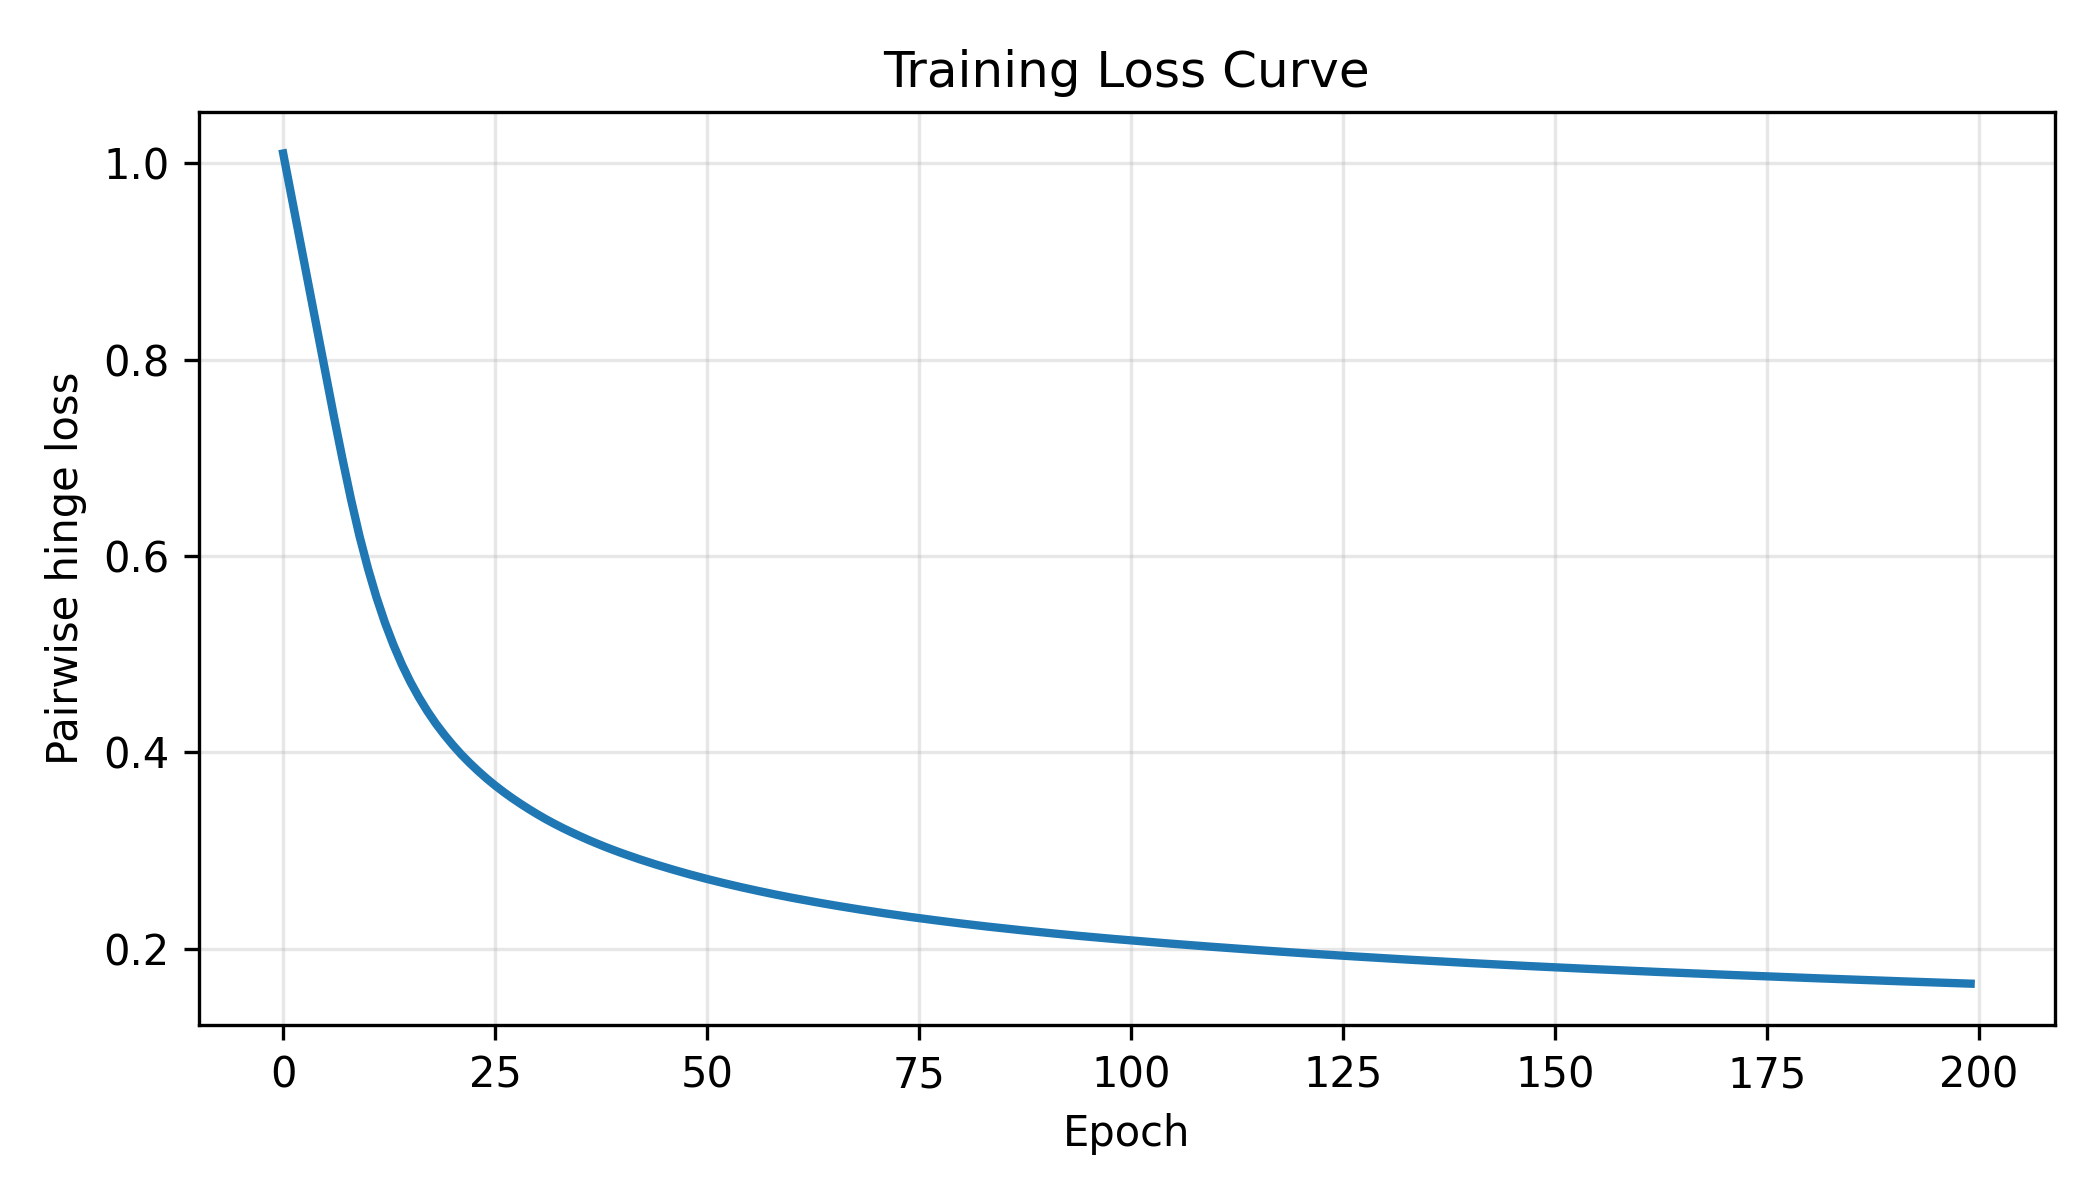
\includegraphics[width=0.85\textwidth]{figures/loss_curve.png}
    \caption{Đường cong pairwise hinge loss trong quá trình huấn luyện. Loss giảm nhanh ở các epoch đầu và tiếp tục giảm chậm dần về sau, cho thấy quá trình tối ưu đang hội tụ.}
    \label{fig:loss-curve}
\end{figure}

Loss giảm mạnh ở giai đoạn đầu và giảm chậm dần về sau. Điều này phù hợp với gradient descent: ban đầu mô hình còn sai nhiều nên gradient lớn; khi số cặp vi phạm margin giảm, tốc độ cải thiện cũng nhỏ hơn.

\subsection{So sánh ranking thật và ranking dự đoán}

Hình~\ref{fig:ranking-comparison} so sánh thứ tự ranking thật và thứ tự ranking dự đoán sau khi huấn luyện.

\begin{figure}[H]
    \centering
    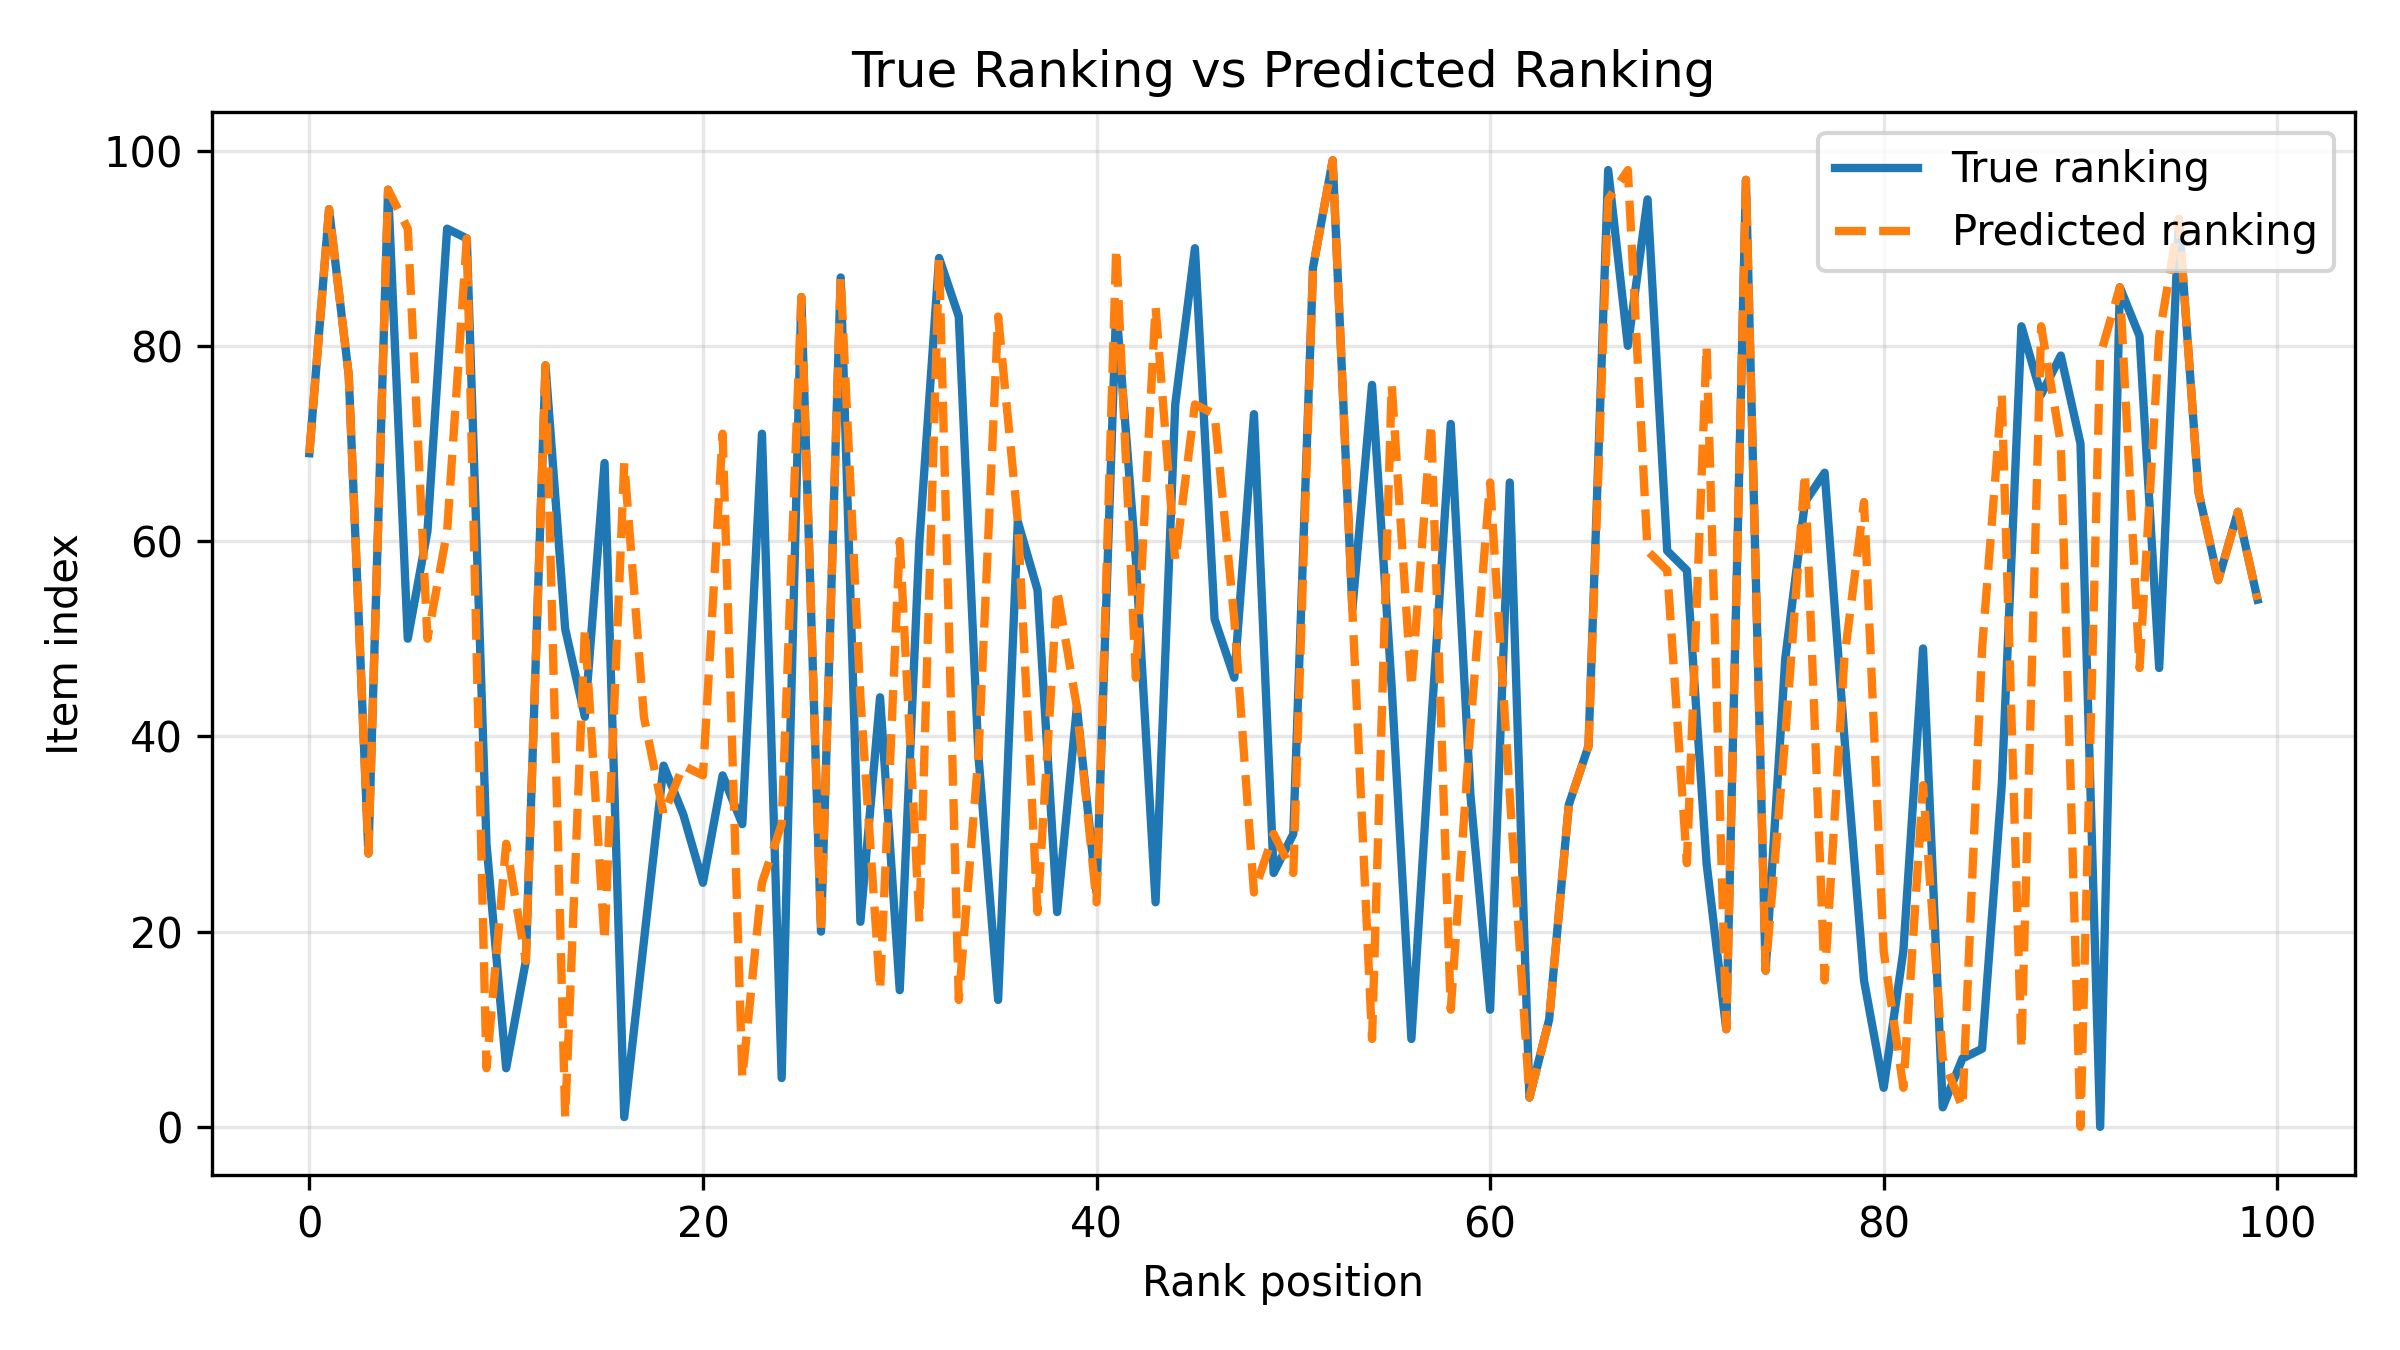
\includegraphics[width=0.9\textwidth]{figures/ranking_comparison.png}
    \caption{So sánh thứ tự ranking thật và ranking dự đoán. Hai đường càng gần nhau thì mô hình càng bảo toàn tốt quan hệ thứ tự giữa các mẫu.}
    \label{fig:ranking-comparison}
\end{figure}

Ranking dự đoán có xu hướng bám sát ranking thật. Tuy nhiên, do trục tung biểu diễn chỉ số mẫu theo từng vị trí xếp hạng, đồ thị có dạng dao động mạnh. Vì vậy, kết luận định lượng nên dựa chủ yếu vào pairwise accuracy, ranking loss và Kendall tau distance.

\subsection{Ảnh hưởng của nhiễu đến chất lượng ranking}

Để kiểm chứng ảnh hưởng của nhiễu, nhóm giữ cố định \(n=100\) và thay đổi độ lệch chuẩn nhiễu:
\[
    \sigma \in \{0.0,0.1,0.3,0.5,1.0\}.
\]

Kết quả được trình bày trong Bảng~\ref{tab:noise-results} và Hình~\ref{fig:noise-experiment}.

\begin{table}[H]
\centering
\caption{Ảnh hưởng của nhiễu đến chất lượng ranking}
\label{tab:noise-results}
\begin{tabular}{rrrrr}
\toprule
\textbf{Noise} & \textbf{Pairwise acc.} & \textbf{Ranking loss} & \textbf{Kendall tau} & \textbf{Top-10 overlap} \\
\midrule
0.0 & 0.996162 & 0.003838 & 0.003838 & 1.0 \\
0.1 & 0.985455 & 0.014545 & 0.014545 & 0.9 \\
0.3 & 0.945859 & 0.054141 & 0.054141 & 1.0 \\
0.5 & 0.914141 & 0.085859 & 0.085859 & 0.8 \\
1.0 & 0.838384 & 0.161616 & 0.161616 & 0.7 \\
\bottomrule
\end{tabular}
\end{table}

\begin{figure}[H]
    \centering
    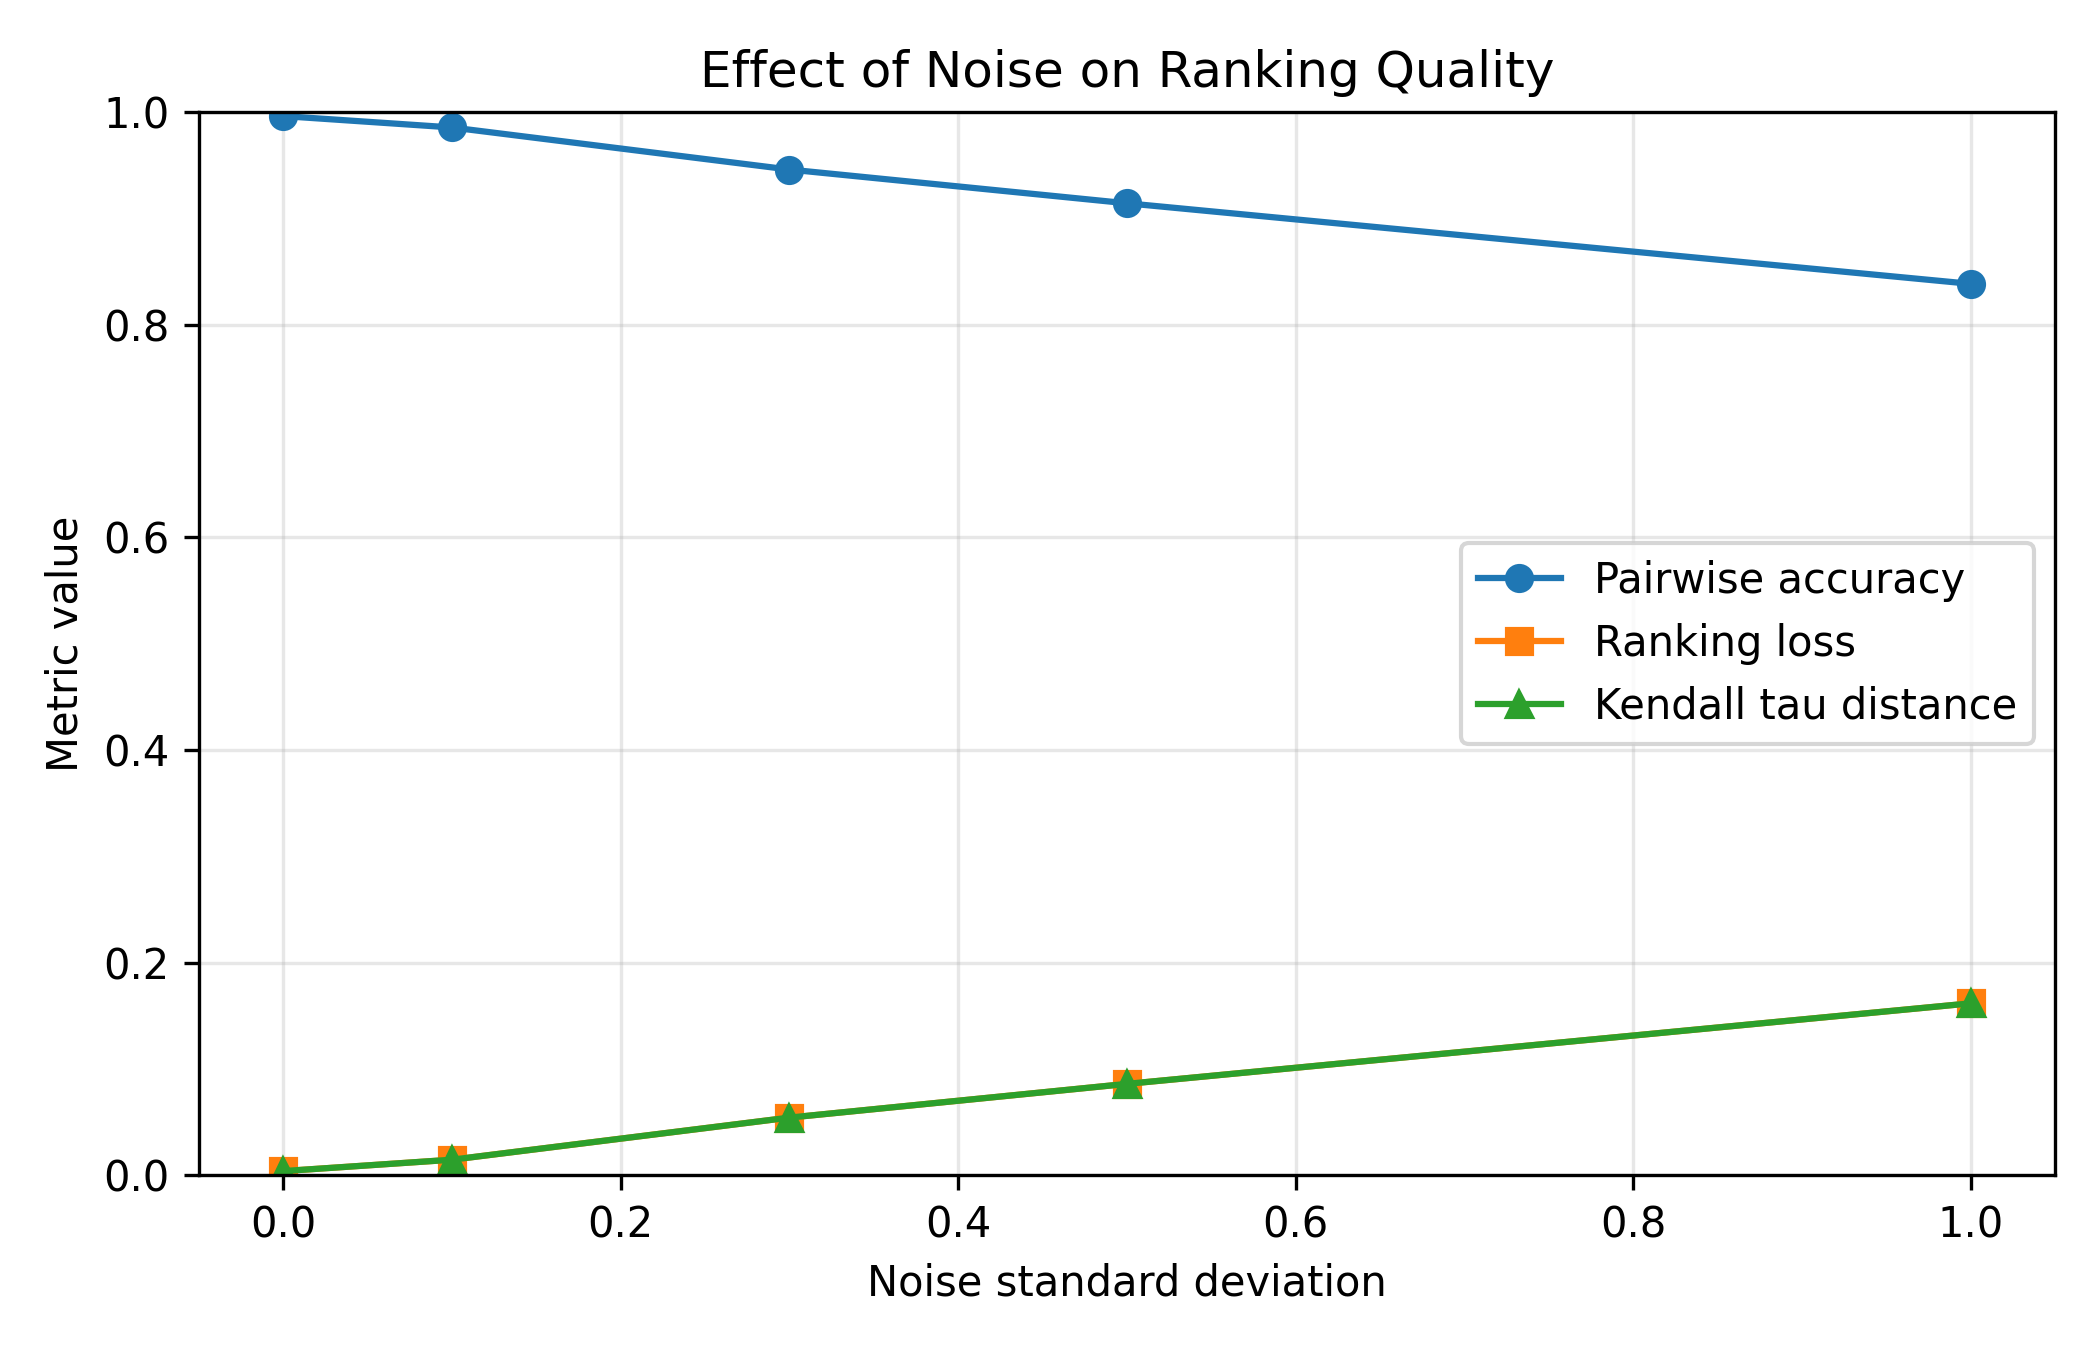
\includegraphics[width=0.9\textwidth]{figures/noise_experiment.png}
    \caption{Ảnh hưởng của độ lệch chuẩn nhiễu đến chất lượng ranking. Khi nhiễu tăng, pairwise accuracy giảm, trong khi ranking loss và Kendall tau distance tăng.}
    \label{fig:noise-experiment}
\end{figure}

Khi nhiễu tăng, chất lượng ranking giảm rõ rệt. Với \(\sigma=0.0\), dữ liệu gần như hoàn toàn tuyến tính nên pairwise accuracy đạt khoảng \(0.996\). Khi \(\sigma=1.0\), pairwise accuracy giảm xuống khoảng \(0.838\), ranking loss tăng lên khoảng \(0.162\), và top-10 overlap giảm còn \(0.7\). Điều này cho thấy nhiễu làm quan hệ ưu tiên kém ổn định hơn, khiến mô hình khó khôi phục ranking đúng.

\subsection{Ảnh hưởng của kích thước mẫu}

Trong thí nghiệm tiếp theo, nhóm cố định \(\sigma=0.1\) và thay đổi số lượng mẫu:
\[
    n \in \{20,50,100,200,500\}.
\]

Kết quả được trình bày trong Bảng~\ref{tab:sample-size-results} và Hình~\ref{fig:sample-size-experiment}.

\begin{table}[H]
\centering
\caption{Ảnh hưởng của kích thước mẫu đến chất lượng ranking}
\label{tab:sample-size-results}
\begin{tabular}{rrrrr}
\toprule
\textbf{Số mẫu} & \textbf{Pairwise acc.} & \textbf{Ranking loss} & \textbf{Kendall tau} & \textbf{Top-10 overlap} \\
\midrule
20  & 0.957895 & 0.042105 & 0.042105 & 0.9 \\
50  & 0.969796 & 0.030204 & 0.030204 & 0.9 \\
100 & 0.985455 & 0.014545 & 0.014545 & 0.9 \\
200 & 0.985829 & 0.014171 & 0.014171 & 0.9 \\
500 & 0.984858 & 0.015142 & 0.015142 & 1.0 \\
\bottomrule
\end{tabular}
\end{table}

\begin{figure}[H]
    \centering
    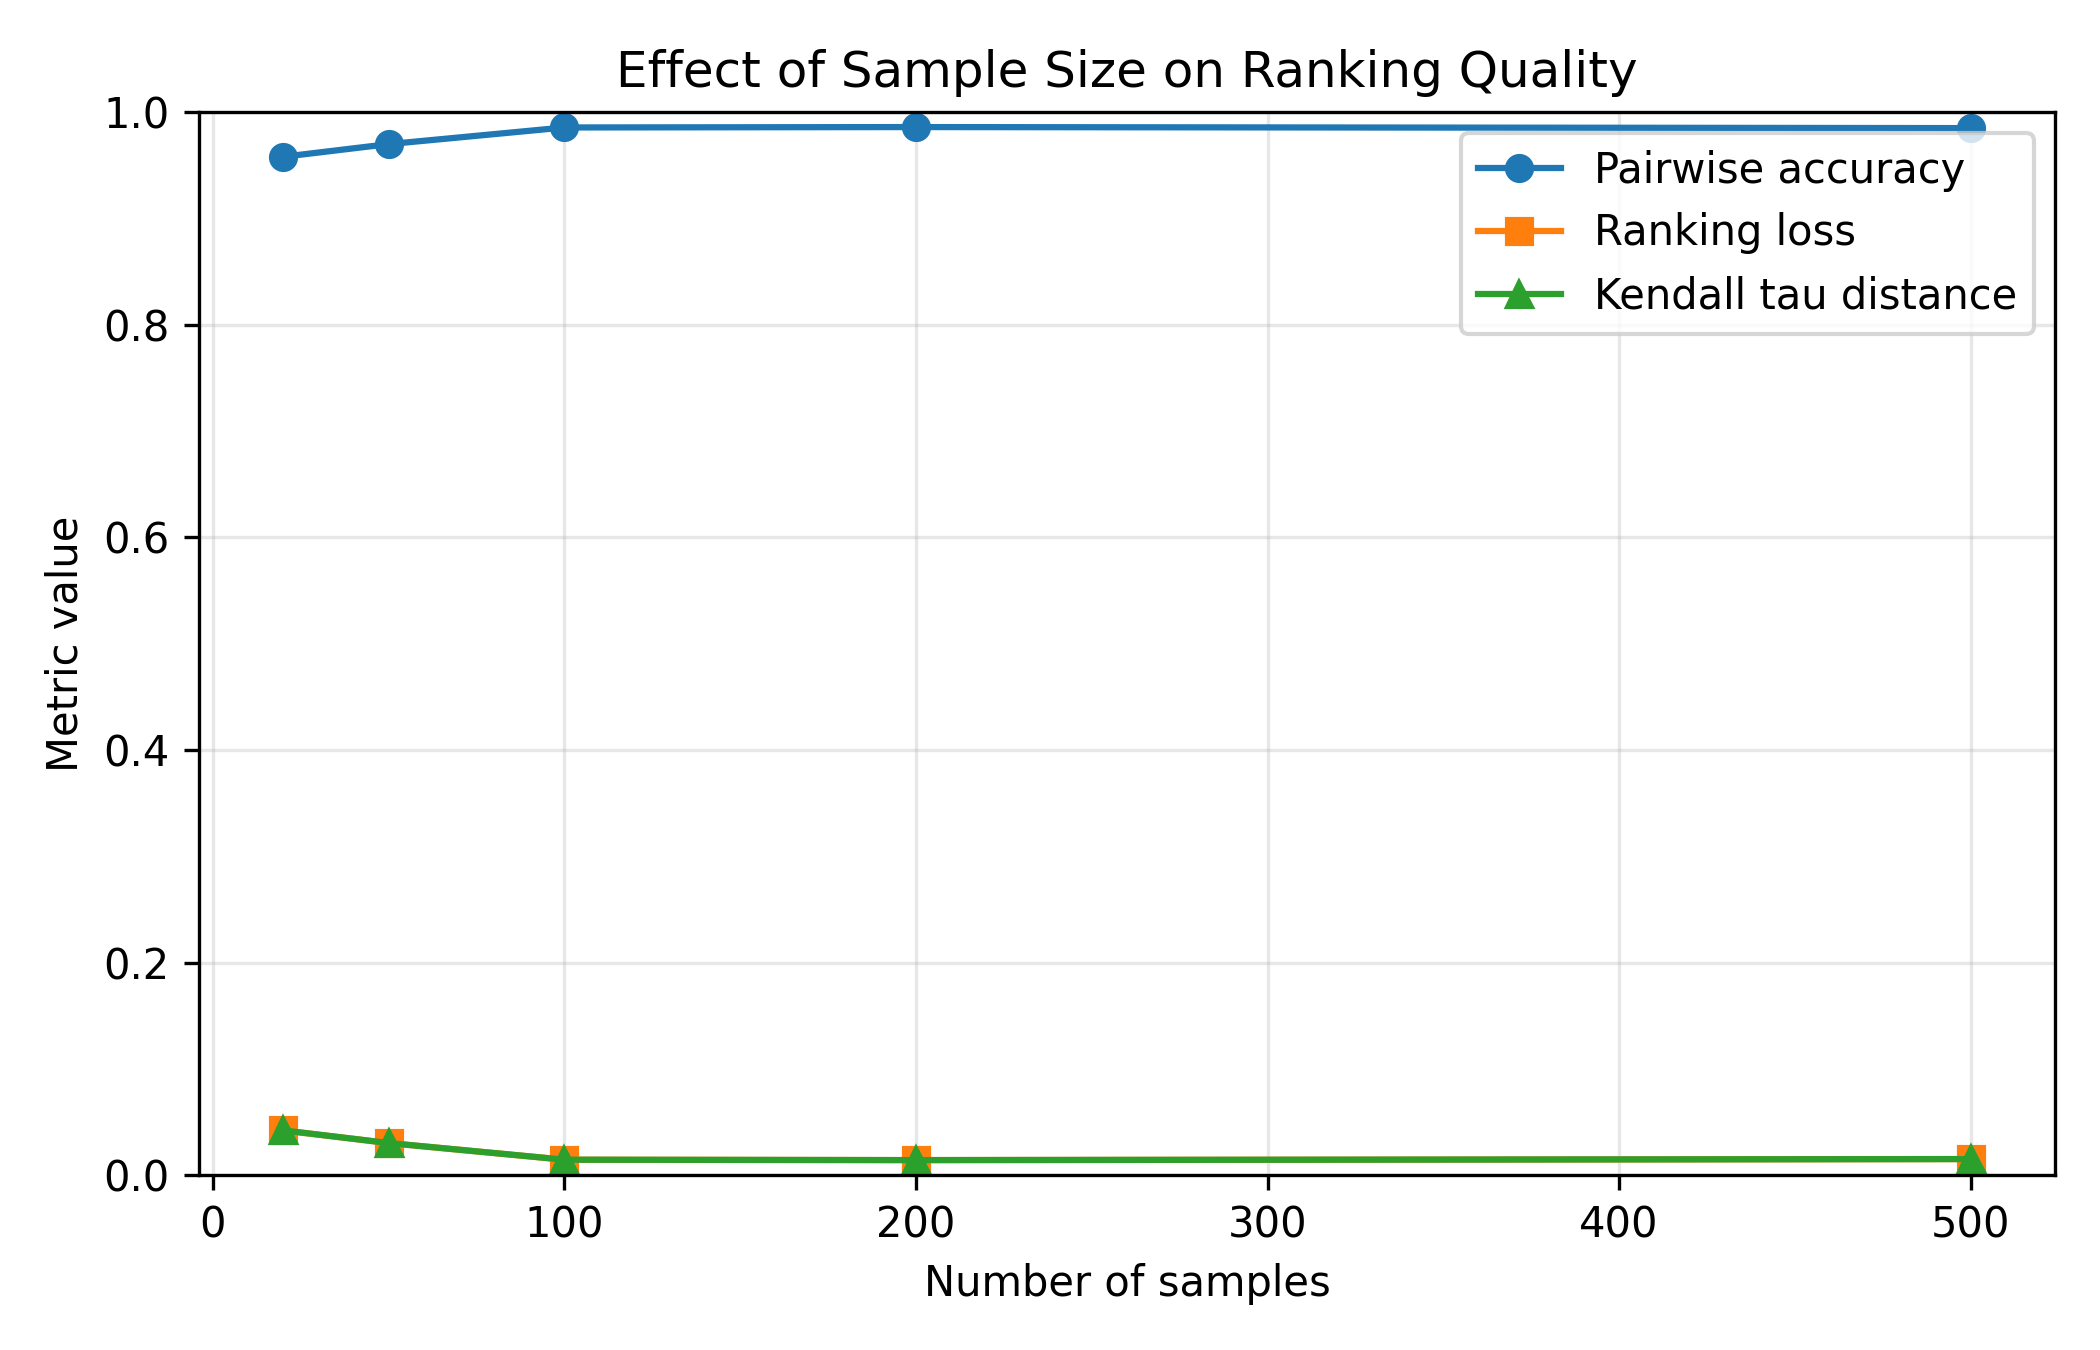
\includegraphics[width=0.9\textwidth]{figures/sample_size_experiment.png}
    \caption{Ảnh hưởng của kích thước mẫu đến chất lượng ranking. Khi số mẫu tăng, pairwise accuracy nhìn chung tăng và ranking loss giảm, sau đó ổn định ở mức tốt.}
    \label{fig:sample-size-experiment}
\end{figure}

Khi số mẫu tăng từ \(20\) lên \(100\), pairwise accuracy tăng và ranking loss giảm. Khi số mẫu tiếp tục tăng lên \(200\) và \(500\), chất lượng ranking duy trì ở mức cao. Do dữ liệu được sinh từ mô hình tuyến tính đơn giản và nhiễu nhỏ, mô hình đã đạt kết quả tốt ngay cả khi số mẫu chưa quá lớn.

\subsection{Khả năng tái tạo thực nghiệm}

Các thực nghiệm được thiết kế để có thể tái tạo. Nhóm sử dụng random seed cố định trong quá trình sinh dữ liệu, khởi tạo mô hình và chạy thực nghiệm. Các tham số như số mẫu, số đặc trưng, số epoch, learning rate và regularization đều được ghi rõ.

Các kết quả được lưu thành các file CSV:
\begin{itemize}
    \item \texttt{results/tables/main\_results.csv}: kết quả thực nghiệm chính.
    \item \texttt{results/tables/noise\_results.csv}: kết quả thí nghiệm thay đổi mức nhiễu.
    \item \texttt{results/tables/sample\_size\_results.csv}: kết quả thí nghiệm thay đổi kích thước mẫu.
\end{itemize}

Các hình minh hoạ được lưu trong thư mục \texttt{figures/}. Các thư viện chính gồm \texttt{numpy}, \texttt{matplotlib}, \texttt{csv} và \texttt{pathlib}. Phiên bản cụ thể của các thư viện được liệt kê trong file \texttt{requirements.txt}.

\subsection{Nhận xét chung}

Các thực nghiệm cho thấy mô hình pairwise ranking tuyến tính có thể học tốt quan hệ ưu tiên khi dữ liệu được sinh từ một hàm tuyến tính. Điều này thể hiện qua pairwise accuracy cao, ranking loss thấp và top-10 overlap tốt.

Đường cong loss cho thấy quá trình huấn luyện có xu hướng hội tụ. Khi nhiễu tăng, số lượng cặp bị đảo thứ tự tăng lên, làm giảm pairwise accuracy và tăng ranking loss. Khi kích thước mẫu tăng, mô hình quan sát được nhiều cặp ưu tiên hơn nên học ổn định hơn, dù mức cải thiện sau \(100\) mẫu không còn quá lớn.

Nhìn chung, kết quả thực nghiệm phù hợp với lý thuyết về pairwise learning-to-rank: mô hình học một hàm scoring sao cho bảo toàn nhiều nhất có thể các quan hệ ưu tiên giữa các cặp mẫu.

\section{Tổng hợp và thảo luận các bài báo liên quan}

Sau khi trình bày các khái niệm nền tảng của learning-to-rank, phần này tổng hợp một số bài báo liên quan nhằm làm rõ cách các lý thuyết trong chương được sử dụng và mở rộng trong các nghiên cứu hiện đại. Các bài báo được chọn đại diện cho ba hướng phát triển khác nhau: tối ưu metric ranking trong các mô hình boosting, diễn giải decision-focused learning như một bài toán ranking, và phân tích lý thuyết cho label ranking trong điều kiện có nhiễu.

Với mỗi bài báo, ta trình bày ba nội dung chính: bài toán đặt ra, đóng góp chính và mối liên hệ với các lý thuyết đã trình bày trong chương. Cuối phần là nhận xét tổng quan về xu hướng phát triển của lĩnh vực, các hạn chế còn tồn tại và một số câu hỏi mở.

\subsection{Bài báo 1: Which Tricks are Important for Learning to Rank?}

Bài báo \textit{Which Tricks are Important for Learning to Rank?} nghiên cứu các thuật toán learning-to-rank dựa trên gradient-boosted decision trees, trong đó có LambdaMART, YetiRank, StochasticRank và biến thể mới YetiLoss. Bối cảnh của bài báo là các hệ thống learning-to-rank thực tế, đặc biệt trong truy xuất thông tin, nơi mô hình cần xếp hạng danh sách tài liệu theo mức độ liên quan với truy vấn.

\subsubsection{Bài toán đặt ra}

Bài toán chính của bài báo là tìm hiểu những yếu tố kỹ thuật nào thực sự quan trọng khi huấn luyện mô hình learning-to-rank. Cụ thể, bài báo đặt ra các câu hỏi:

\begin{itemize}
    \item Có nên tối ưu trực tiếp một ranking loss đã được làm trơn hay nên tối ưu một surrogate loss lồi?
    \item Việc làm trơn ranking loss bằng nhiễu ngẫu nhiên có giúp cải thiện chất lượng mô hình không?
    \item Các cách xây dựng upper bound khác nhau ảnh hưởng như thế nào đến hiệu quả của thuật toán?
    \item Liệu có thể mở rộng YetiRank để tối ưu các metric cụ thể như MRR, MAP, ERR hay NDCG không?
\end{itemize}

Đây là bài toán quan trọng vì ranking loss thường phụ thuộc vào phép sắp xếp, mà phép sắp xếp là không khả vi. Do đó, các thuật toán học như gradient boosting không thể tối ưu trực tiếp ranking metric nếu không có một dạng surrogate hoặc một cách làm trơn phù hợp.

\subsubsection{Đóng góp chính}

Đóng góp đầu tiên của bài báo là phân tích các thuật toán GBDT-based learning-to-rank trong cùng một thiết lập thực nghiệm. Thay vì chỉ so sánh kết quả cuối cùng, bài báo phân tích vai trò của từng thành phần như smoothing, convex upper bound và cách chọn các cặp tài liệu dùng trong gradient.

Đóng góp thứ hai là chỉ ra rằng YetiRank ngầm tối ưu một dạng biến thể của DCG với discount hàm mũ. Từ quan sát này, bài báo đề xuất YetiLoss, một biến thể của YetiRank cho phép thay đổi trọng số gradient theo ranking metric mong muốn. Nhờ đó, YetiLoss có thể tối ưu các metric như MRR, MAP hoặc ERR thay vì chỉ phù hợp với một dạng DCG cố định.

Đóng góp thứ ba là kết quả thực nghiệm trên nhiều bộ dữ liệu learning-to-rank chuẩn. Bài báo cho thấy YetiRank đạt kết quả rất tốt với NDCG, trong khi YetiLoss thường tốt hơn với MAP và MRR. Ngoài ra, bài báo cũng chỉ ra rằng smoothing có vai trò quan trọng: khi bỏ smoothing, chất lượng của YetiLoss giảm rõ rệt.

\subsubsection{Liên hệ với lý thuyết trong chương}

Bài báo này liên hệ trực tiếp với phần score-based ranking. Mô hình học một hàm điểm \(f(x)\), sau đó sắp xếp các tài liệu theo điểm số để tạo ranking. Đây chính là thiết lập:
\[
    x \mapsto f(x),
\]
trong đó ranking được sinh ra bằng cách sắp xếp các giá trị \(f(x)\).

Bài báo cũng liên hệ với phần ranking loss và các tiêu chí đánh giá như NDCG, MAP, MRR và ERR. Trong chương, ta đã thấy các metric này không chỉ đo cặp đúng sai như pairwise loss, mà còn nhấn mạnh vị trí của tài liệu trong danh sách. Bài báo mở rộng ý tưởng này bằng cách nghiên cứu cách tối ưu trực tiếp hoặc gián tiếp các metric đó trong mô hình GBDT.

Ngoài ra, bài báo còn liên hệ với phần surrogate loss. Vì ranking loss không khả vi, các thuật toán như LambdaMART xây dựng upper bound khả vi để tối ưu. YetiLoss cũng dùng surrogate nhưng khác LambdaMART ở chỗ nó chỉ xét các hoán vị lân cận trong ranking sau khi thêm nhiễu. Điều này gần với trực giác rằng một bước cập nhật nhỏ của mô hình chỉ có thể làm thay đổi cục bộ thứ tự ranking.

\subsubsection{Hạn chế và nhận xét}

Một hạn chế của bài báo là phạm vi phân tích chủ yếu tập trung vào mô hình GBDT. Đây là lựa chọn hợp lý vì GBDT vẫn rất mạnh trên dữ liệu bảng, nhưng kết luận của bài báo chưa chắc chuyển trực tiếp sang các mô hình neural ranking. Ngoài ra, YetiLoss cho kết quả tốt với MAP và MRR, nhưng với NDCG thì YetiRank vẫn thường mạnh hơn. Điều này cho thấy không có một thuật toán duy nhất tối ưu cho mọi metric.

Một hướng mở tự nhiên là nghiên cứu liệu các kết luận về smoothing, local permutation và convex surrogate có còn đúng trong neural rankers, recommender systems hoặc các bài toán ranking có dữ liệu đa phương thức hay không.

\subsection{Bài báo 2: Decision-Focused Learning: Through the Lens of Learning to Rank}

Bài báo \textit{Decision-Focused Learning: Through the Lens of Learning to Rank} mở rộng learning-to-rank sang một bối cảnh khác: decision-focused learning, hay còn gọi là predict-and-optimize. Trong thiết lập này, mô hình học máy không chỉ dự đoán một đại lượng trung gian, mà dự đoán các tham số được đưa vào một bài toán tối ưu tổ hợp ở bước sau.

\subsubsection{Bài toán đặt ra}

Trong predict-and-optimize, ta thường có một bài toán tối ưu tổ hợp với hàm mục tiêu phụ thuộc vào một vector tham số chưa biết \(c\). Mô hình học máy nhận đầu vào \(x\) và dự đoán \(\hat{c}\). Sau đó, lời giải tối ưu được tính bằng cách giải bài toán tối ưu với \(\hat{c}\). Mục tiêu cuối cùng không phải là dự đoán \(\hat{c}\) thật gần \(c\), mà là tạo ra quyết định có regret nhỏ.

Bài toán có thể viết ở dạng:
\begin{equation}
    v^\star(c)
    \in
    \arg\min_{v\in V}
    f(v,c),
    \label{eq:section10-dfl-optimization}
\end{equation}
trong đó \(V\) là tập nghiệm khả thi của bài toán tối ưu tổ hợp. Regret của dự đoán \(\hat{c}\) được định nghĩa là:
\begin{equation}
    \mathrm{Regret}(\hat{c},c)
    =
    f(v^\star(\hat{c}),c)
    -
    f(v^\star(c),c).
    \label{eq:section10-dfl-regret}
\end{equation}

Khó khăn chính là ánh xạ \(\hat{c}\mapsto v^\star(\hat{c})\) thường không khả vi vì \(V\) là tập rời rạc. Do đó, việc lan truyền gradient qua bộ giải tối ưu tổ hợp là rất khó và tốn kém.

\subsubsection{Đóng góp chính}

Đóng góp quan trọng nhất của bài báo là diễn giải decision-focused learning như một bài toán learning-to-rank. Với mỗi instance, các nghiệm khả thi \(v\in V\) được xem như các ``items'' cần xếp hạng. Hàm mục tiêu \(f(v,c)\) tạo ra thứ tự đúng trên các nghiệm khả thi: nghiệm có giá trị mục tiêu nhỏ hơn nên được xếp cao hơn.

Từ góc nhìn này, thay vì cố gắng đạo hàm trực tiếp qua nghiệm tối ưu \(v^\star(\hat{c})\), bài báo đề xuất học sao cho hàm mục tiêu dự đoán \(f(v,\hat{c})\) tạo ra cùng thứ tự với hàm mục tiêu thật \(f(v,c)\) trên một tập con nghiệm khả thi \(S\subseteq V\). Vì không thể liệt kê toàn bộ \(V\), bài báo dùng một tập nghiệm con \(S\) và cập nhật dần trong quá trình huấn luyện.

Bài báo đề xuất ba nhóm loss theo learning-to-rank:

\begin{itemize}
    \item \textit{Pointwise loss}: so khớp giá trị mục tiêu dự đoán và giá trị mục tiêu thật trên từng nghiệm.
    \item \textit{Pairwise loss}: yêu cầu nghiệm tốt hơn theo \(c\) cũng phải có điểm tốt hơn theo \(\hat{c}\).
    \item \textit{Listwise loss}: so sánh phân phối xác suất trên toàn bộ danh sách nghiệm trong tập \(S\).
\end{itemize}

Đặc biệt, bài báo chỉ ra rằng loss noise-contrastive estimation trong nghiên cứu trước có thể được xem như một trường hợp đặc biệt của pairwise ranking theo dạng best-versus-rest.

\subsubsection{Liên hệ với lý thuyết trong chương}

Bài báo này liên hệ rõ với cả score-based ranking và pairwise ranking. Trong chương, ta học hàm điểm \(h(x)\) để sắp xếp các đối tượng. Ở đây, đối tượng cần xếp hạng không phải là tài liệu hay sản phẩm, mà là các nghiệm khả thi \(v\) của một bài toán tối ưu. Hàm điểm tương ứng là:
\[
    v \mapsto -f(v,\hat{c}),
\]
nếu bài toán là bài toán cực tiểu. Nghiệm có giá trị mục tiêu nhỏ hơn sẽ có điểm ranking cao hơn.

Pairwise loss trong bài báo cũng rất gần với Ranking SVM và pairwise hinge loss đã trình bày. Với một cặp nghiệm \((v^p,v^q)\), nếu \(v^p\) tốt hơn \(v^q\) theo \(c\), ta muốn:
\[
    f(v^p,\hat{c}) < f(v^q,\hat{c}).
\]
Dạng margin ranking loss của bài báo có cùng tinh thần với pairwise hinge loss: không chỉ yêu cầu đúng thứ tự, mà còn muốn có một khoảng cách đủ lớn giữa nghiệm tốt và nghiệm kém hơn.

Bài báo cũng liên hệ với phần preference-based ranking. Trong decision-focused learning, ta có thể xem mỗi cặp nghiệm khả thi như một cặp ưu tiên. Nếu nghiệm \(v^p\) cho giá trị mục tiêu tốt hơn \(v^q\), thì \(v^p\succ v^q\). Do đó, học để giảm regret có thể được xem như học để bảo toàn quan hệ ưu tiên giữa các nghiệm.

\subsubsection{Hạn chế và nhận xét}

Điểm mạnh của bài báo là kết nối hai lĩnh vực tưởng như khác nhau: decision-focused learning và learning-to-rank. Tuy nhiên, phương pháp vẫn phụ thuộc vào tập nghiệm con \(S\). Nếu \(S\) không chứa các nghiệm quan trọng, loss ranking có thể không phản ánh đúng regret thật. Ngoài ra, việc mở rộng \(S\) vẫn cần gọi solver trong quá trình huấn luyện, dù số lần gọi solver có thể được kiểm soát.

Một hướng cải tiến là thiết kế chiến lược chọn nghiệm \(S\) thông minh hơn, chẳng hạn ưu tiên các nghiệm gần tối ưu, các nghiệm dễ gây nhầm lẫn hoặc các nghiệm nằm gần biên quyết định của mô hình. Điều này tương tự hard negative mining trong ranking và retrieval.

\subsection{Bài báo 3: Linear Label Ranking with Bounded Noise}

Bài báo \textit{Linear Label Ranking with Bounded Noise} nghiên cứu bài toán label ranking dưới góc nhìn lý thuyết học máy. Khác với các bài báo thực nghiệm về ranking trong truy xuất thông tin, bài báo này tập trung vào khả năng học một hàm xếp hạng tuyến tính khi dữ liệu nhãn ranking có nhiễu bị chặn.

\subsubsection{Bài toán đặt ra}

Trong label ranking, mỗi đầu vào \(x\in\mathbb{R}^d\) không chỉ có một nhãn đơn, mà có một hoán vị trên \(k\) nhãn. Một lớp mô hình tự nhiên là Linear Sorting Function, trong đó mỗi nhãn \(i\) có một vector trọng số \(W_i\), và ranking được tạo bằng cách sắp xếp các điểm:
\[
    W_1x,\; W_2x,\;\ldots,\;W_kx.
\]

Hàm mục tiêu có dạng:
\begin{equation}
    \sigma_W(x)
    =
    \operatorname{argsort}(Wx).
    \label{eq:section10-linear-sorting-function}
\end{equation}

Bài toán đặt ra là: nếu các ranking quan sát được bị nhiễu nhưng xác suất đảo sai mỗi cặp bị chặn bởi một hằng số \(\eta<1/2\), liệu ta có thể học được một hàm xếp hạng tuyến tính gần với hàm mục tiêu hay không? Độ gần được đo bằng Kendall tau distance, tức là tỉ lệ cặp nhãn bị đảo thứ tự.

\subsubsection{Đóng góp chính}

Đóng góp chính của bài báo là đưa ra thuật toán học cho Linear Sorting Functions trong điều kiện bounded noise. Ý tưởng cơ bản là chuyển bài toán ranking nhiều nhãn thành nhiều bài toán phân loại nhị phân theo cặp nhãn.

Cụ thể, với mỗi cặp nhãn \((i,j)\), ta xét xem trong ranking quan sát được nhãn nào đứng trước. Điều này tạo ra một bài toán học halfspace với nhãn nhị phân. Vì nhiễu trên ranking bị chặn, mỗi bài toán nhị phân này có thể được xem như học halfspace dưới Massart noise. Sau khi học các bộ phân loại theo từng cặp, thuật toán ghép các quan hệ cặp thành một ranking toàn cục.

Khi các quan hệ cặp tạo ra chu trình, bài báo dùng bài toán minimum feedback arc set để loại bỏ các mâu thuẫn và tạo ra một ranking hợp lệ. Kết quả lý thuyết cho thấy có thể đạt sai số nhỏ theo Kendall tau distance với số mẫu và thời gian chạy đa thức theo các tham số chính.

Bài báo cũng trình bày phiên bản proper learning, trong đó thuật toán không chỉ tạo ra một bộ phân loại cặp riêng lẻ, mà còn tìm lại một Linear Sorting Function thật sự. Điều này được thực hiện thông qua một chương trình lồi trên ma trận \(W\).

\subsubsection{Liên hệ với lý thuyết trong chương}

Bài báo này liên hệ trực tiếp với phần preference-based ranking và Kendall tau distance. Trong preference-based ranking, ta học quan hệ ưu tiên theo từng cặp rồi cần chuyển các quan hệ đó thành ranking toàn cục. Bài báo này làm đúng điều đó trong bối cảnh label ranking: mỗi cặp nhãn \((i,j)\) được học bằng một halfspace, sau đó các dự đoán cặp được ghép thành một thứ tự đầy đủ.

Bài báo cũng liên hệ với phần sort-by-degree và randomized QuickSort theo nghĩa rộng: cả ba đều xử lý bài toán chuyển quan hệ cặp thành ranking toàn cục. Tuy nhiên, bài báo này dùng công cụ lý thuyết mạnh hơn, cụ thể là đồ thị tournament và minimum feedback arc set, để xử lý trường hợp quan hệ cặp không nhất quán.

Ngoài ra, việc dùng Kendall tau distance làm thước đo sai số phù hợp với phần tiêu chí đánh giá ranking đã trình bày. Kendall tau đo tỉ lệ cặp bị đảo, nên rất tự nhiên khi phân tích các thuật toán học dựa trên cặp nhãn.

\subsubsection{Hạn chế và nhận xét}

Hạn chế chính của hướng tiếp cận này là tính lý thuyết cao và giả định tương đối mạnh. Phân tích thường dựa trên mô hình nhiễu bị chặn và phân phối đầu vào có cấu trúc tốt, chẳng hạn Gaussian hoặc log-concave. Trong dữ liệu thực tế, nhiễu có thể không đồng đều, phụ thuộc vào từng vùng dữ liệu hoặc từng cặp nhãn.

Ngoài ra, số lượng cặp nhãn là \(O(k^2)\), nên khi số nhãn \(k\) lớn, việc học tất cả các bộ phân loại cặp có thể tốn kém. Đây cũng là hạn chế chung của nhiều phương pháp pairwise ranking.

Một hướng mở là kết hợp lý thuyết bounded noise với các mô hình thực nghiệm hiện đại, chẳng hạn neural ranking hoặc gradient boosting, để vừa giữ được bảo đảm lý thuyết vừa có khả năng áp dụng trên dữ liệu lớn.

\subsection{Nhận xét tổng quan về xu hướng phát triển}

Từ ba bài báo trên, có thể thấy learning-to-rank đang phát triển theo ba xu hướng chính.

\subsubsection{Từ pairwise ranking sang tối ưu metric trực tiếp}

Các phương pháp cổ điển như Ranking SVM hay RankBoost thường tối ưu pairwise loss. Tuy nhiên, trong các ứng dụng thực tế, metric cuối cùng thường là NDCG, MAP, MRR hoặc ERR. Bài báo về YetiLoss cho thấy xu hướng hiện đại là thiết kế thuật toán sao cho gần hơn với metric thực sự được quan tâm. Thay vì chỉ đếm số cặp đúng sai, các thuật toán mới cố gắng đưa thông tin về vị trí trong danh sách và độ quan trọng của từng metric vào gradient.

\subsubsection{Sử dụng smoothing và surrogate loss để xử lý tính không khả vi}

Một vấn đề trung tâm của ranking là phép sắp xếp không khả vi. Các bài báo hiện đại xử lý vấn đề này theo hai hướng: xây dựng surrogate loss khả vi hoặc làm trơn ranking loss bằng nhiễu ngẫu nhiên. LambdaMART dùng upper bound khả vi, YetiRank và YetiLoss dùng smoothing trên thứ tự ranking, còn StochasticRank tối ưu loss được làm trơn trực tiếp. Điều này cho thấy smoothing và surrogate loss là hai công cụ quan trọng để kết nối ranking metric rời rạc với các thuật toán tối ưu gradient.

\subsubsection{Mở rộng learning-to-rank ra ngoài truy xuất thông tin}

Bài báo về decision-focused learning cho thấy learning-to-rank không chỉ dùng cho tìm kiếm tài liệu hay hệ gợi ý. Khi các nghiệm khả thi của một bài toán tối ưu tổ hợp được xem như các items cần xếp hạng, ta có thể dùng ranking loss để huấn luyện mô hình dự đoán tham số. Đây là một hướng mở rộng quan trọng, vì nó biến learning-to-rank thành một công cụ chung cho các bài toán ra quyết định.

\subsubsection{Tăng cường phân tích lý thuyết cho ranking có nhiễu}

Bài báo về Linear Label Ranking with Bounded Noise cho thấy một hướng khác: xây dựng bảo đảm học được trong môi trường có nhiễu. Thay vì chỉ đánh giá thực nghiệm, bài báo phân tích số mẫu, độ phức tạp thuật toán và sai số theo Kendall tau distance. Điều này bổ sung nền tảng lý thuyết cho các phương pháp pairwise và preference-based ranking.

\subsection{Hạn chế chung của các phương pháp}

Dù các hướng tiếp cận trên có nhiều đóng góp, vẫn còn một số hạn chế chung.

Thứ nhất, nhiều phương pháp ranking vẫn phụ thuộc mạnh vào surrogate loss. Surrogate loss giúp tối ưu dễ hơn, nhưng không phải lúc nào cũng khớp hoàn toàn với metric cuối cùng. Ví dụ, tối ưu pairwise loss có thể không tối ưu tốt NDCG@10 nếu các lỗi ở đầu danh sách quan trọng hơn nhiều so với lỗi ở cuối danh sách.

Thứ hai, các phương pháp pairwise thường có chi phí lớn vì số cặp tăng theo \(O(n^2)\) hoặc \(O(k^2)\). Điều này xuất hiện trong Ranking SVM, RankBoost, preference-based ranking và cả label ranking theo cặp nhãn. Khi số đối tượng hoặc số nhãn lớn, cần có chiến lược lấy mẫu cặp hoặc chọn cặp quan trọng.

Thứ ba, nhiều kết quả lý thuyết cần giả định khá mạnh, chẳng hạn nhiễu bị chặn, phân phối đầu vào chuẩn hoặc log-concave. Những giả định này giúp phân tích rõ ràng, nhưng có thể không phản ánh đầy đủ dữ liệu thực tế.

Thứ tư, trong các hệ thống thực tế, ranking thường chịu ảnh hưởng của nhiều yếu tố khác như fairness, robustness, distribution shift, cold-start và feedback loop. Các yếu tố này chưa được xử lý đầy đủ trong các mô hình lý thuyết cơ bản.

\subsection{Câu hỏi mở và ý tưởng cải tiến}

Một số câu hỏi mở tự nhiên từ các bài báo trên là:

\begin{itemize}
    \item Làm thế nào để tối ưu trực tiếp các metric như NDCG, MAP hoặc MRR mà vẫn có bảo đảm hội tụ và tổng quát hoá?
    \item Có thể thiết kế surrogate loss vừa khả vi, vừa bám sát metric cuối cùng hơn pairwise hinge loss hay không?
    \item Trong preference-based ranking, làm thế nào để xử lý quan hệ ưu tiên không bắc cầu một cách hiệu quả khi số đối tượng rất lớn?
    \item Với decision-focused learning, nên chọn tập nghiệm con \(S\) như thế nào để vừa giảm chi phí gọi solver, vừa giữ được thông tin quan trọng cho regret?
    \item Các bảo đảm lý thuyết trong label ranking có thể mở rộng sang neural networks hoặc dữ liệu không Gaussian hay không?
\end{itemize}

Từ các câu hỏi trên, có thể đề xuất một số ý tưởng cải tiến. Với các thuật toán pairwise, có thể dùng hard pair mining, tức là chỉ chọn các cặp mà mô hình đang dễ nhầm hoặc các cặp ảnh hưởng lớn đến metric top-\(k\). Với decision-focused learning, có thể cập nhật tập nghiệm \(S\) bằng cách kết hợp nghiệm tối ưu thật, nghiệm dự đoán hiện tại và các nghiệm gần tối ưu. Với các thuật toán như YetiLoss, có thể thử nghiệm các phân phối smoothing khác nhau hoặc học tham số smoothing thay vì cố định trước.

\subsection{Kết luận}

Ba bài báo được trình bày cho thấy learning-to-rank là một lĩnh vực có cả chiều sâu lý thuyết lẫn giá trị thực tiễn. Bài báo về YetiLoss tập trung vào tối ưu metric ranking trong các mô hình GBDT hiện đại. Bài báo về decision-focused learning cho thấy ranking có thể được dùng để huấn luyện mô hình ra quyết định trong tối ưu tổ hợp. Bài báo về Linear Label Ranking with Bounded Noise cung cấp góc nhìn lý thuyết về khả năng học ranking khi dữ liệu có nhiễu.

Nhìn chung, các bài báo đều nhấn mạnh cùng một ý tưởng cốt lõi: chất lượng của mô hình ranking không chỉ nằm ở việc dự đoán đúng từng điểm riêng lẻ, mà nằm ở việc bảo toàn đúng quan hệ thứ tự giữa các đối tượng. Đây cũng chính là tinh thần xuyên suốt của chương về learning-to-rank.
\section{Kết luận}

Chương này đã trình bày tổng quan về bài toán \textit{learning-to-rank}, từ các khái niệm nền tảng đến một số thuật toán, tiêu chí đánh giá, thực nghiệm minh hoạ và các hướng nghiên cứu liên quan. Khác với bài toán phân loại hoặc hồi quy thông thường, ranking không chỉ quan tâm đến dự đoán trên từng đối tượng riêng lẻ, mà tập trung vào quan hệ thứ tự giữa các đối tượng. Đây là điểm làm cho ranking trở thành một bài toán quan trọng trong nhiều ứng dụng như truy xuất thông tin, công cụ tìm kiếm, hệ gợi ý, phát hiện gian lận và ra quyết định tối ưu.

Trước hết, chương đã giới thiệu các thiết lập cơ bản của ranking, bao gồm \textit{score-based ranking} và \textit{preference-based ranking}. Trong score-based ranking, mô hình học một hàm điểm
\[
    h:\mathcal{X}\rightarrow\mathbb{R},
\]
sau đó sinh ranking bằng cách sắp xếp các đối tượng theo điểm số. Trong preference-based ranking, mô hình học trực tiếp quan hệ ưu tiên giữa từng cặp đối tượng. Hai thiết lập này cho thấy ranking có thể được tiếp cận theo nhiều cách khác nhau, tuỳ thuộc vào dạng dữ liệu huấn luyện và mục tiêu ứng dụng.

Tiếp theo, chương đã trình bày các khái niệm lý thuyết quan trọng như lỗi xếp hạng theo từng cặp, margin, pairwise loss và chặn tổng quát hoá dựa trên Rademacher complexity. Các kết quả này cho thấy để một mô hình ranking có khả năng tổng quát hoá tốt, ta cần đồng thời kiểm soát lỗi thực nghiệm và độ phức tạp của lớp giả thuyết. Đây là cơ sở lý thuyết cho các phương pháp ranking dựa trên margin.

Dựa trên các ý tưởng đó, chương đã trình bày hai thuật toán tiêu biểu là \textit{Ranking SVM} và \textit{RankBoost}. Ranking SVM chuyển bài toán ranking theo từng cặp thành một bài toán phân loại nhị phân trên các vector hiệu, từ đó tận dụng được nguyên lý margin của SVM. RankBoost sử dụng tư tưởng boosting, duy trì trọng số trên các cặp đối tượng và tập trung dần vào các cặp khó. Hai thuật toán này minh hoạ rõ cách các bài toán ranking có thể được giải quyết bằng cách chuyển về các bài toán học máy quen thuộc hơn.

Chương cũng đã xét trường hợp đặc biệt \textit{bipartite ranking}, trong đó mục tiêu là xếp các điểm positive cao hơn các điểm negative. Trong thiết lập này, AUC là một độ đo tự nhiên vì nó có thể được hiểu là xác suất một điểm positive được xếp cao hơn một điểm negative. Khi bỏ qua trường hợp hoà điểm, ta có quan hệ quan trọng:
\[
    \mathrm{AUC}(h)=1-R(h),
\]
trong đó \(R(h)\) là ranking loss trong bipartite ranking. Quan hệ này cho thấy AUC không chỉ là một metric thực nghiệm, mà còn có diễn giải trực tiếp dưới góc nhìn pairwise ranking.

Bên cạnh đó, chương đã thảo luận nhiều tiêu chí đánh giá ranking như pairwise accuracy, ranking loss, Kendall tau distance, AUC, Precision@\(k\), MAP, MRR và NDCG. Mỗi tiêu chí phản ánh một khía cạnh khác nhau của chất lượng ranking. Các tiêu chí pairwise phù hợp với phân tích lý thuyết và các mô hình học theo cặp, trong khi các tiêu chí như NDCG, MAP và MRR phù hợp hơn với các hệ thống truy xuất thông tin thực tế, nơi các vị trí đầu danh sách có vai trò đặc biệt quan trọng.

Phần thực nghiệm đã minh hoạ một mô hình pairwise ranking tuyến tính được cài đặt từ đầu bằng Python và NumPy. Kết quả cho thấy mô hình có thể học tốt quan hệ ưu tiên khi dữ liệu được sinh từ một hàm tuyến tính và mức nhiễu không quá lớn. Thí nghiệm cũng cho thấy khi nhiễu tăng, chất lượng ranking giảm rõ rệt; trong khi khi kích thước mẫu tăng, mô hình có xu hướng học ổn định hơn. Các kết quả này phù hợp với lý thuyết: ranking tốt đòi hỏi mô hình bảo toàn được càng nhiều quan hệ ưu tiên theo cặp càng tốt.

Cuối cùng, chương đã tổng hợp một số bài báo liên quan để cho thấy learning-to-rank vẫn là một hướng nghiên cứu đang phát triển mạnh. Các nghiên cứu hiện đại không chỉ dừng lại ở pairwise loss cổ điển, mà còn hướng đến tối ưu trực tiếp các metric như NDCG, MAP, MRR, mở rộng ranking sang decision-focused learning, và xây dựng bảo đảm lý thuyết cho label ranking trong điều kiện có nhiễu. Điều này cho thấy learning-to-rank vừa có nền tảng lý thuyết phong phú, vừa có nhiều ứng dụng thực tiễn.

Tóm lại, learning-to-rank là một bài toán trung tâm trong học máy hiện đại, đặc biệt khi mục tiêu không chỉ là dự đoán đúng từng điểm dữ liệu mà là tạo ra một thứ tự có ý nghĩa. Các mô hình và lý thuyết trong chương cho thấy bản chất của ranking nằm ở việc học và bảo toàn quan hệ ưu tiên giữa các đối tượng. Đây cũng là nền tảng để phát triển các hệ thống ranking hiệu quả hơn trong thực tế, đặc biệt trong những ứng dụng mà chất lượng của các vị trí đầu danh sách có ảnh hưởng trực tiếp đến trải nghiệm người dùng và giá trị của hệ thống.

% ================== APPENDIX ==================
\newpage
\appendix
\section{Phụ lục: Cấu trúc mã nguồn và hướng dẫn tái tạo thực nghiệm}

Phụ lục này trình bày cấu trúc thư mục mã nguồn, vai trò của từng thành phần và hướng dẫn chạy lại các thực nghiệm trong báo cáo. Toàn bộ phần thực nghiệm được tổ chức trong thư mục \texttt{code/}.

\subsection{Cấu trúc thư mục}

Cấu trúc thư mục chính của project như sau:

\begin{lstlisting}
code/
|-- experiments/
|-- results/
|-- src/
|-- tests/
|-- README.md
|-- requirements.txt
|-- run_experiments.py
|-- run_main.py
\end{lstlisting}

Trong đó:

\begin{itemize}
    \item \texttt{experiments/}: chứa các script hoặc cấu hình phục vụ cho các thí nghiệm, chẳng hạn thí nghiệm chính, thí nghiệm thay đổi mức nhiễu và thí nghiệm thay đổi kích thước mẫu.
    
    \item \texttt{results/}: lưu kết quả đầu ra của quá trình thực nghiệm, bao gồm các bảng kết quả, file CSV và hình minh hoạ được sử dụng trong báo cáo.
    
    \item \texttt{src/}: chứa mã nguồn chính của chương trình, chẳng hạn các hàm sinh dữ liệu, mô hình ranking tuyến tính, hàm mất mát, hàm huấn luyện và các độ đo đánh giá.
    
    \item \texttt{tests/}: chứa các kiểm thử đơn giản nhằm đảm bảo các thành phần quan trọng như sinh cặp ưu tiên, tính loss và tính metric hoạt động đúng.
    
    \item \texttt{README.md}: mô tả ngắn gọn project, cách cài đặt môi trường và cách chạy chương trình.
    
    \item \texttt{requirements.txt}: liệt kê các thư viện Python cần thiết để chạy lại thực nghiệm.
    
    \item \texttt{run\_main.py}: script chạy thực nghiệm chính với thiết lập mặc định.
    
    \item \texttt{run\_experiments.py}: script chạy toàn bộ các thực nghiệm, bao gồm thí nghiệm chính, thí nghiệm theo mức nhiễu và thí nghiệm theo kích thước mẫu.
\end{itemize}

\subsection{Môi trường thực nghiệm}

Các thực nghiệm được cài đặt bằng Python. Các thư viện chính được sử dụng gồm:

\begin{itemize}
    \item \texttt{numpy}: dùng cho các phép toán vector, ma trận, sinh dữ liệu và cập nhật trọng số.
    \item \texttt{matplotlib}: dùng để vẽ các hình minh hoạ như đường cong loss, so sánh ranking và các biểu đồ thí nghiệm.
    \item \texttt{csv}: dùng để lưu kết quả thực nghiệm dưới dạng bảng.
    \item \texttt{pathlib}: dùng để quản lý đường dẫn thư mục và file.
\end{itemize}

Để cài đặt các thư viện cần thiết, chạy lệnh:

\begin{lstlisting}[language=bash]
pip install -r requirements.txt
\end{lstlisting}

\subsection{Cách chạy thực nghiệm chính}

Để chạy thực nghiệm chính với cấu hình mặc định, sử dụng lệnh:

\begin{lstlisting}[language=bash]
python run_main.py
\end{lstlisting}

Script này thực hiện các bước sau:

\begin{enumerate}[label=\textbf{Bước \arabic*.}, leftmargin=*]
    \item Sinh dữ liệu tổng hợp theo mô hình tuyến tính.
    \item Sinh các cặp ưu tiên từ điểm xếp hạng thật.
    \item Khởi tạo mô hình scoring tuyến tính.
    \item Huấn luyện mô hình bằng pairwise hinge loss.
    \item Tính các metric đánh giá như pairwise accuracy, ranking loss, Kendall tau distance và top-\(k\) overlap.
    \item Lưu kết quả và hình minh hoạ vào thư mục \texttt{results/}.
\end{enumerate}

\subsection{Cách chạy toàn bộ thực nghiệm}

Để chạy toàn bộ các thí nghiệm được trình bày trong báo cáo, sử dụng lệnh:

\begin{lstlisting}[language=bash]
python run_experiments.py
\end{lstlisting}

Script này bao gồm ba nhóm thực nghiệm:

\begin{itemize}
    \item \textbf{Thực nghiệm chính}: huấn luyện mô hình với thiết lập mặc định.
    \item \textbf{Thí nghiệm theo mức nhiễu}: thay đổi độ lệch chuẩn của nhiễu Gaussian để kiểm tra ảnh hưởng của nhiễu đến chất lượng ranking.
    \item \textbf{Thí nghiệm theo kích thước mẫu}: thay đổi số lượng mẫu huấn luyện để kiểm tra ảnh hưởng của kích thước dữ liệu.
\end{itemize}

Các kết quả sau khi chạy được lưu trong thư mục \texttt{results/}. Nếu các hình trong báo cáo được đặt trong thư mục \texttt{figures/}, có thể sao chép hoặc xuất các hình từ \texttt{results/} sang \texttt{figures/} để sử dụng trong file \LaTeX.

\subsection{Các file kết quả}

Sau khi chạy thực nghiệm, chương trình tạo ra các kết quả phục vụ cho phần báo cáo. Các file thường bao gồm:

\begin{itemize}
    \item Bảng kết quả thực nghiệm chính.
    \item Bảng kết quả khi thay đổi mức nhiễu.
    \item Bảng kết quả khi thay đổi kích thước mẫu.
    \item Hình đường cong pairwise hinge loss.
    \item Hình so sánh ranking thật và ranking dự đoán.
    \item Hình ảnh hưởng của nhiễu đến chất lượng ranking.
    \item Hình ảnh hưởng của kích thước mẫu đến chất lượng ranking.
\end{itemize}

Các bảng kết quả được dùng để tạo các bảng trong Section~9, còn các hình được dùng cho các minh hoạ như đường cong hội tụ và phân tích ảnh hưởng của tham số.

\subsection{Khả năng tái tạo}

Để đảm bảo kết quả có thể tái tạo, chương trình sử dụng random seed cố định trong quá trình sinh dữ liệu và khởi tạo mô hình. Các tham số chính của thực nghiệm, chẳng hạn số mẫu, số đặc trưng, learning rate, số epoch và hệ số regularization, được đặt rõ trong script thực nghiệm.

Khi chạy lại trên cùng môi trường và cùng random seed, các kết quả thu được sẽ gần như trùng khớp với kết quả đã trình bày trong báo cáo. Sai khác nhỏ có thể xuất hiện nếu phiên bản thư viện hoặc môi trường chạy khác nhau.

\subsection{Ghi chú về kiểm thử}

Thư mục \texttt{tests/} được dùng để lưu các kiểm thử cơ bản cho mã nguồn. Các kiểm thử này giúp đảm bảo rằng:

\begin{itemize}
    \item hàm sinh cặp ưu tiên trả về đúng số lượng cặp;
    \item nhãn cặp ưu tiên phù hợp với điểm xếp hạng thật;
    \item pairwise hinge loss không âm;
    \item ranking loss và pairwise accuracy có quan hệ đúng;
    \item các metric trả về giá trị trong miền hợp lệ.
\end{itemize}

Nếu có cấu hình kiểm thử bằng \texttt{pytest}, có thể chạy:

\begin{lstlisting}[language=bash]
pytest tests/
\end{lstlisting}

Nếu project không dùng \texttt{pytest}, phần kiểm thử có thể được chạy trực tiếp bằng các script Python trong thư mục \texttt{tests/}.

% ================== REFERENCES ==================
\newpage
\addcontentsline{toc}{section}{Tài liệu tham khảo}
\nocite{*}
\printbibliography

\end{document}